%                                                                 aa.dem
% AA vers. 9.1, LaTeX class for Astronomy & Astrophysics
% demonstration file
%                                                       (c) EDP Sciences
%-----------------------------------------------------------------------
%
%\documentclass[referee]{aa} % for a referee version
%\documentclass[onecolumn]{aa} % for a paper on 1 column  
%\documentclass[longauth]{aa} % for the long lists of affiliations 
%\documentclass[letter]{aa} % for the letters 
%\documentclass[bibyear]{aa} % if the references are not structured 
%                              according to the author-year natbib style

%
\documentclass{aa}  

\usepackage{graphicx}
\usepackage{txfonts}
\usepackage{hyperref}
\usepackage{color}
\usepackage{float}

\newcommand{\tf}[1]{\textcolor{red}{TF: #1}}
\newcommand{\sg}[1]{\textcolor{blue}{SG: #1}}

\begin{document} 

\title{Magnetized Polish doughnuts revisited}

   \author{Sergio Gimeno-Soler\inst{1}   \and Jos\'e A.~Font\inst{1,2} }

   \institute{Departamento de Astronom\'{\i}a y Astrof\'{\i}sica, Universitat de Val\`encia, Dr. Moliner 50, 46100, Burjassot (Val\`encia), Spain.\\
              \email{sergiso@alumni.uv.es}
         \and
             Observatori Astron\`omic, Universitat de Val\`encia, C/ Catedr\'atico Jos\'e Beltr\'an 2, 46980, Paterna (Val\`encia), Spain. \\
             \email{j.antonio.font@uv.es}
             }

   \date{}
 
  \abstract
{We discuss new sequences of magnetized, equilibrium tori around Kerr black holes by combining two approaches previously considered in the literature. Our approach assumes that the test-fluid approximation holds, hence we neglect the self-gravity of the fluid. The models are built assuming a particular form of the angular momentum distribution from which the location and morphology of surfaces of equal pressure can be computed. This ansatz includes the  constant angular momentum case originally employed in the construction of thick tori - or Polish doughnuts - and has already been used to build equilibrium sequences of purely hydrodynamical models. We discuss the properties of the new models and their dependence on the initial parameters. These new sequences can be used as initial data for magnetohydrodynamical evolutions in general relativity.}

   \keywords{accretion, accretion disks -- black hole physics -- magnetohydrodynamics (MHD)}

   \maketitle

%%%%%%%%%%%
\section{Introduction}
%%%%%%%%%%%

% From Qian et al: 
% We construct a new family of analytic models of black hole accretion disks in dynamical equilibria. 
% Our construction is based on assuming distributions of angular momentum and entropy. For a 
% particular choice of the distribution of angular momentum, we calculate the shapes of equipressure 
% surfaces. The equipressure surfaces we find are similar to those in thick, slim and thin disks, and
% to those in ADAFs.
% Models of tori described here may be useful not only for accretion
% disks but also for tori that formin the latest stages of neutron
% star binary mergers. This is relevant for gamma ray bursts (Witt
% et al. 1994) and gravitational waves (Baiotti et al. 2008).

% From Komissarov:
% The dynamics of accretion discs around galactic and extragalactic black holes may be influenced
% by their magnetic field. In this paper, we generalize the fully relativistic theory of
% stationary axisymmetric tori in Kerr metric of Abramowicz, Jaroszynski&Sikora by including
% strong toroidal magnetic field and construct analytic solutions for barotropic tori with constant
% angular momentum. This development is particularly important for the general relativistic
% computational magnetohydrodynamics that suffers from the lack of exact analytic solutions
% that are needed to test computer codes.

Matter accretion on to black holes is the most efficient form of energy production known in nature. The conversion of the
gravitational energy of the infalling matter into heat and radiation may reach efficiencies of about 43\% in the case of maximally rotating (Kerr) black holes. For this reason, systems formed by a black hole surrounded by an accretion disk are deemed responsible for many of the most energetic astronomical phenomena observed in the cosmos.
In particular, (geometrically) thick accretion disks (or tori) are believed to be present in quasars and other active galactic nuclei, some 
X-ray binaries and microquasars, as well as in the central engine of gamma-ray bursts.
The latter are alluded to in connection with mergers of neutron star binaries and black hole neutron star binaries, as well as with the rotational collapse that ensues at the end of the life of some massive stars. As numerical simulations show, such events  often result in a black hole surrounded by a torus.
\tf{We need to include a few references in this paragraph.}

The investigation of this type of systems, either by analytical or numerical means, may rely on the ability to construct suitable 
representations based on physical assumptions. The construction of equilibrium models of stationary disks around black holes has indeed a long tradition (see~\cite{Abramowicz:2013} and references therein). In particular, the so-called ``Polish doughnuts"~\citep{Abramowicz:1978,Kozlowski:1978} provide a  very general method to build equilibrium configurations of perfect fluid matter  
 orbiting around a Kerr black hole. This fully relativistic model assumes that the disk is non-magnetized and that the matter obeys a  constant specific angular momentum distribution. This method was later extended by~\cite{Komissarov:2006}  by adding a purely azimuthal magnetic 
 field to build magnetized tori around rotating black holes. On the other hand, assuming different distributions of angular momentum in the disks, \citet{Qian:2009} presented a method to build sequences of black hole thick accretion disks in dynamical equilibria, restricted however to the purely hydrodynamical case. 
 
 In this paper we combine the two approaches considered in~\cite{Komissarov:2006} and~\citet{Qian:2009} to build new sequences of equilibrium tori around Kerr black holes.
 Building on those works, we present here the extension of the models of~\citet{Qian:2009} to account for disks endowed with a purely toroidal magnetic field. In our procedure we hence assume a form of the angular momentum distribution that departs from the constant case considered by~\cite{Komissarov:2006} and from which the location and morphology
of surfaces of equal pressure can be numerically computed. As we shall show below, for the particular case of constant angular momentum distributions, our method is in good agreement with the results of~\citet{Komissarov:2006}.

The organization of the paper is as follows: Section~\ref{framework} presents the analytic framework to build the disks while Section~\ref{methodology} explains the corresponding numerical procedure. The sequences of models are discussed in Section~\ref{results}. Finally, the conclusions are summarized in Section~\ref{conclusions}, where we also briefly indicate potential extensions of this work we plan to inspect. In our work we assume that the test-fluid approximation holds, thus neglecting the self-gravity of the fluid, and further assume that the spacetime is described by the Kerr metric. We use geometrized units where $G = c = 1$.

%%%%%%%%%%%
\section{Framework}
\label{framework}
%%%%%%%%%%%

Equilibrium tori around Kerr black holes are built assuming that the spacetime gravitational potentials and the fluid fields are stationary and axisymmetric. In all the derivations presented below, the Kerr metric is implicitely written using standard Boyer-Lindquist coordinates. It is convenient to introduce a number of relevant characteristic radii, such as the radius
of the marginally stable circular orbit, $r_{\rm ms}$, and the radius of the marginally bound circular orbit, $r_{\rm mb}$, given by
\begin{eqnarray}
r_{\rm ms} &=& M\,\left(3+Z_2-\left[(3-Z_1)(3+Z_1+2Z_2)\right]^{1/2})\right)\,,
\\
r_{\rm mb} &=& 2M\,\left(  1-\frac{a_*}{2} + \sqrt{1-a_*} \right)\,,
\end{eqnarray}
where we have defined the following quantities, $Z_1=1+(1-a_*^2)^{1/3}[(1+a_*)^{1/3}+(1-a_*)^{1/3}]$, $Z_2=(3a_*^2+Z_1^2)^{1/2}$, and $a_*=a/M$, with $a$ and $M$ being the spin Kerr parameter and the black hole mass.

%%%%%%%%%%%%%%%%%%%%%%%%
\subsection{Distribution of angular momentum}
%%%%%%%%%%%%%%%%%%%%%%%%

We introduce the specific angular momentum $l$ and the angular velocity $\Omega$ employing the standard definitions,
\begin{equation}
l = - \frac{u_{\phi}}{u_t}, \;\;\; \Omega = \frac{u^{\phi}}{u^t},
\end{equation}
where $u^{\mu}$ is the fluid four-velocity.
The relationship between $l$ and $\Omega$ is given by the equations
\begin{equation}
l = - \frac{\Omega g_{\phi\phi} + g_{t\phi}}{\Omega g_{t\phi} + g_{tt}}, \;\;\; \Omega = - \frac{l g_{tt} + g_{t\phi}}{l g_{t\phi} + g_{\phi\phi}},
\end{equation}
where $g_{\mu\nu}$ is the metric tensor and we are assuming circular motion, i.e. the four-velocity can be written as
\begin{equation}
u^{\mu} = (u^t, 0, 0, u^{\phi})\,.
\end{equation}
We also introduce the Keplerian angular momentum (for prograde motion) in the equatorial plane $l_{\mathrm{K}}$. 
\begin{equation}\label{eq:kepler}
l_{\mathrm{K}}(r) = \frac{M^{1/2}(r^{2}-2aM^{1/2}r^{1/2}+a^{2})}{r^{3/2}-2Mr^{1/2}+aM^{1/2}}\,.
\end{equation}

\cite{Jaroszynski:1980} argued that the slope of the specific angular momentum should range between two cases, $l = \mathrm{const.}$ and $\Omega = \mathrm{const}$. Following \citet{Qian:2009} we assume an angular momentum distribution ansatz given by  
\begin{equation}
l (r,\theta) = \left\{ \label{eq:ansatz} 
  \begin{array}{lr}
    l_0 \left(\frac{l_{\mathrm{K}}(r)}{l_0}\right)^{\beta}\sin^{2\gamma}{\theta} &  \text{for } r \geq r_{\mathrm{ms}}\\
    l_{\mathrm{ms}}(r)\sin^{2\gamma}{\theta} & \text{for } r < r_{\mathrm{ms}}
  \end{array}
\right.
\end{equation}
where constants $l_0$ and $l_{\mathrm{ms}}(r)$ are defined by $l_0 \equiv \eta l_{\mathrm{K}}(r_{\mathrm{ms}})$ and $l_{\mathrm{ms}}(r) \equiv l_0 [l_{\mathrm{K}}(r_{\mathrm{ms}})/l_0]^{\beta}$. Therefore, the model for the distribution of angular momentum has three parameters $(\beta, \gamma, \eta)$, whose range of variation is given by~\citep{Qian:2009}
\begin{equation}
0 \leq \beta \leq 1, \quad -1 \leq \gamma \leq 1, \quad 1 \leq \eta \leq \eta_{\mathrm{max}},
\end{equation}
with $\eta_{\mathrm{max}} = l_{\mathrm{K}}(r_{\mathrm{mb}})/l_{\mathrm{K}}(r_{\mathrm{ms}})$. In this paper, and as it is done in~\citet{Qian:2009}, we choose $\eta = \eta_{\mathrm{max}}$, and then we can write $l_0$ as $l_0 = l_{\mathrm{K}}(r_{\mathrm{mb}})$. For this choice of $\eta$, we can find the location of the disk cusp at $r_{\mathrm{mb}} \leq r_{\mathrm{cusp}} \leq r_{\mathrm{ms}}$ (for $0 \leq \beta \leq 1$). Also, this guarantees that constant angular momentum disks ($\beta = \gamma = 0$) with its inner edge located at the cusp ($r_{\mathrm{in}} = r_{\mathrm{cusp}}$) have no outer bound.

%%%%%%%%%%%%%%%%
\subsection{Magnetized disks}
%%%%%%%%%%%%%%%%

The equations of ideal general relativistic MHD are the following conservation laws, $\nabla_{\mu} T^{\mu\nu} = 0$, $\nabla_{\mu} \,^\ast F^{\mu\nu} = 0$, and 
$\nabla_{\mu} (\rho u^{\mu}) = 0$, 
%\begin{equation}\label{eq:e-m_cons}
%\nabla_{\mu} T^{\mu\nu} = 0,
%\end{equation}
%\begin{equation}\label{eq:cons_faraday}
%\nabla_{\mu} \ast F^{\mu\nu} = 0,
%\end{equation}
%\begin{equation}\label{eq:continuity}
%\nabla_{\mu} (\rho u^{\mu}) = 0,
%\end{equation}
where $\nabla_{\mu}$ is the covariant derivative and
\begin{equation}\label{eq:e-m_tensor}
T^{\mu\nu} = (w + b^2)u^{\mu}u^{\nu} + \left(p + \frac{1}{2}b^2\right)g^{\mu\nu} - b^{\mu}b^{\nu},
\end{equation}
is the energy-momentum tensor of a magnetized perfect fluid, $w$ and $p$ being the fluid enthalpy and pressure, respectively. 
Moreover,
%\begin{equation}
$^\ast F^{\mu\nu} = b^{\mu}u^{\nu} - b^{\nu}u^{\mu}$
%\end{equation}
is the (dual of the) Faraday tensor relative to an observer with four-velocity $u^{\mu}$, and $b^{\mu}$ is the magnetic field in that frame, with
$b^2=b^{\mu}b_{\mu}$. Assuming the magnetic field is purely azimuthal, i.e.~$b^r = b^{\theta} = 0$,
and taking into account that the flow is stationary and axisymmetric, the conservation of the current density and of the Faraday tensor follow. Contracting Eq.~\eqref{eq:e-m_tensor} with the projection tensor $h^{\alpha}_{\beta} = \delta^{\alpha}_{\beta} + u^{\alpha}u_{\beta}$, we arrive at
\begin{equation}
(w + b^2)u_{\nu}\partial_i u^{\nu} + \partial_i\left(p + \frac{b^2}{2}\right) - b_{\nu}\partial_i b^{\nu}=0\,,
\end{equation}
where $i = r, \theta$. Following~\cite{Komissarov:2006} we rewrite this equation in terms of the specific angular momentum $l$ and the angular velocity $\Omega$, to obtain
\begin{equation}\label{eq:diff_ver}
\partial_i(\ln u_t|) - \frac{\Omega \partial_i l}{1-l\Omega} + \frac{\partial_i p}{w} + \frac{\partial_i(\mathcal{L}b^2)}{2\mathcal{L}w} = 0\,,
\end{equation}
where $\mathcal{L} = g_{t\phi}^2 - g_{tt}g_{\phi\phi}$.
To integrate Eq.~\eqref{eq:diff_ver} we first assume a barotropic equation of state $w = w(p)$ of the form
\begin{equation}\label{eq:eos_fluid}
p = K w^{\kappa},
\end{equation}
with $K$ and $\kappa$ constants.
Then, we define the magnetic pressure as $p_{\mathrm{m}} = b^2/2$, and introduce the definitions $\tilde{p}_{\mathrm{m}} = \mathcal{L} p_{\mathrm{m}}$ and $\tilde{w} = \mathcal{L} w$, in order to write an analog equation to Eq.~\eqref{eq:eos_fluid} for $\tilde{p}_{\mathrm{m}}$~\citep{Komissarov:2006}
\begin{equation}\label{eq:eos_mag_tilde}
\tilde{p}_{\mathrm{m}} = K_{\mathrm{m}} \tilde{w}_{\mathrm{m}}^{\lambda
},
\end{equation}
or, in terms of the magnetic pressure $p_{\mathrm{m}}$
\begin{equation}\label{eq:eos_mag}
p_{\mathrm{m}} = K_{\mathrm{m}} \mathcal{L}^{\lambda
-1} w^{\lambda
},
\end{equation}
where $K_{\mathrm{m}}$ and $\lambda
$ are constants.
This particular choice of relationships, $w = w(p)$ and $\tilde{w} = \tilde{w}(\tilde{p}_{\mathrm{m}})$, fulfill the general relativistic version of the von Zeipel theorem for a toroidal magnetic field~\citep{vonZeipel:1924, Zanotti:2015}, i.e.~the surfaces of constant $\Omega$ and constant $l$ coincide.

\begin{figure*}[t]
\centering
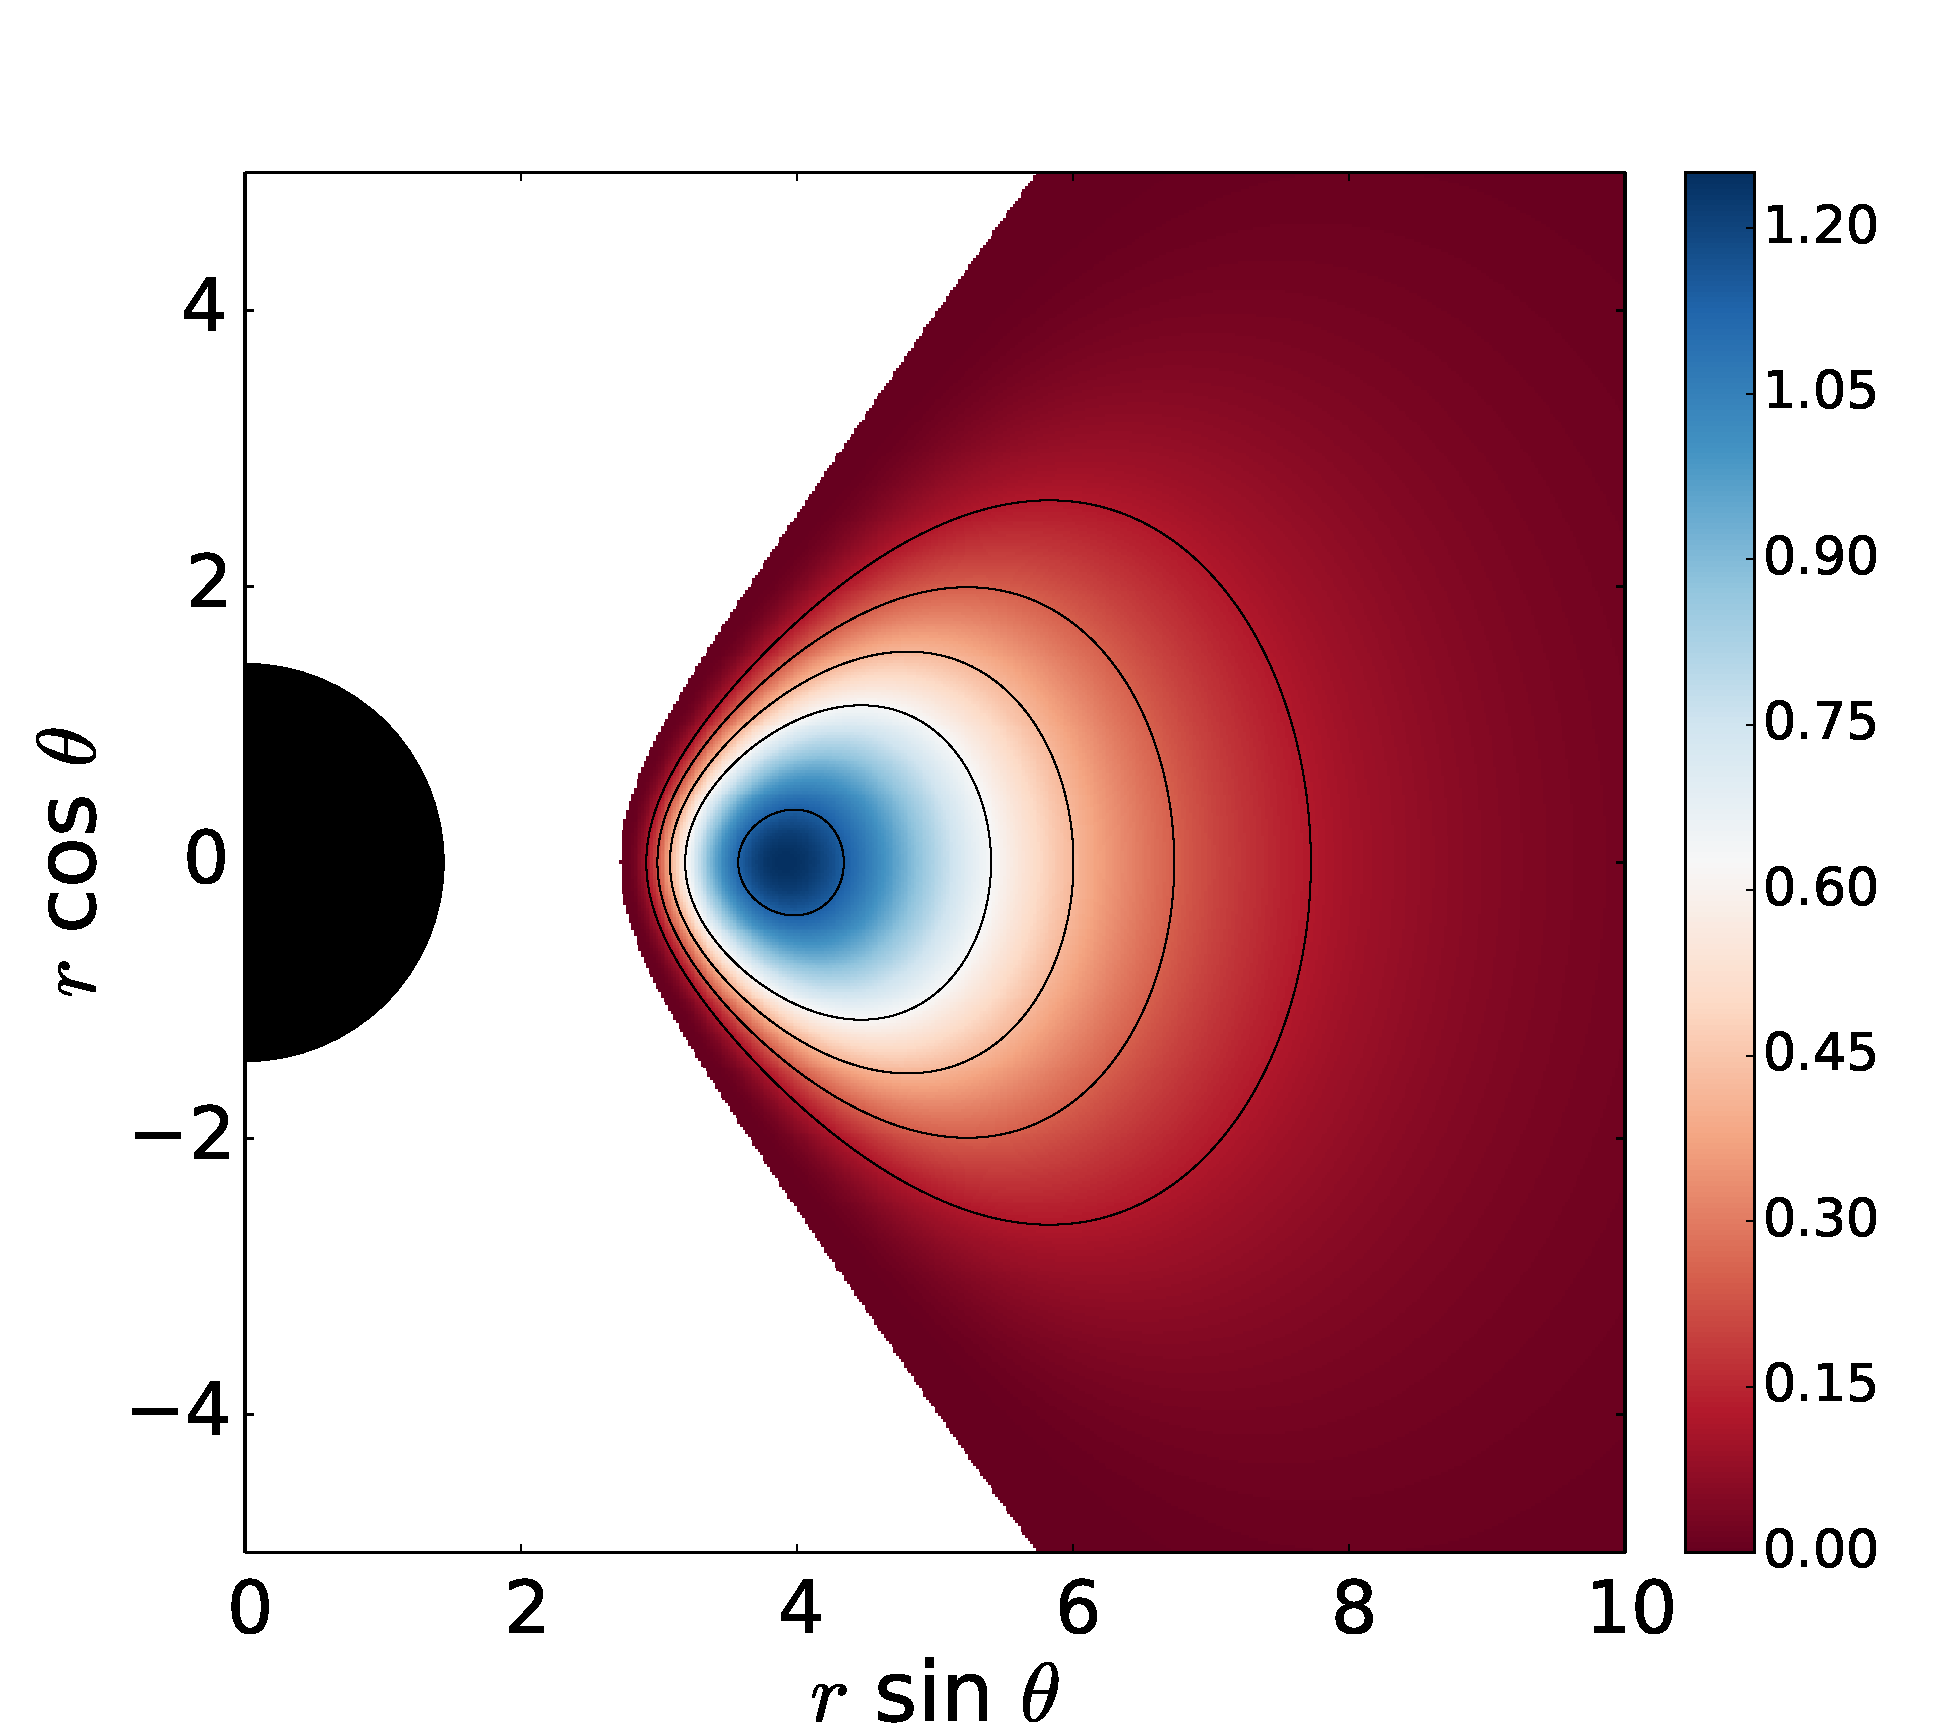
\includegraphics[scale=0.16]{figures/fig1a.pdf}
\hspace{-0.3cm}
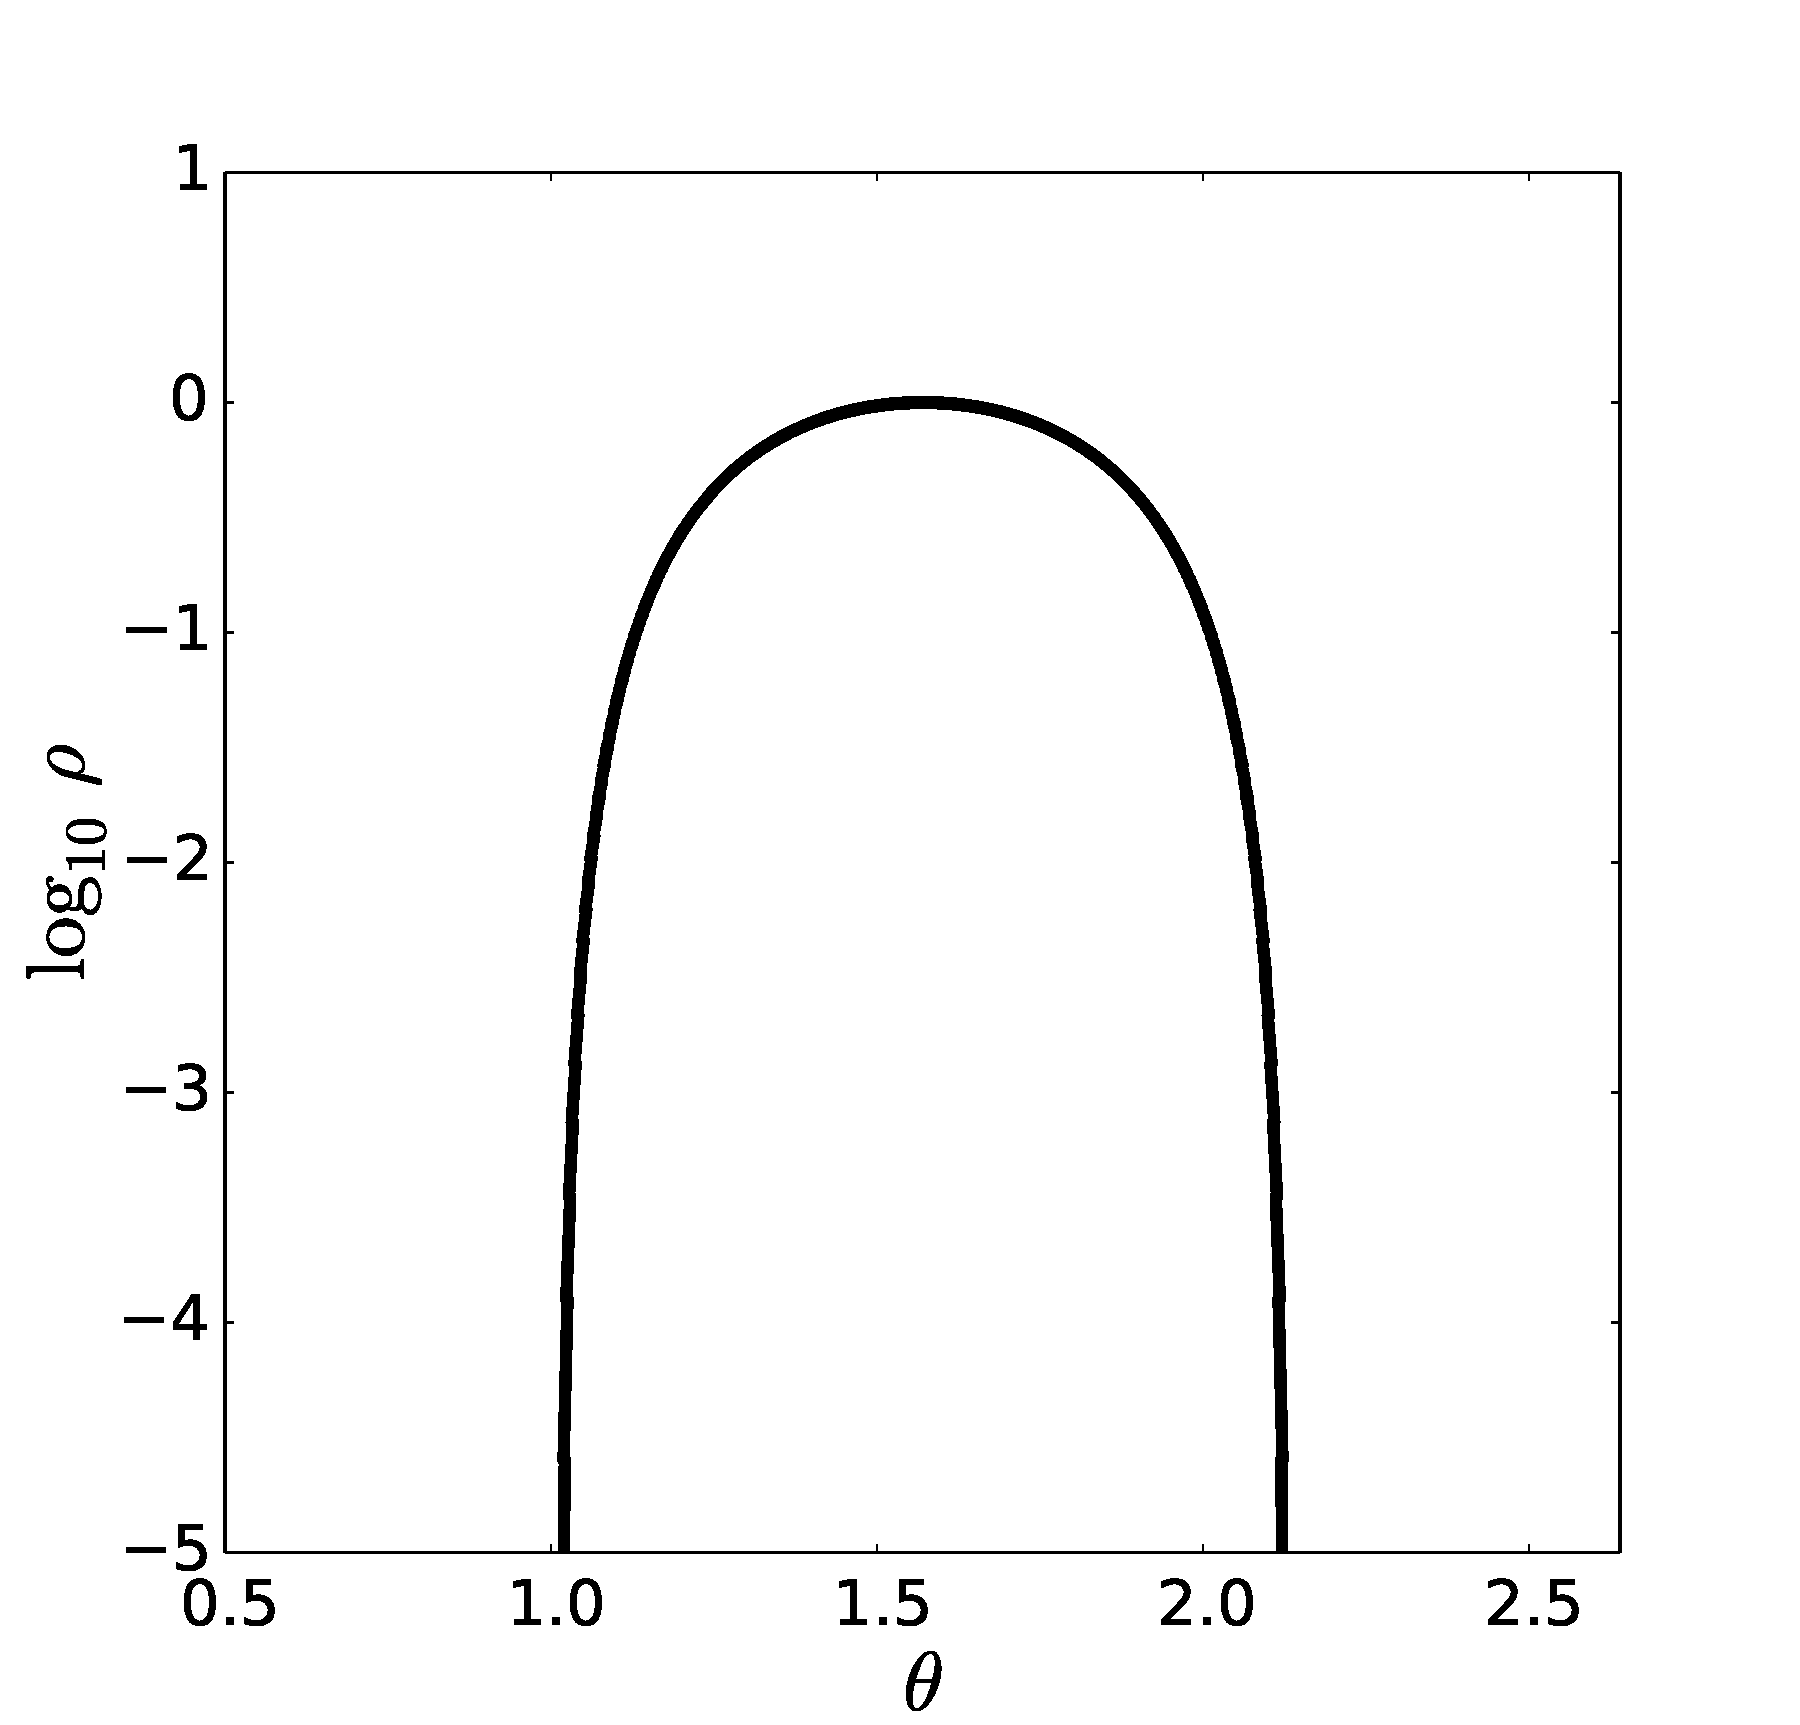
\includegraphics[scale=0.16]{figures/fig1b.pdf}
\hspace{-0.2cm}
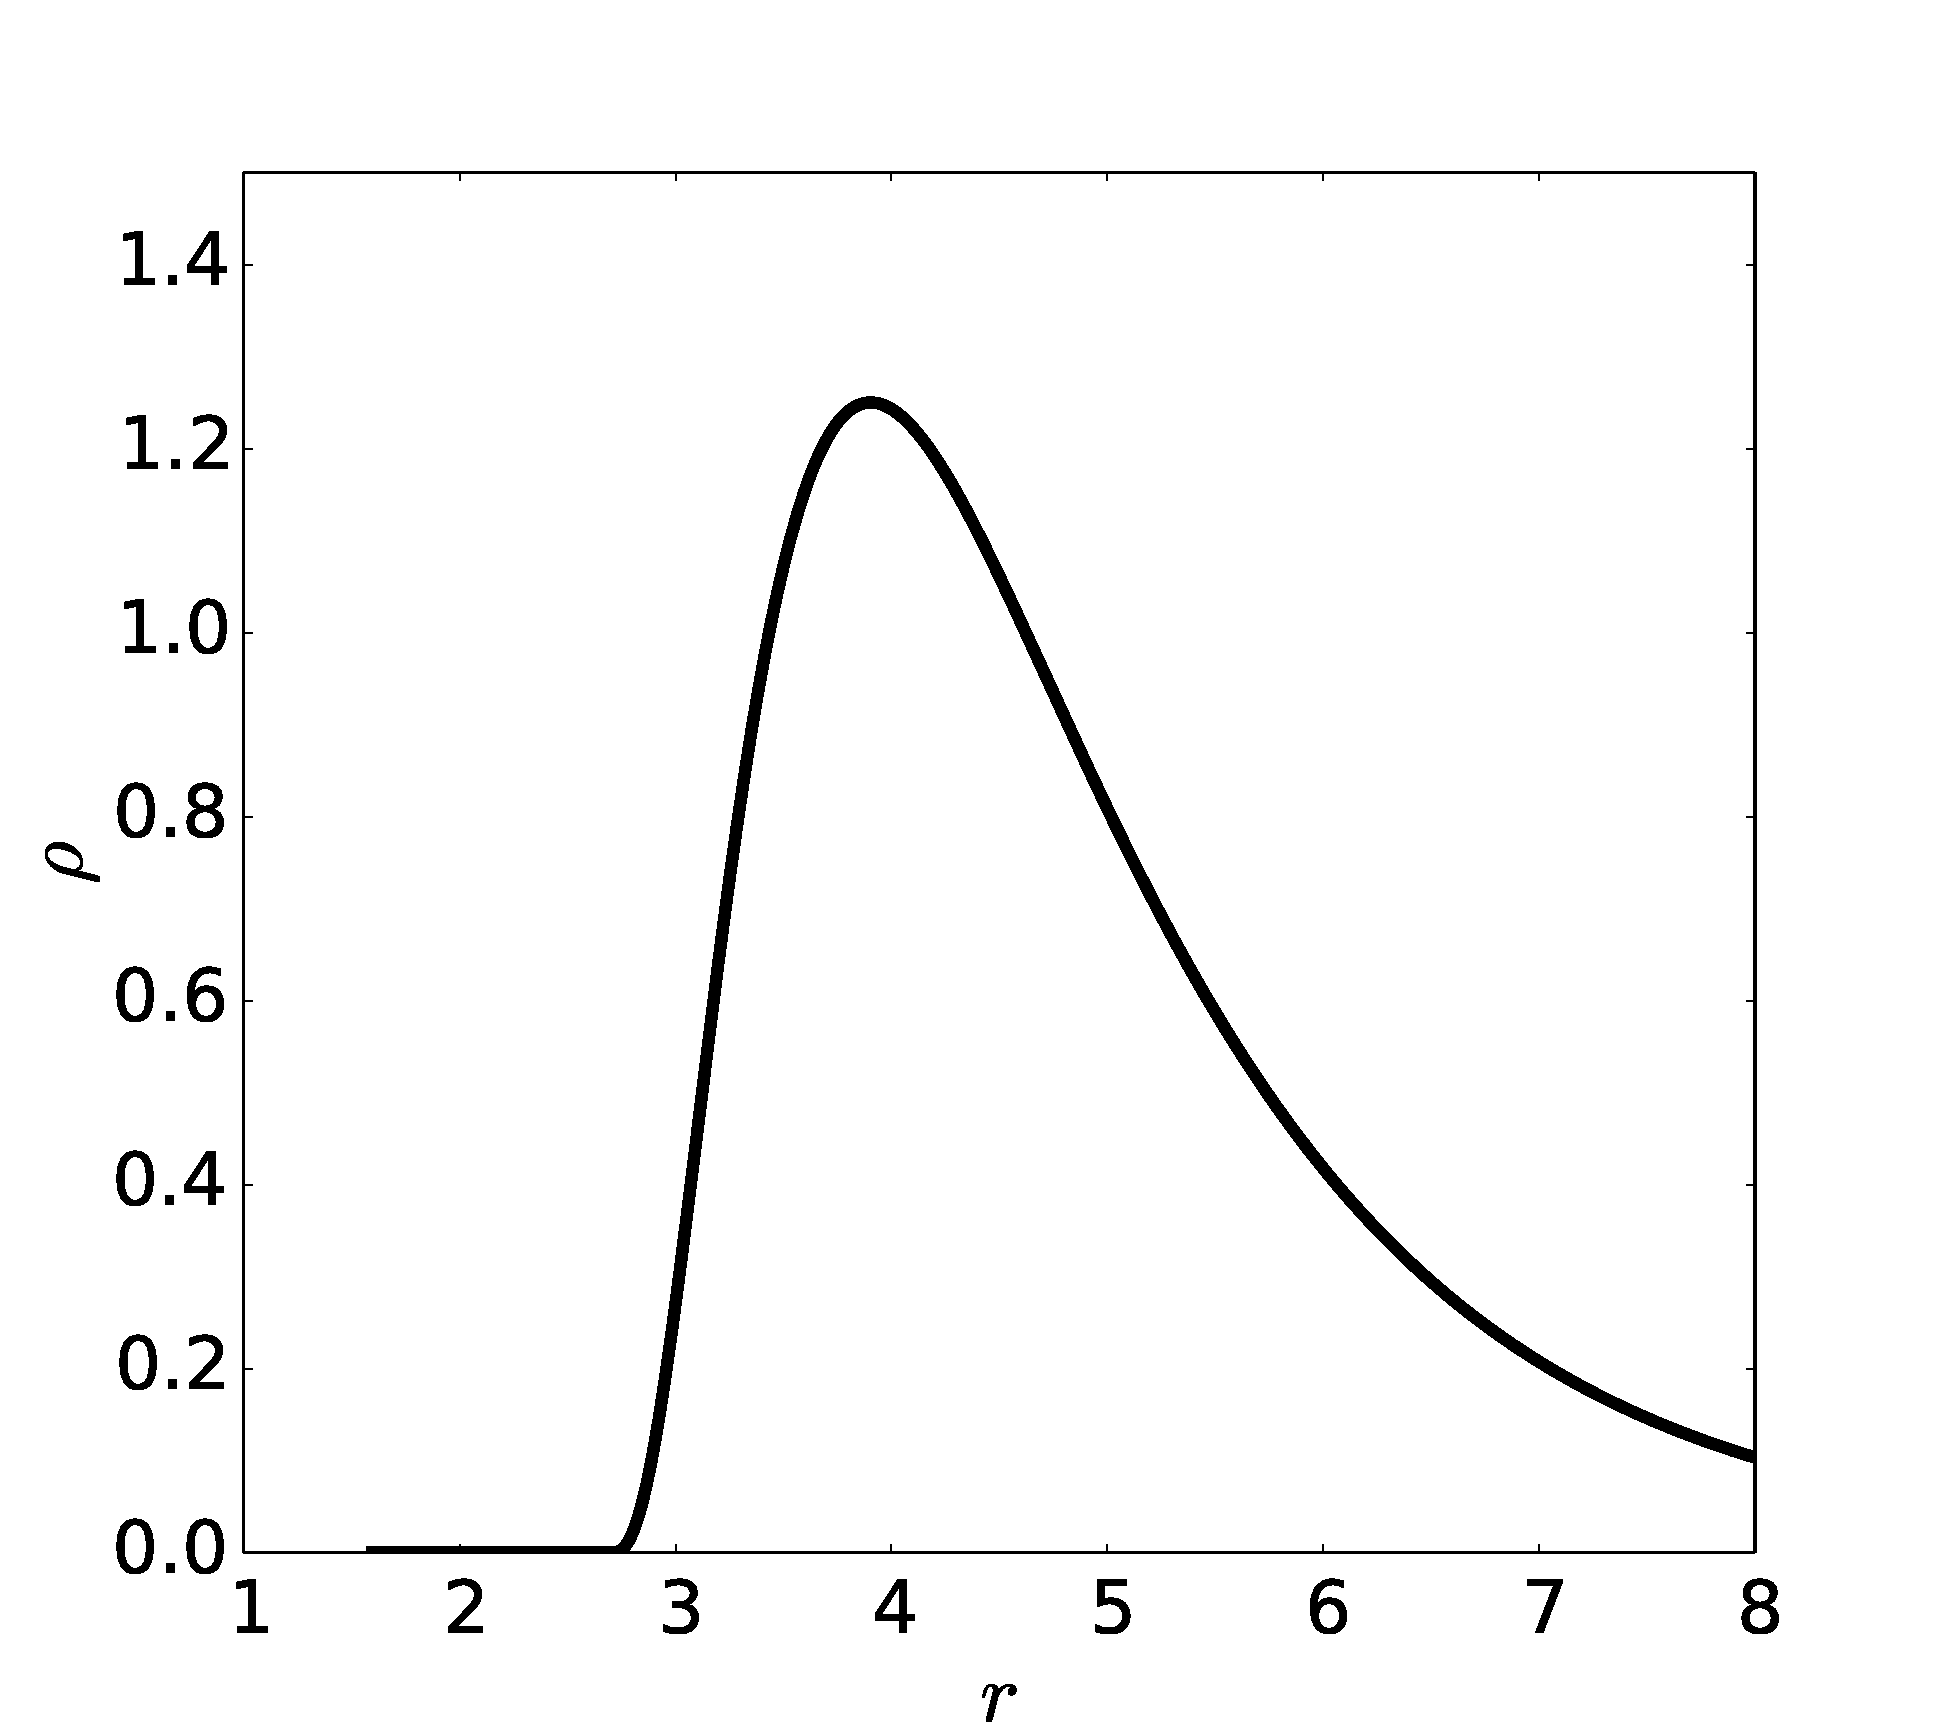
\includegraphics[scale=0.16]{figures/fig1c.pdf}
\caption{Comparison with Komissarov's solution for a constant angular momentum model. The left panel shows the density distribution in logarithm scale for all radii and all angles while the middle and right panels show, respectively, the angular profile of the logarithm of the density at the centre of the disk and the radial profile of the density at the equatorial plane.}
           \label{komissarov}%
 \end{figure*}

Integrating Eq.~\eqref{eq:diff_ver} we obtain
\begin{equation}\label{eq:pre_full_int}
\ln |u_t| - \int^l_0 \frac{\Omega \mathrm{d}l}{1 - \Omega l} + \int^p_0 \frac{\mathrm{d}p}{w} + \int_0^{\tilde{p}_{\mathrm{m}}} \frac{\mathrm{d}\tilde{p}_{\mathrm{m}}}{\tilde{w}} = \mathrm{const}.
\end{equation}
On the surface of the disk, and particularly on its inner edge, the conditions
$p = \tilde{p}_{\mathrm{m}} = 0, \; u_t = u_{t, \mathrm{in}}, \; l = l_{\mathrm{in}}$
are satisfied and, therefore, the integration constant is simply given by
\begin{equation}
\mathrm{const.} = \ln |u_t| - \int^l_{l_\mathrm{in}} \frac{\Omega \mathrm{d}l}{1 - \Omega l}\,.
\end{equation}
We can also introduce the total (gravitational plus centrifugal) potential $W$~\citep{Abramowicz:1978} and write the integral form of the equation of motion as
\begin{equation}\label{eq:potential}
W - W_{\mathrm{in}} = \ln|u_t| - \ln|u_{t,\mathrm{in}}| - \int^{l}_{l_{\mathrm{in}}} \frac{\Omega \mathrm{d}l}{1 - \Omega l},
\end{equation}
where $W_{\mathrm{in}}$ is the potential at the inner edge of the disk (in the equatorial plane). With this definition, we can write Eq.~\eqref{eq:pre_full_int} as
\begin{equation}\label{eq:full_int}
W - W_{\mathrm{in}} = \int^p_0 \frac{\mathrm{d}p}{w} + \int_0^{\tilde{p}_{\mathrm{m}}} \frac{\mathrm{d}\tilde{p}_{\mathrm{m}}}{\tilde{w}},
\end{equation}
which for a barotropic equation of state can be easily integrated to give
\begin{equation}\label{eq:pre_enthalpy_eq}
W - W_{\rm{in}} + \frac{\kappa}{\kappa - 1}\frac{p}{w} + \frac{\lambda
}{\lambda
 - 1}\frac{p_{\mathrm{m}}}{w} = 0\,.
\end{equation}
Replacing $p$ and $p_{\mathrm{m}}$ by equations \eqref{eq:eos_fluid} and \eqref{eq:eos_mag}, the previous equation reduces to
\begin{equation}\label{eq:enthalpy_eq}
W - W_{\rm{in}} + \frac{\kappa}{\kappa - 1} K w^{\kappa - 1} + \frac{\lambda
}{\lambda
 - 1}K_{\mathrm{m}}(\mathcal{L} w)^{\lambda
 - 1} = 0,
\end{equation}
which relates the distribution of the potential with the distribution of enthalpy.

%%%%%%%%%%%%
\section{Methodology}
\label{methodology}
%%%%%%%%%%%%




%\subsection{Building the disk}

To construct the magnetized disks we follow the approach described in \citet{Qian:2009}. First, we find the radial location of the cusp and of the centre of the disk in the equatorial plane, $r_{\mathrm{cusp}}$ and $r_{\mathrm{c}}$, defined as the solutions to the equation $l(r) - l_{\mathrm{K}} = 0$.
Next, we compute the partial derivatives of the potential, Eq.~\eqref{eq:potential}
\begin{equation}\label{eq:radial_der_pot}
\partial_r W = \partial_r \ln|u_t| - \frac{\Omega \partial_rl}{1 - \Omega l}\,,
\end{equation}
and
\begin{equation}\label{eq:polar_der_pot}
\partial_{\theta} W = \partial_{\theta} \ln|u_t| - \frac{\Omega \partial_{\theta}l}{1 - \Omega l}\,.
\end{equation}
Then, we integrate the radial partial derivative of the potential along the segment $[r_{\mathrm{cusp}}, r_{\mathrm{c}}]$ (assuming $W_{\mathrm{cusp}} = 0$) at the equatorial plane, thus obtaining the equatorial distribution of the potential between $r_{\mathrm{cusp}}$ and $r_{\mathrm{c}}$
\begin{equation}\label{eq:equatorial_pot}
W_{\mathrm{eq}}(r) = \int^{r}_{r_{\mathrm{cusp}}}\left(\partial_r \ln|u_t| - \frac{\Omega \partial_rl}{1 - \Omega l}\right).
\end{equation}
Following \citet{Qian:2009} we can divide equations \eqref{eq:radial_der_pot} and \eqref{eq:polar_der_pot} to obtain
\begin{equation}\label{eq:F}
F(r, \theta) = -\frac{\partial_r W}{\partial_{\theta} W} = \frac{\mathrm{d}\theta}{\mathrm{d}r}\,,
\end{equation}
which is an ordinary differential equation that can be integrated to obtain the location of the equipotential surfaces.

Next, we choose all the initial values for the integration of the equation \eqref{eq:F} to be between $r_{\mathrm{cusp}}$ and $r_{\mathrm{c}}$ ($\theta = \pi / 2$). Since we are only interested in the surfaces inside the Roche lobe, our choice of initial values provides us a mapping of the equipotential surfaces of the torus. Given that we have already obtained both the equipotential surfaces which cross the segment $[r_{\mathrm{cusp}}, r_{\mathrm{c}}]$ and the potential distribution there, we found the potential distribution for the torus.
Once we have the potential distribution, we can find the gas pressure at the center, from equation \eqref{eq:enthalpy_eq}
\begin{equation}
p_{\mathrm{c}} = w_{\mathrm{c}}(W_{\mathrm{in}} - W_{\mathrm{c}})\left(\frac{\kappa}{\kappa - 1} + \frac{\lambda
}{\lambda
 - 1}\frac{1}{\beta_{\mathrm{m}_{\mathrm{c}}}}\right)^{-1},
\end{equation}
where $w_{\mathrm{c}}$ is the enthalpy at the disk center and
\begin{equation}
\label{eq:beta_eq}
\beta_{\mathrm{m}} = p/p_{\mathrm{m}},
\end{equation}
is the magnetization parameter (being $\beta_{\mathrm{m}_{\mathrm{c}}}$ the magnetization parameter at the disk center). By this definition, we can find the magnetic pressure at the disk center,
\begin{equation}
p_{\mathrm{m_{\mathrm{c}}}} = p_{\mathrm{c}}/\beta_{\mathrm{m}_{\mathrm{c}}}
\end{equation}
With the pressures at the center, we can also find the constants $K$ and $K_{\mathrm{m}}$ using the equations \eqref{eq:eos_fluid} and \eqref{eq:eos_mag}. And, for a given inner radius of the disk $r_{\mathrm{in}}$ we can find the potential $W_{\mathrm{in}}$. We now have all the elements required to find the enthalpy distribution (equation \eqref{eq:enthalpy_eq}), the pressure and magnetic pressure distribution (equations \eqref{eq:eos_fluid} and \eqref{eq:eos_mag}), and the density (equation \eqref{eq:density_eq}).

 
%\subsection{Numerical code}

For the integration of equation \eqref{eq:equatorial_pot} we use the composite Simpson's rule, it is important to use a very small step of integration, because the slope is very steep. In this work, we use a step $h = 10^{-6}$ . A bigger step gives an unacceptable lack of accuracy, we tested that fact by comparison with the analytic, constant angular momentum case.

To integrate the ordinary differential equation \eqref{eq:F} we use a fourth-order Runge-Kutta method. Here is also important to choose a suitable step of integration, specially at the outer end of the disk, this is because the equation \eqref{eq:F} diverges of the equatorial plane (the equipotential surfaces crosses the equatorial plane perpendicularly).

%\subsection{Parameter space}

As in \citet{Komissarov:2006}, in this paper we have chosen the exponents $\kappa = \lambda
 = 4/3$ and the enthalpy at the disk center $w_{\mathrm{c}} = 1$. That leaves us the magnetization parameter $\beta_{\mathrm{m}_{\mathrm{c}}}
$, the parameters of the angular momentum distribution $\beta$ and $\gamma$, the black hole spin parameter $a$ and the inner radius of the disk $r_{\mathrm{in}}$. This allows us to control the size, shape, thickness and magnetization of the disk.

% \begin{table}
% \caption{List of models. Form left to right the columns report: the black hole spin $a$, the parameters of the angular momentum distribution $\beta$ and $\gamma$, the magnetization parameter $\beta_{\mathrm{m}_{\mathrm{c}}}
% $ at the disk center, the corresponding radii of the maximum thermal pressure and magnetic pressure, $r_{{\rm{max}}}$ and $r_{{\mathrm{m, max}}}$, the gravitational potential diference between the center and the inner radius, $\Delta W\equiv W_{\rm c}-W_{\rm in}$, and the inner and outer radii of the disks, $r_{\mathrm{in}}$ and  $r_{\mathrm{out}}$.}             
% \label{table:1}      
% \centering          
% \begin{tabular}{c c c c c c  c c c c}
% \hline\hline       
%  & $a$ & $\beta$ & $\gamma$ & $\beta_{\mathrm{m}_{\mathrm{c}}}
% $  & $r_{\rm{max}}$ &  $r_{\mathrm{m, max}}$ & $\Delta W$ & $r_{\mathrm{in}}$ & $r_{\mathrm{out}}$ \\ 
% \hline           
% A1 & $0.5$ & $0.0$ & $0.0$ & $10^{-3}$ &  $5.11$  & $5.51$ & $-6.35 \times 10^{-2}$ & $2.91$ & -- \\ 
% A2 &           & $0.5$ & $0.5$ &  & $5.55$ &  $5.80$  & $-2.27 \times 10^{-2}$ & $3.20$ & $11.77$\\ 
% A3  &          & $0.9$ & $0.9$ &  & $5.95$ &  $6.15$  & $-2.96 \times 10^{-3}$ & $3.70$ &  $9.583$\\ 
% A4  &          & $0.0$ & $0.9$ &  & $5.21$ &  $5.51$  & $-6.35 \times 10^{-2}$ & $2.91$ & $9.680$\\ 
% A5   &         & $0.9$ & $0.0$ &  & $5.90$ &  $6.10$  & $-2.95 \times 10^{-3}$ & $3.70$ & --\\ 
%  \hline 
% B1 & $0.9$ & $0.0$ & $0.0$ & $10^{-3}$ & $2.53$ &  $2.73$  & $-0.129$ & $1.73$ & -- \\ 
% B2 &           & $0.5$ & $0.5$ &  & $2.81$ &  $2.91$  & $-4.32 \times 10^{-2}$ & $1.86$ & $5.35$\\ 
% B3  &          & $0.9$ & $0.9$ &  & $3.03$ &  $3.13$  & $-5.39 \times 10^{-3}$ & $2.08$ & $4.52$\\ 
% B4  &          & $0.0$ & $0.9$ &  & $2.65$ &  $2.80$  & $-0.129$ & $1.732$ & $4.54$\\ 
% B5   &         & $0.9$ & $0.0$ &  & $3.03$ &  $3.13$  & $-5.39 \times 10^{-3}$ & $2.08$ & -- \\  
%  \hline 
% C1 & $0.99$ & $0.0$ & $0.0$ & $10^{-3}$ & $1.46$ & $1.51$ & $-0.246$ & $1.21$ & -- \\ 
% C2 &             & $0.5$ & $0.5$ &  & $1.56$ &  $1.61$  & $-7.34 \times 10^{-2}$ & $1.26$ & $2.50$\\ 
% C3  &            & $0.9$ & $0.9$ &  & $1.70$ &  $1.75$  & $-8.53 \times 10^{-3}$ & $1.35$ & $2.25$\\ 
% C4  &            & $0.0$ & $0.9$ &  & $1.50$ &  $1.57$  & $-0.246$ & $1.21$ & $2.26$\\ 
% C5   &           & $0.9$ & $0.0$ &  & $1.72$ &  $1.77$  & $-8.53 \times 10^{-3}$ & $1.35$ & --\\ 
% \hline      
% \end{tabular}
% \end{table}

\begin{table}
\caption{List of models for $\beta_{\mathrm{m}_{\mathrm{c}}} = 10^{3}
$. Form left to right the columns report: the model name (with A, B and C standing for black hole spin $a = 0.5$, $0.9$ and $0.99$ respectively), the parameters of the angular momentum distribution $\beta$ and $\gamma$, , the corresponding radii of the maximum thermal pressure and magnetic pressure, $r_{{\rm{max}}}$ and $r_{{\mathrm{m, max}}}$, the gravitational potential diference between the center and the inner radius, $\Delta W\equiv W_{\rm c}-W_{\rm in}$, and the inner and outer radii of the disks, $r_{\mathrm{in}}$ and $r_{\mathrm{out}}$.}             
\label{table:1}      
\centering          
\begin{tabular}{c c c c  c c c c}
\hline\hline       
 & $\beta$ & $\gamma$ & $r_{\rm{max}}$ &  $r_{\mathrm{m, max}}$ & $\Delta W (\times 10^{-2})$ & $r_{\mathrm{in}}$ & $r_{\mathrm{out}}$ \\ 
\hline           
A1 & $0.0$ & $0.0$ & $7.15$ &  $8.14$  & $-6.35$ & $2.91$ & -- \\ 
A2 & $0.5$ & $0.5$ & $7.15$ &  $7.65$  & $-2.27$ & $3.20$ & $11.8$\\ 
A3 & $0.9$ & $0.9$ & $7.15$ &  $7.45$  & $-0.30$ & $3.70$ &  $9.58$\\ 
A4 & $0.0$ & $0.9$ & $7.15$ &  $8.32$  & $-6.35$ & $2.91$ & $9.68$\\ 
A5 & $0.9$ & $0.0$ & $7.15$ &  $7.28$  & $-0.30$ & $3.70$ & --\\ 
 \hline 
B1 & $0.0$ & $0.0$ & $3.59$ &  $3.98$  & $-12.9$ & $1.73$ & -- \\ 
B2 & $0.5$ & $0.5$ & $3.59$ &  $3.83$  & $-4.32$ & $1.86$ & $5.35$\\ 
B3 & $0.9$ & $0.9$ & $3.59$ &  $3.73$  & $-0.54$ & $2.08$ & $4.52$\\ 
B4 & $0.0$ & $0.9$ & $3.59$ &  $3.85$  & $-12.9$ & $1.73$ & $4.54$\\ 
B5 & $0.9$ & $0.0$ & $3.59$ &  $3.81$  & $-0.54$ & $2.08$ & -- \\  
 \hline 
C1 & $0.0$ & $0.0$ & $1.98$ &  $2.28$  & $-24.6$ & $1.21$ & -- \\ 
C2 & $0.5$ & $0.5$ & $1.98$ &  $2.09$  & $-7.34$ & $1.26$ & $2.50$\\ 
C3 & $0.9$ & $0.9$ & $1.98$ &  $2.04$  & $-0.85$ & $1.35$ & $2.25$\\ 
C4 & $0.0$ & $0.9$ & $1.98$ &  $2.10$  & $-24.6$ & $1.21$ & $2.26$\\ 
C5 & $0.9$ & $0.0$ & $1.98$ &  $2.08$  & $-0.85$ & $1.35$ & --\\ 
\hline      
\end{tabular}
\end{table}

\begin{table}
\caption{List of models for $\beta_{\mathrm{m}_{\mathrm{c}}} = 1
$. Form left to right the columns report: the model name (with A, B and C standing for black hole spin $a = 0.5$, $0.9$ and $0.99$ respectively), the parameters of the angular momentum distribution $\beta$ and $\gamma$, , the corresponding radii of the maximum thermal pressure and magnetic pressure, $r_{{\rm{max}}}$ and $r_{{\mathrm{m, max}}}$, the gravitational potential diference between the center and the inner radius, $\Delta W\equiv W_{\rm c}-W_{\rm in}$, and the inner and outer radii of the disks, $r_{\mathrm{in}}$ and $r_{\mathrm{out}}$.}             
\label{table:3}      
\centering          
\begin{tabular}{c c c c  c c c c}
\hline\hline       
 & $\beta$ & $\gamma$ & $r_{\rm{max}}$ &  $r_{\mathrm{m, max}}$ & $\Delta W (\times 10^{-2})$ & $r_{\mathrm{in}}$ & $r_{\mathrm{out}}$ \\ 
\hline           
A1 & $0.0$ & $0.0$ & $6.00$ &  $6.49$  & $-6.35$ & $2.91$ & -- \\ 
A2 & $0.5$ & $0.5$ & $6.25$ &  $6.66$  & $-2.27$ & $3.20$ & $11.8$\\ 
A3 & $0.9$ & $0.9$ & $6.50$ &  $6.80$  & $-0.30$ & $3.70$ &  $9.58$\\ 
A4 & $0.0$ & $0.9$ & $6.00$ &  $6.49$  & $-6.35$ & $2.91$ & $9.68$\\ 
A5 & $0.9$ & $0.0$ & $6.50$ &  $6.80$  & $-0.30$ & $3.70$ & --\\ 
 \hline 
B1 & $0.0$ & $0.0$ & $3.02$ &  $3.26$  & $-12.9$ & $1.73$ & -- \\ 
B2 & $0.5$ & $0.5$ & $3.16$ &  $3.35$  & $-4.32$ & $1.86$ & $5.35$\\
B3 & $0.9$ & $0.9$ & $3.29$ &  $3.43$  & $-0.54$ & $2.08$ & $4.52$\\ 
B4 & $0.0$ & $0.9$ & $3.02$ &  $3.26$  & $-12.9$ & $1.73$ & $4.54$\\  
B5 & $0.9$ & $0.0$ & $3.29$ &  $3.43$  & $-0.54$ & $2.08$ & -- \\ 
 \hline 
C1 & $0.0$ & $0.0$ & $1.68$ &  $1.80$  & $-0.246$ & $1.21$ & -- \\ 
C2 & $0.5$ & $0.5$ & $1.77$ &  $1.86$  & $-7.34$ & $1.26$ & $2.50$\\  
C3 & $0.9$ & $0.9$ & $1.84$ &  $1.91$  & $-0.85$ & $1.35$ & $2.25$\\ 
C4 & $0.0$ & $0.9$ & $1.68$ &  $1.80$  & $-24.6$ & $1.21$ & $2.26$\\ 
C5 & $0.9$ & $0.0$ & $1.84$ &  $1.91$  & $-0.85$ & $1.35$ & --\\ 
\hline      
\end{tabular}
\end{table}

\begin{table}
\caption{List of models for $\beta_{\mathrm{m}_{\mathrm{c}}} = 10^{-3}
$. Form left to right the columns report: the model name (with A, B and C standing for black hole spin $a = 0.5$, $0.9$ and $0.99$ respectively), the parameters of the angular momentum distribution $\beta$ and $\gamma$, , the corresponding radii of the maximum thermal pressure and magnetic pressure, $r_{{\rm{max}}}$ and $r_{{\mathrm{m, max}}}$, the gravitational potential diference between the center and the inner radius, $\Delta W\equiv W_{\rm c}-W_{\rm in}$, and the inner and outer radii of the disks, $r_{\mathrm{in}}$ and $r_{\mathrm{out}}$.}             
\label{table:3}      
\centering          
\begin{tabular}{c c c c  c c c c}
\hline\hline       
 & $\beta$ & $\gamma$ & $r_{\rm{max}}$ &  $r_{\mathrm{m, max}}$ & $\Delta W (\times 10^{-2})$ & $r_{\mathrm{in}}$ & $r_{\mathrm{out}}$ \\ 
\hline           
A1 & $0.0$ & $0.0$ & $5.11$ &  $5.51$  & $-6.35$ & $2.91$ & -- \\ 
A2 & $0.5$ & $0.5$ & $5.55$ &  $5.80$  & $-2.27$ & $3.20$ & $11.8$\\ 
A3 & $0.9$ & $0.9$ & $5.95$ &  $6.15$  & $-0.30$ & $3.70$ &  $9.58$\\ 
A4 & $0.0$ & $0.9$ & $5.21$ &  $5.51$  & $-6.35$ & $2.91$ & $9.68$\\  
A5 & $0.9$ & $0.0$ & $5.90$ &  $6.10$  & $-0.30$ & $3.70$ & --\\
 \hline 
B1 & $0.0$ & $0.0$ & $2.53$ &  $2.73$  & $-12.9$ & $1.73$ & -- \\ 
B2 & $0.5$ & $0.5$ & $2.81$ &  $2.91$  & $-4.32$ & $1.86$ & $5.35$\\
B3 & $0.9$ & $0.9$ & $3.03$ &  $3.13$  & $-0.54$ & $2.08$ & $4.52$\\  
B4 & $0.0$ & $0.9$ & $2.65$ &  $2.80$  & $-12.9$ & $1.73$ & $4.54$\\ 
B5 & $0.9$ & $0.0$ & $3.03$ &  $3.13$  & $-0.54$ & $2.08$ & -- \\  
 \hline 
C1 & $0.0$ & $0.0$ & $1.46$ &  $1.51$  & $-24.6$ & $1.21$ & -- \\ 
C2 & $0.5$ & $0.5$ & $1.56$ &  $1.61$  & $-7.34$ & $1.26$ & $2.50$\\ 
C3 & $0.9$ & $0.9$ & $1.70$ &  $1.75$  & $-0.85$ & $1.35$ & $2.25$\\ 
C4 & $0.0$ & $0.9$ & $1.50$ &  $1.57$  & $-24.6$ & $1.21$ & $2.26$\\ 
C5 & $0.9$ & $0.0$ & $1.72$ &  $1.77$  & $-0.85$ & $1.35$ & --\\ 
\hline      
\end{tabular}
\end{table}

%%%%%%%%%
\section{Results}
\label{results}
%%%%%%%%%

\begin{figure*}
\centering
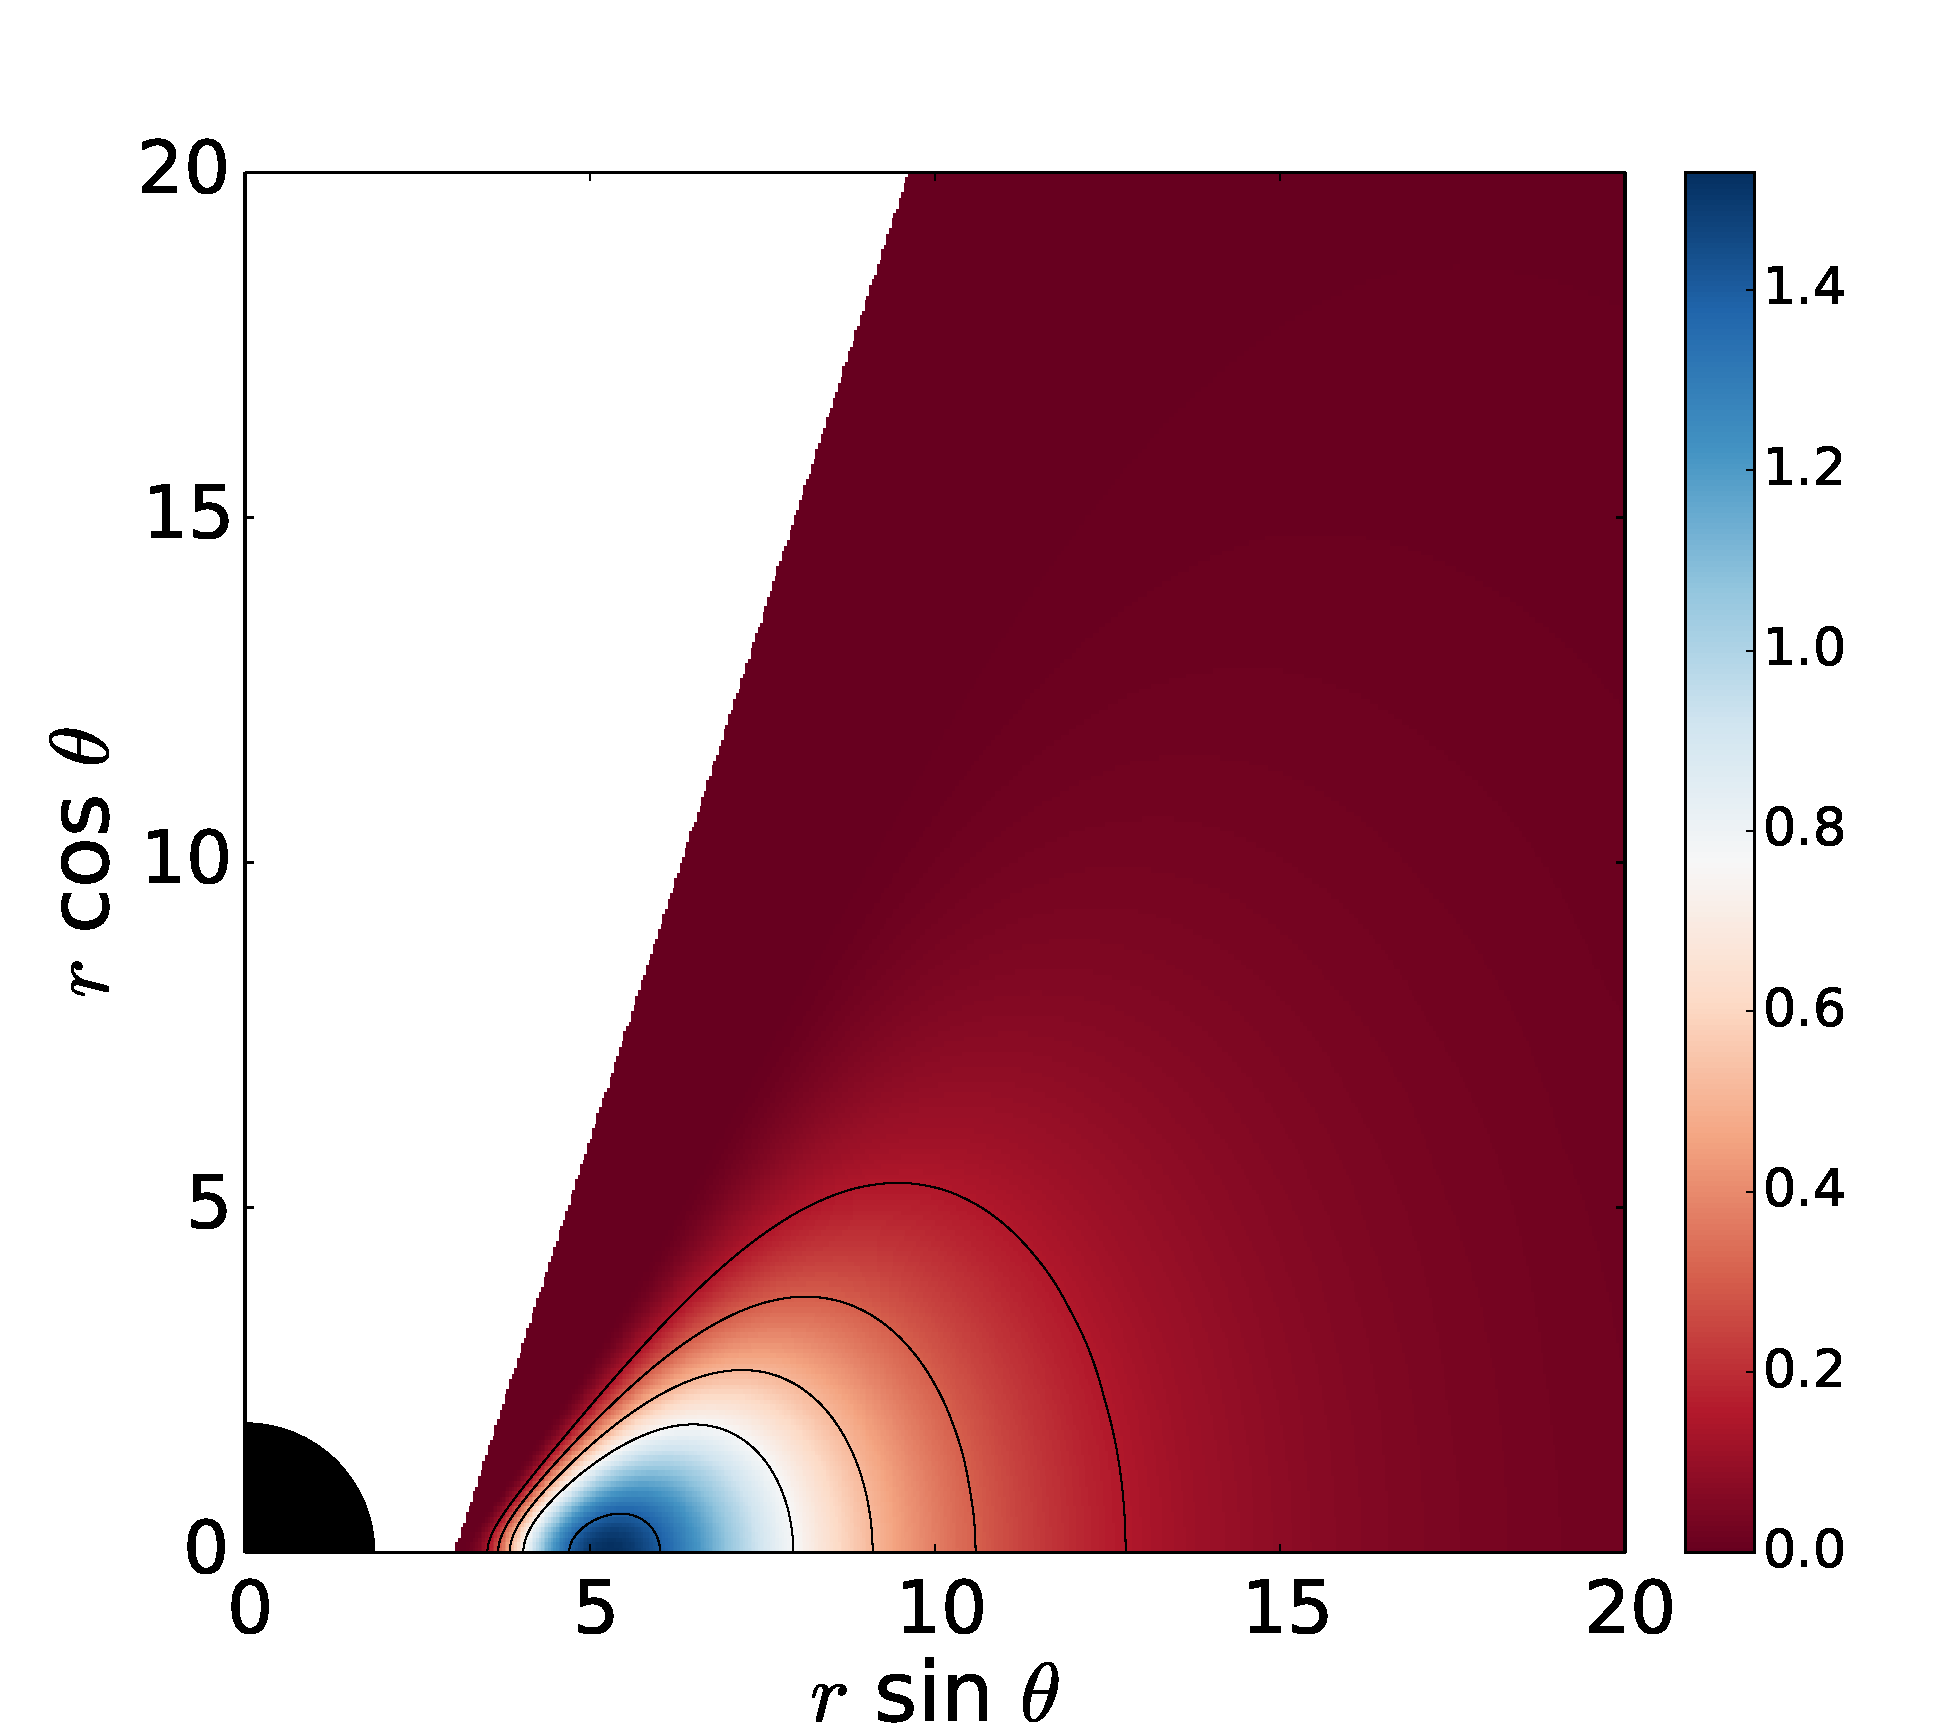
\includegraphics[scale=0.16]{figures/fig2_1_1.pdf}
\hspace{-0.3cm}
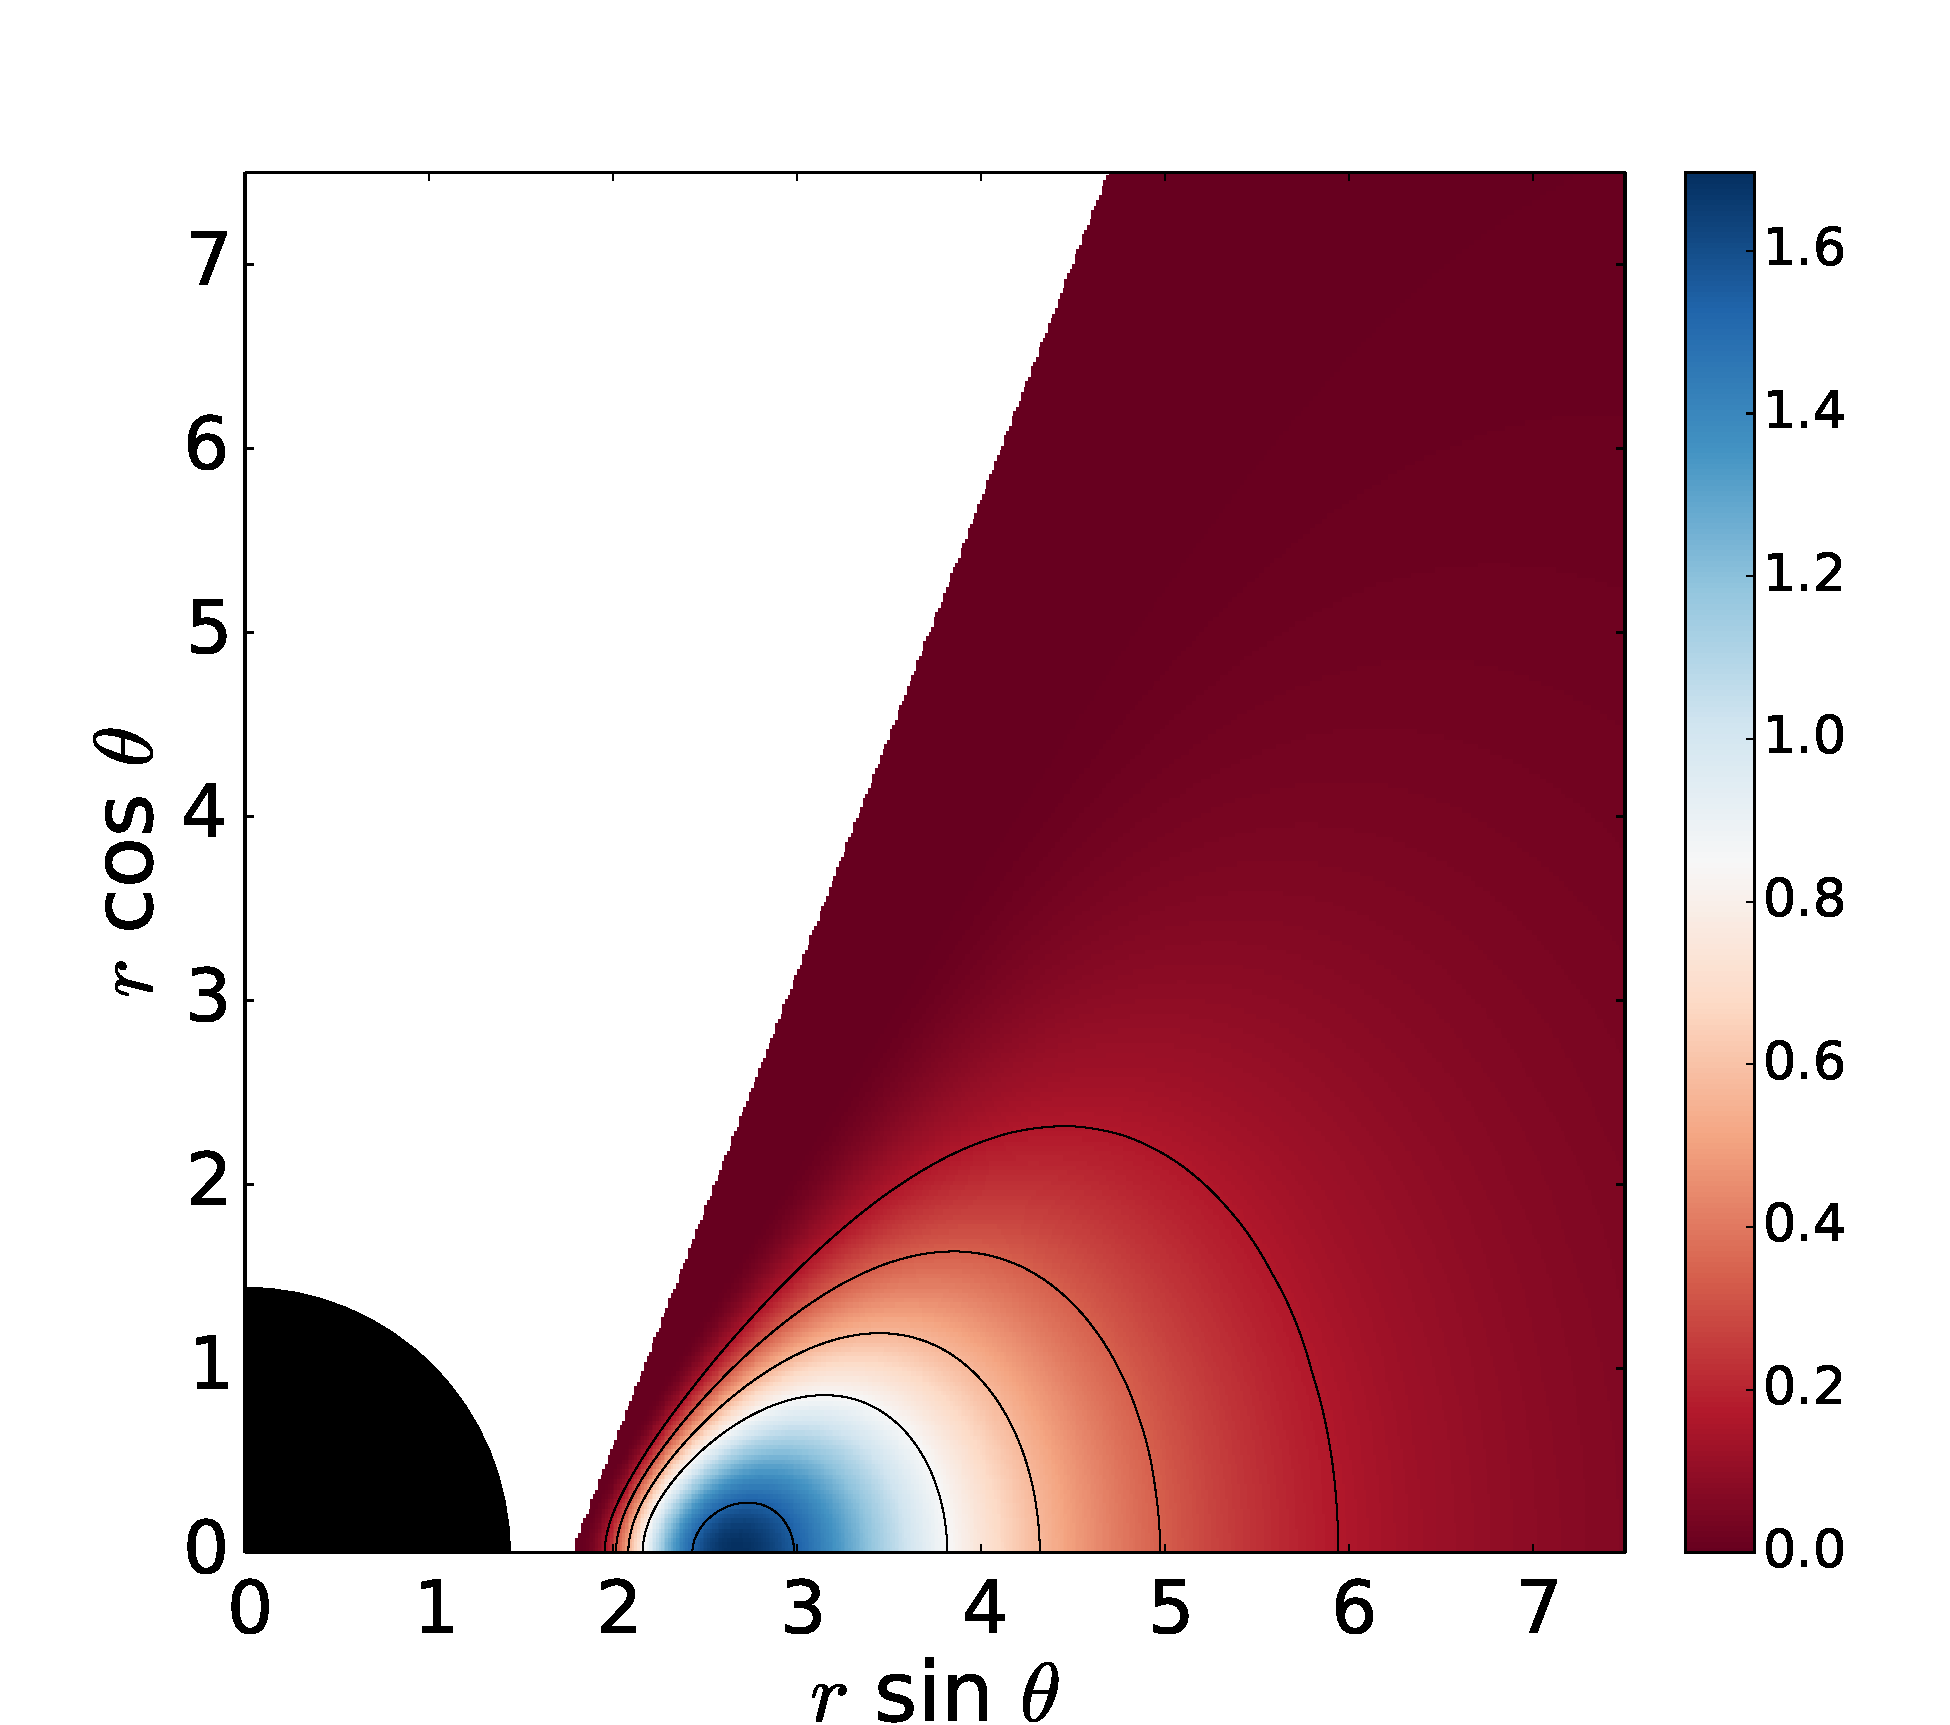
\includegraphics[scale=0.16]{figures/fig2_1_2.pdf}
\hspace{-0.2cm}
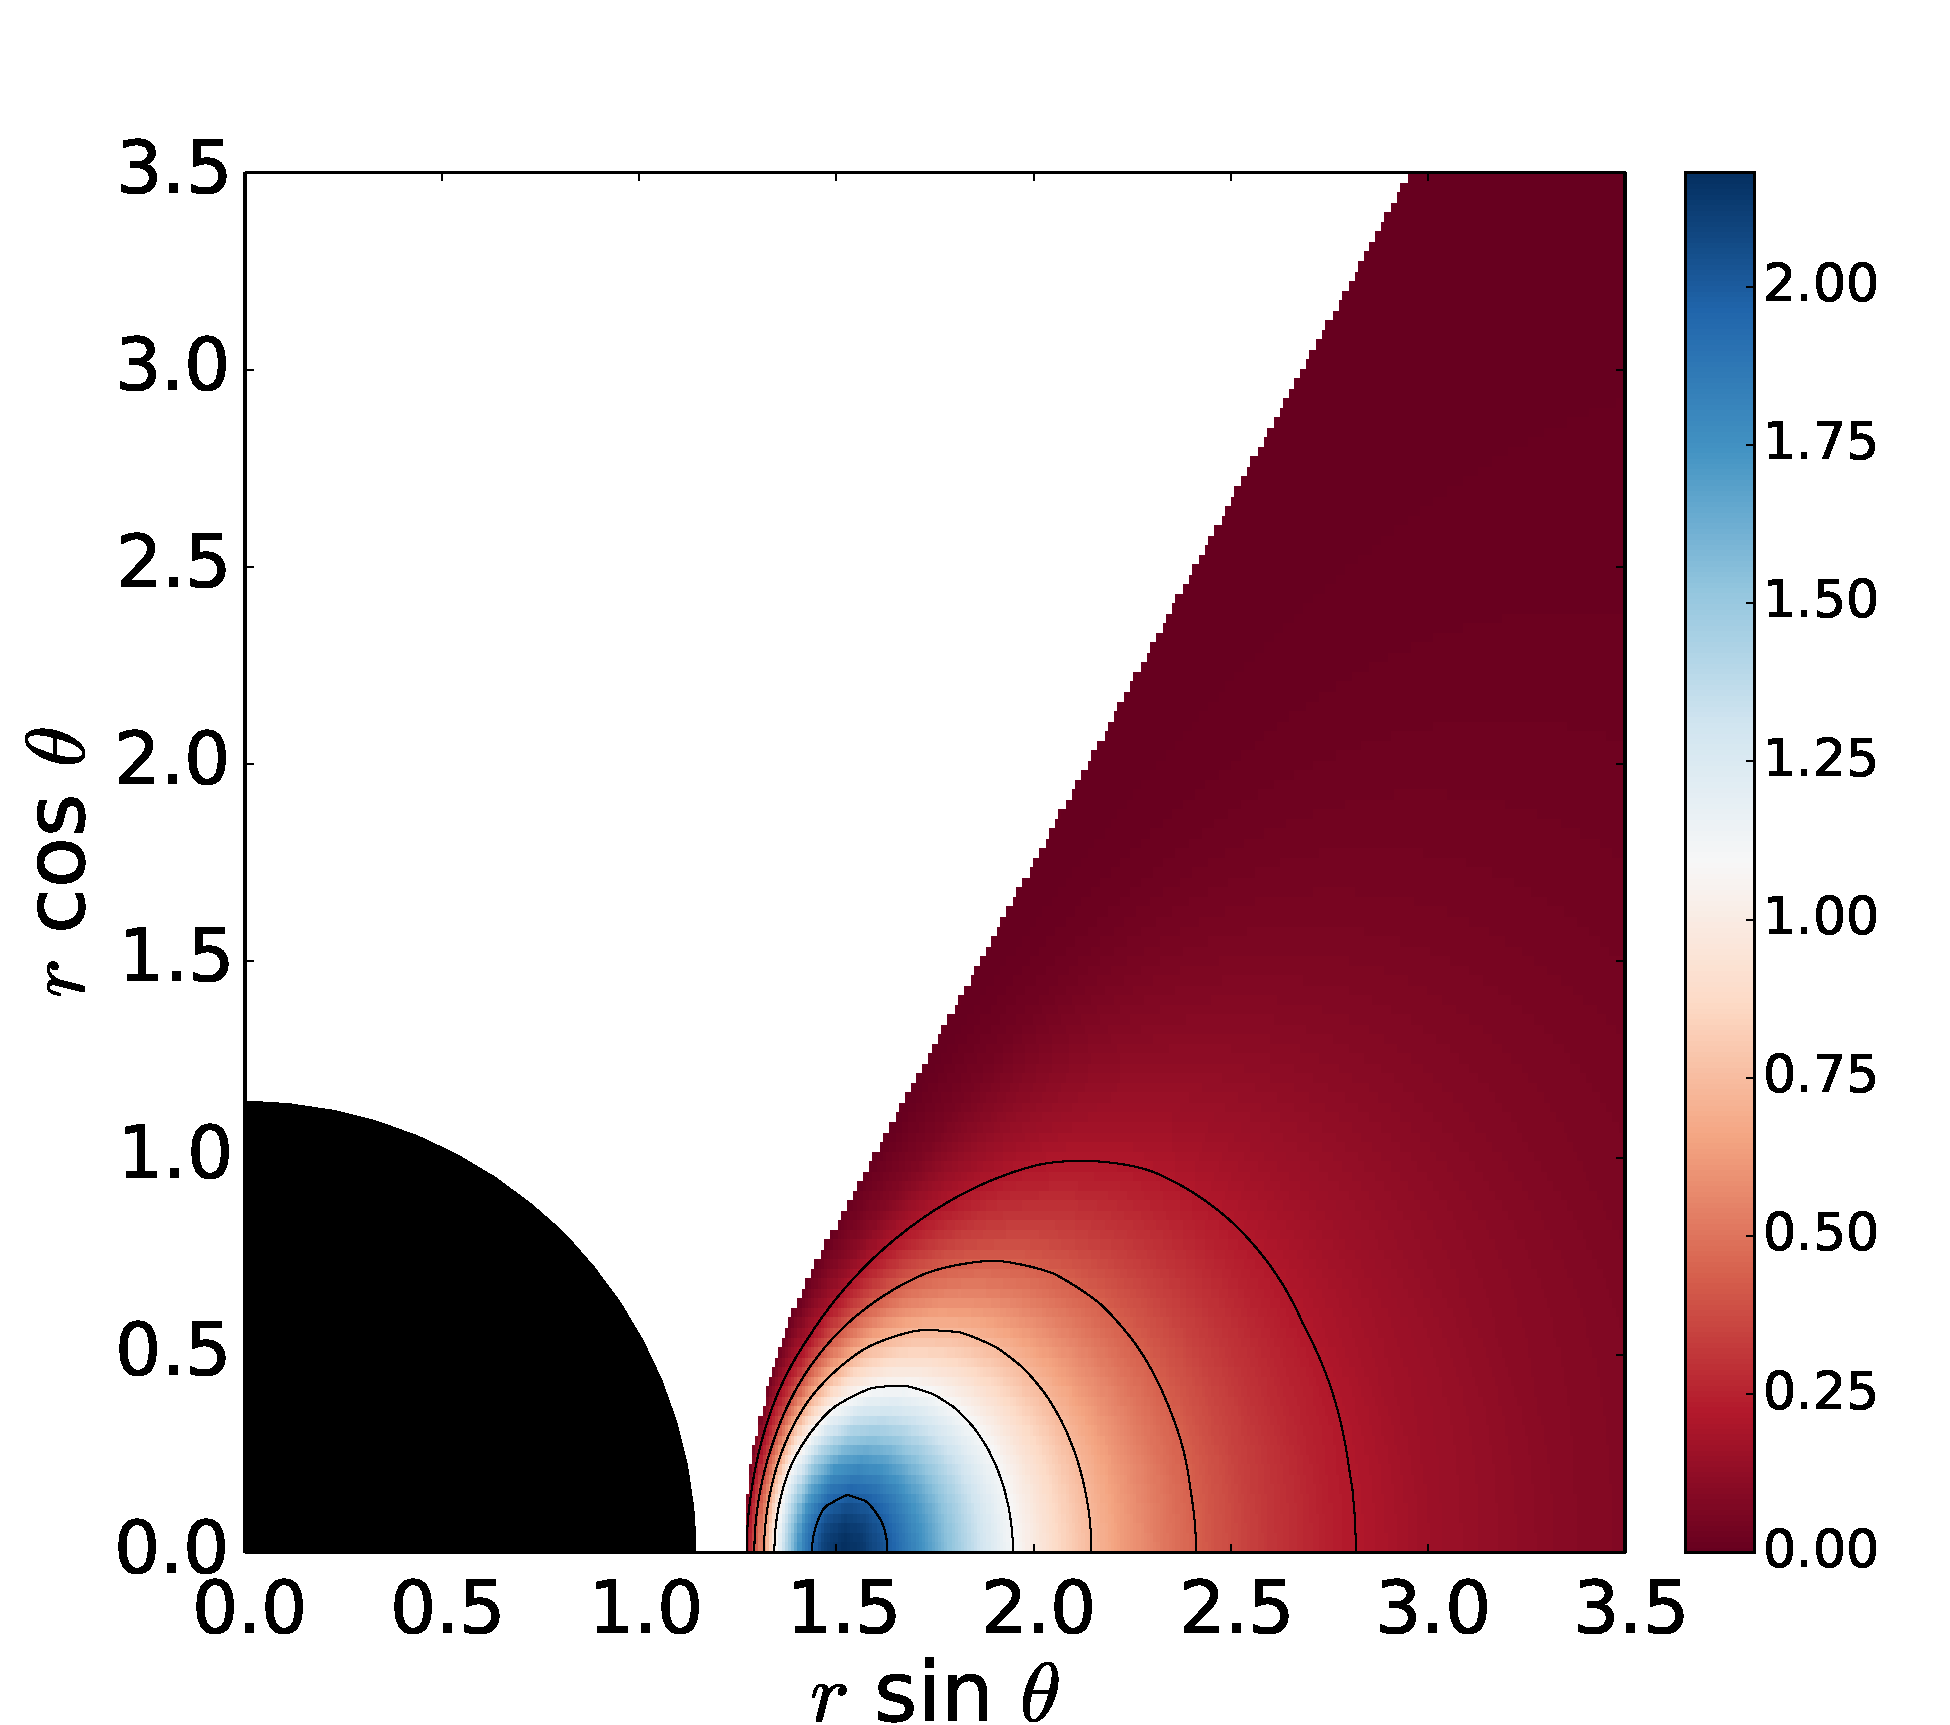
\includegraphics[scale=0.16]{figures/fig2_1_3.pdf}
\\
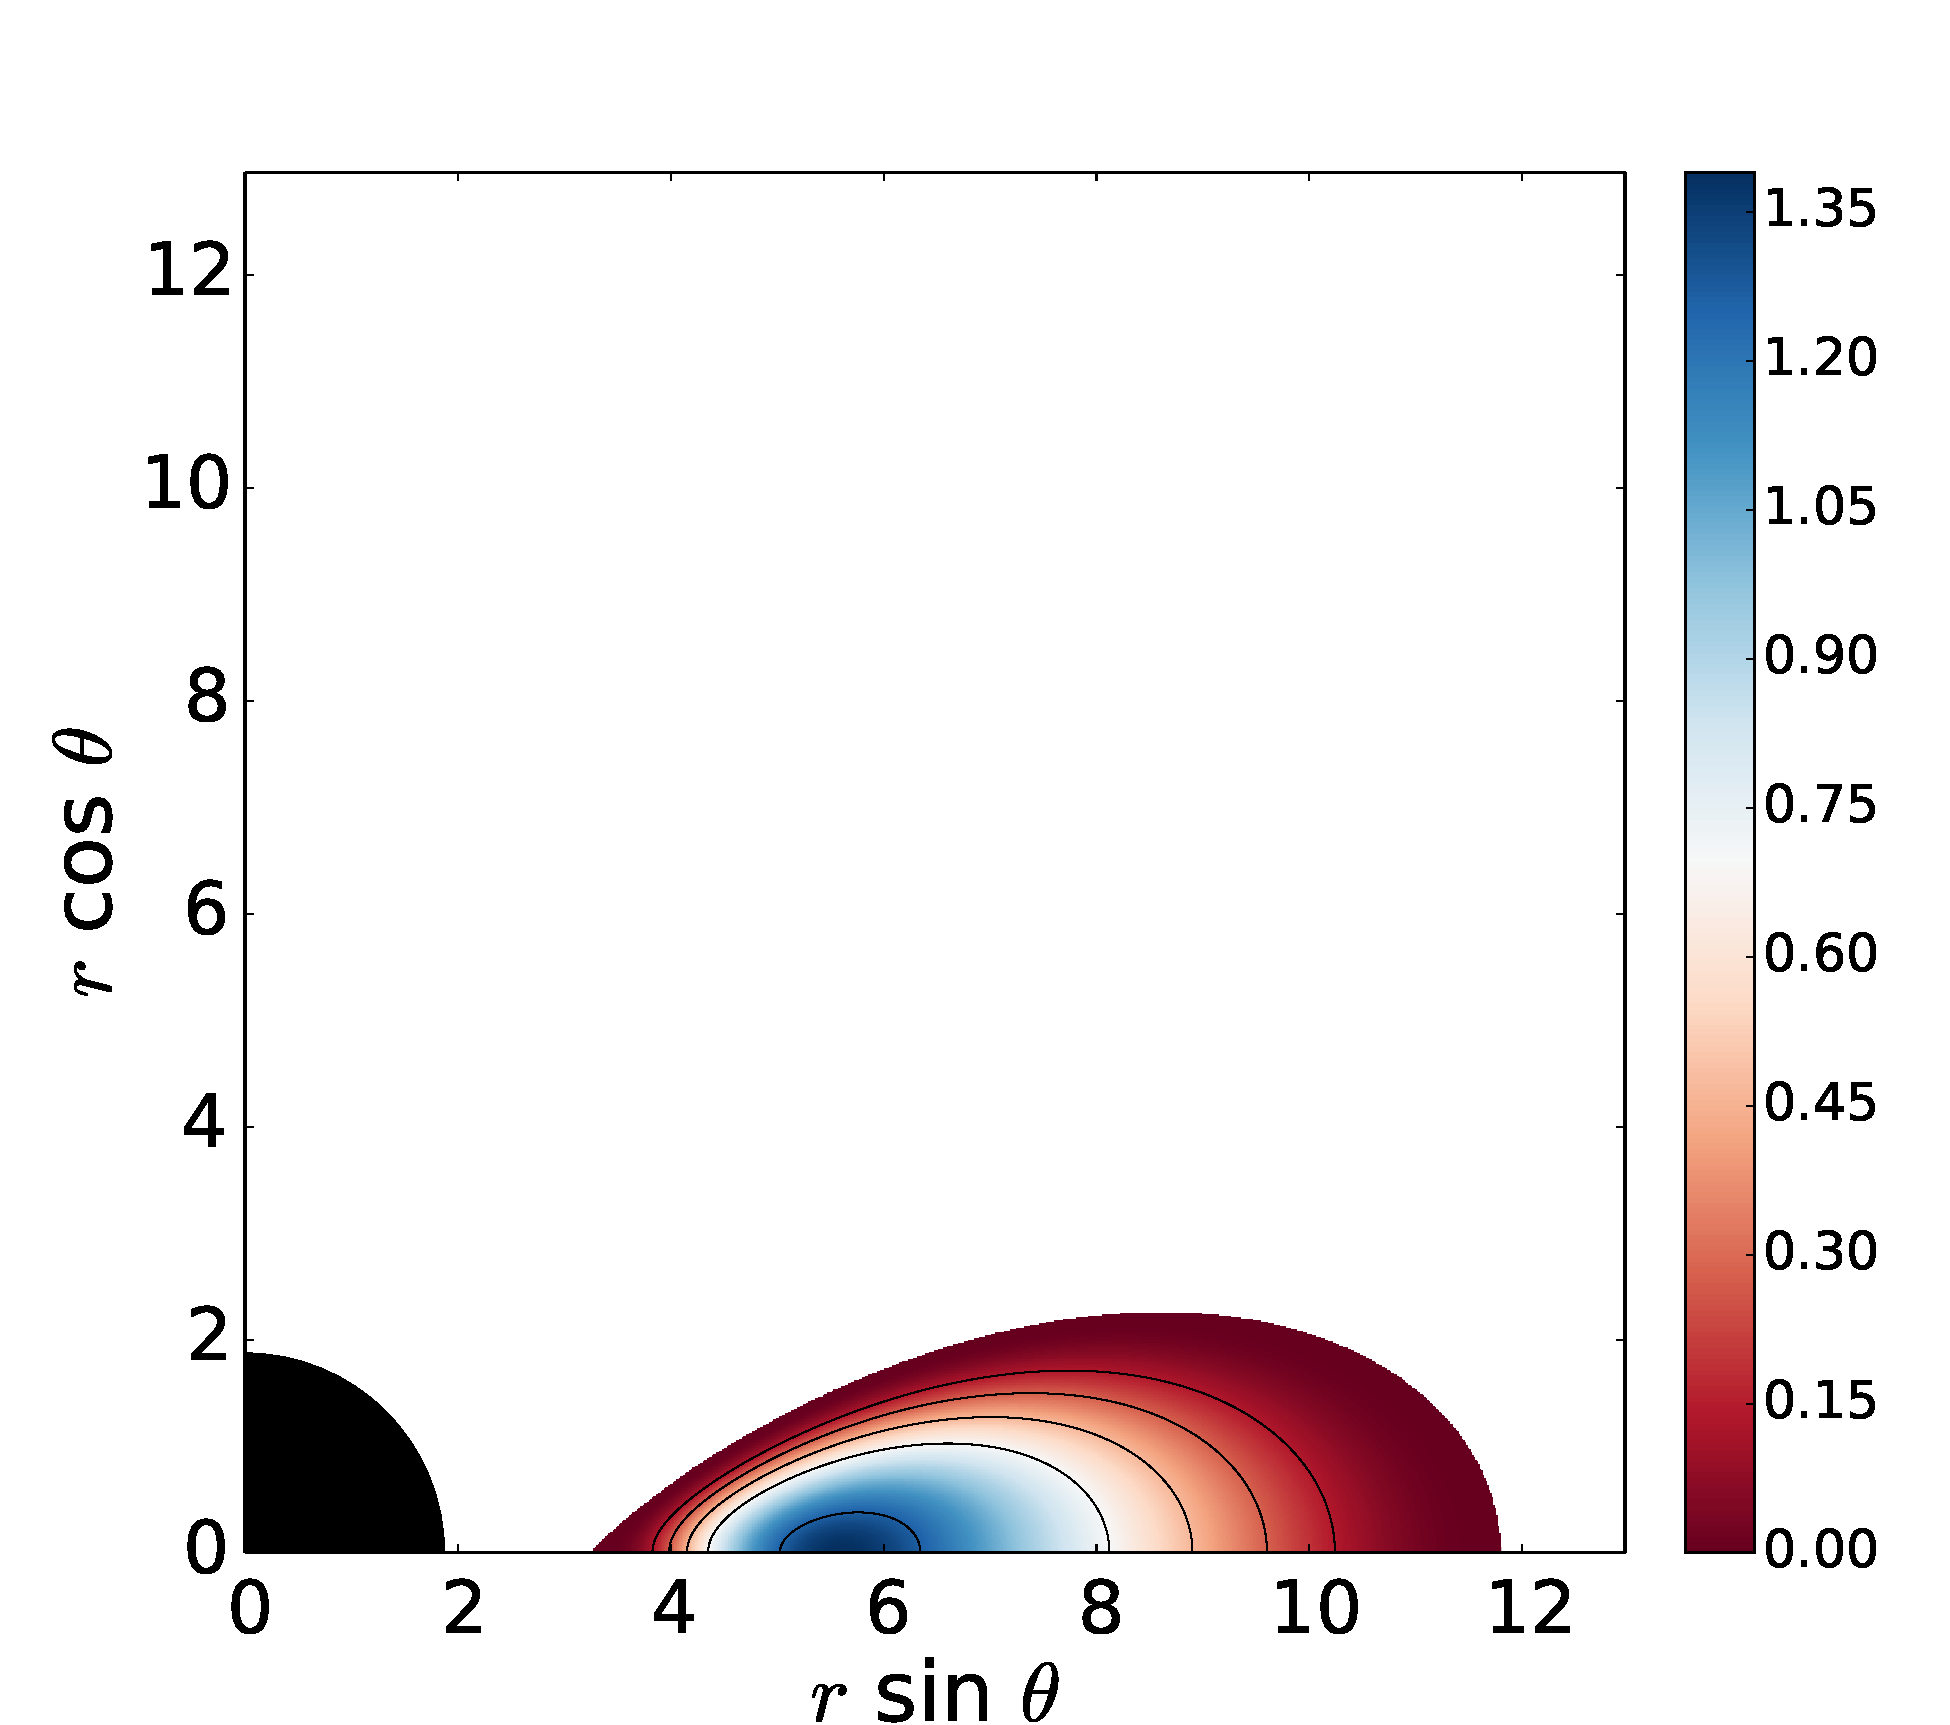
\includegraphics[scale=0.16]{figures/fig2_2_1.pdf}
\hspace{-0.3cm}
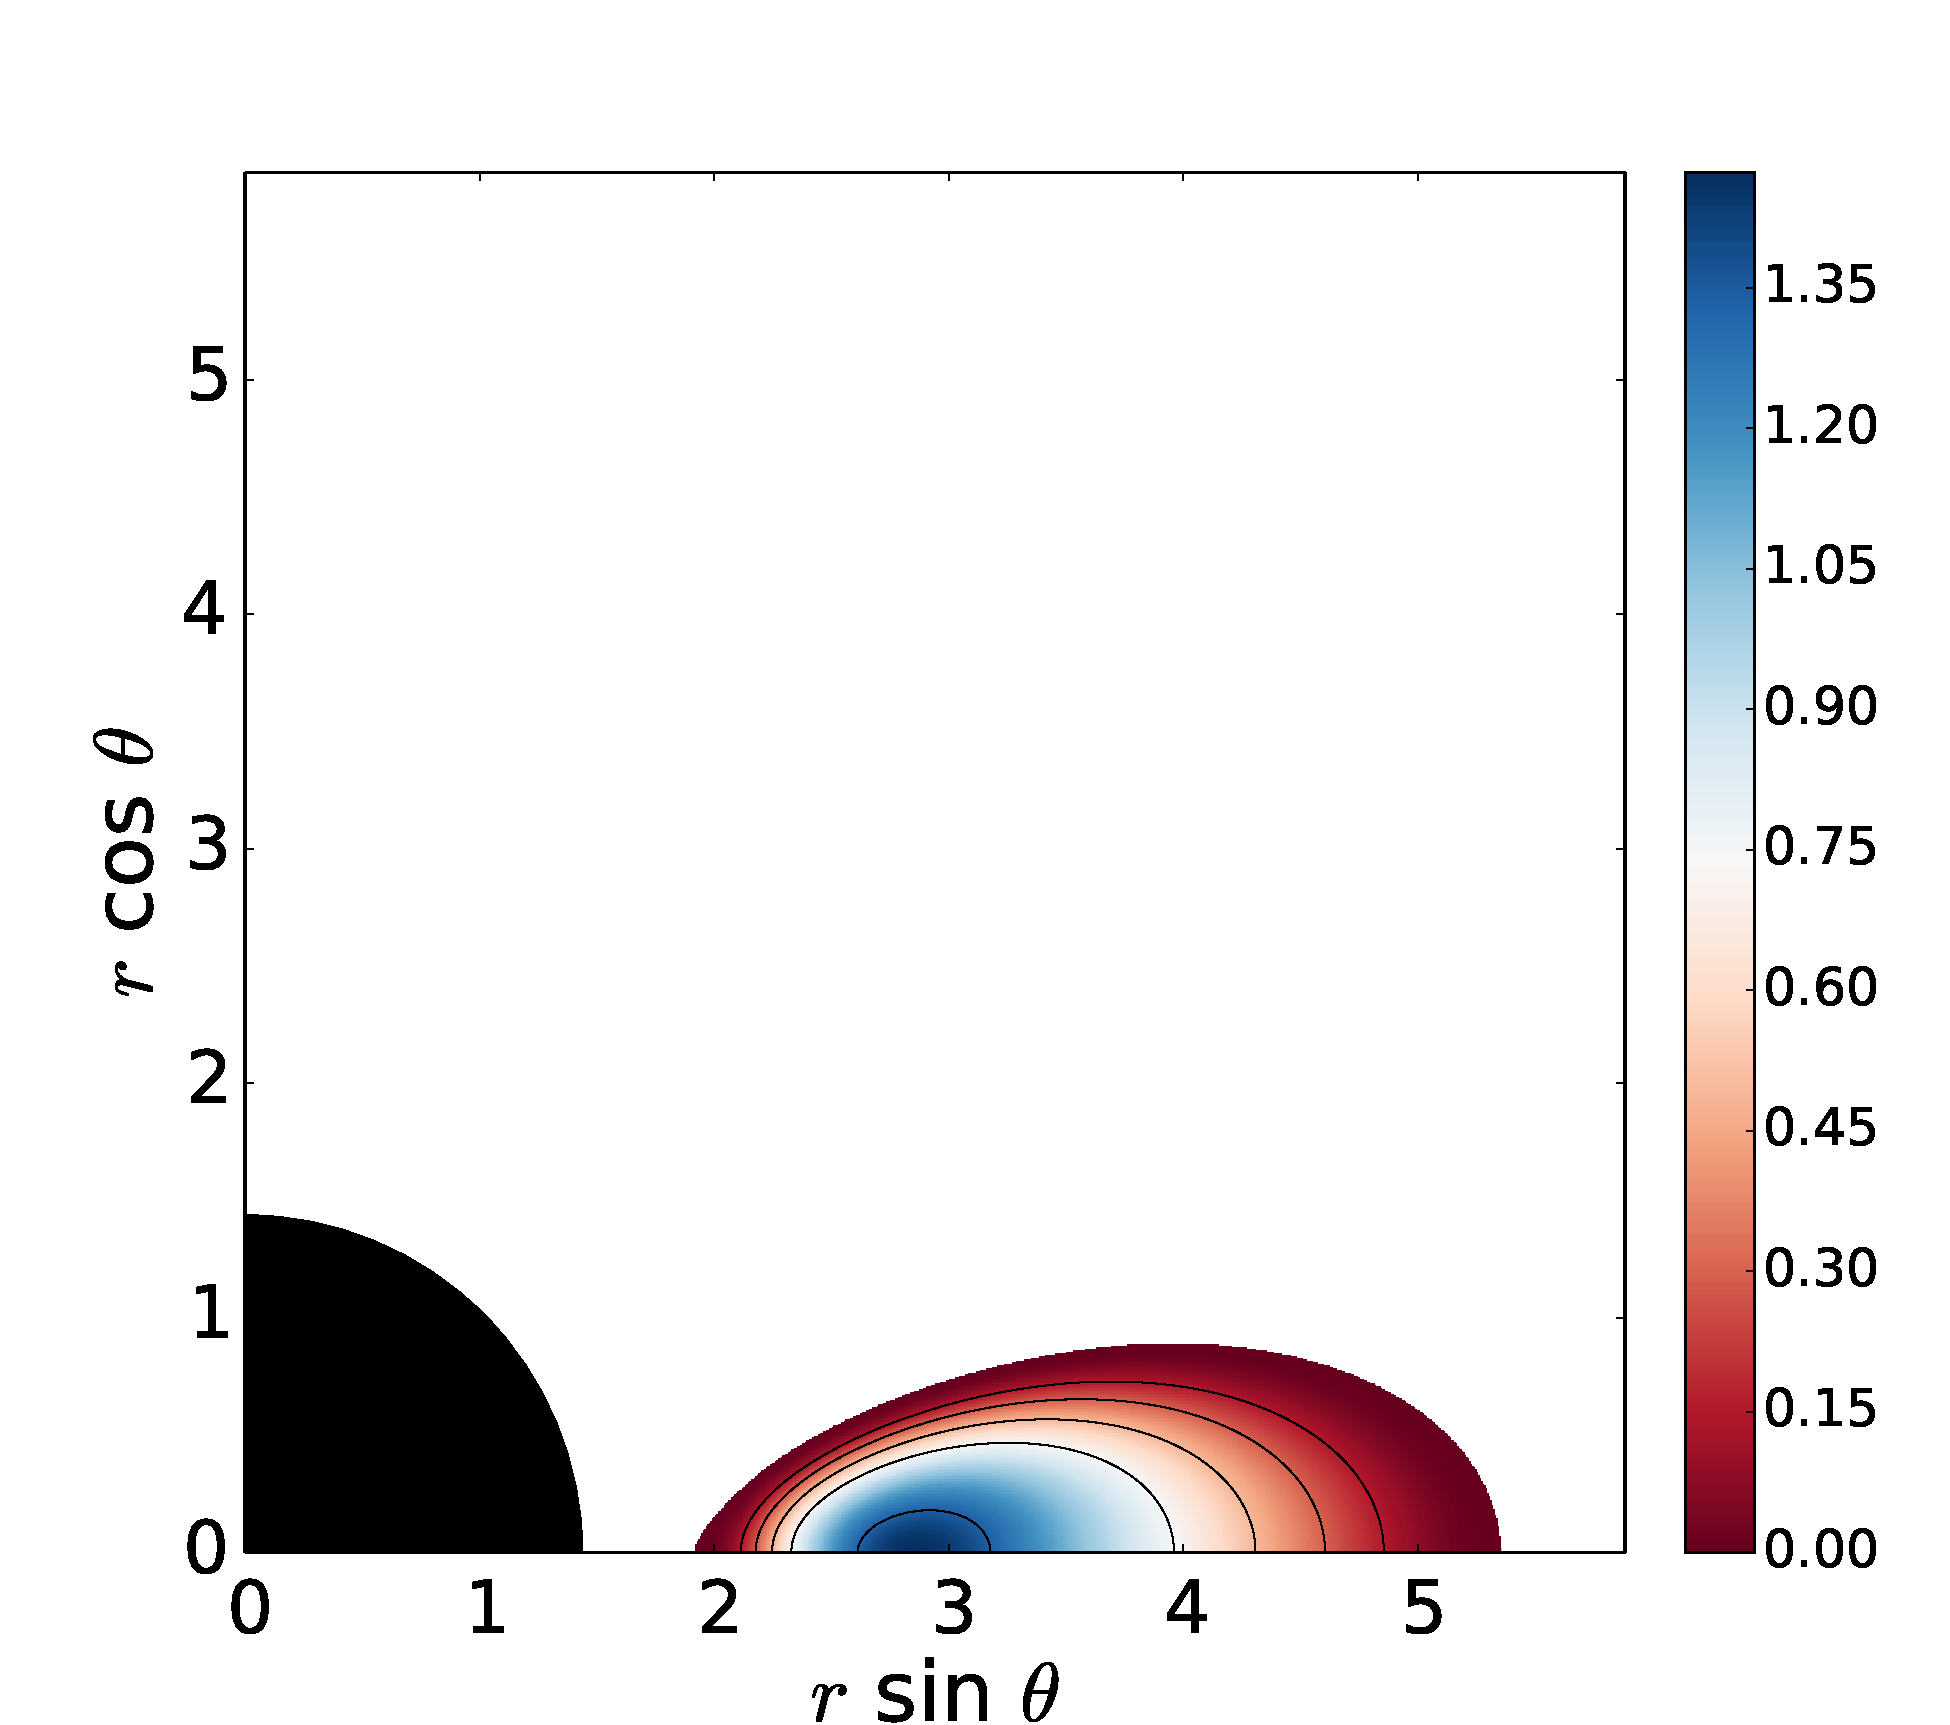
\includegraphics[scale=0.16]{figures/fig2_2_2.pdf}
\hspace{-0.2cm}
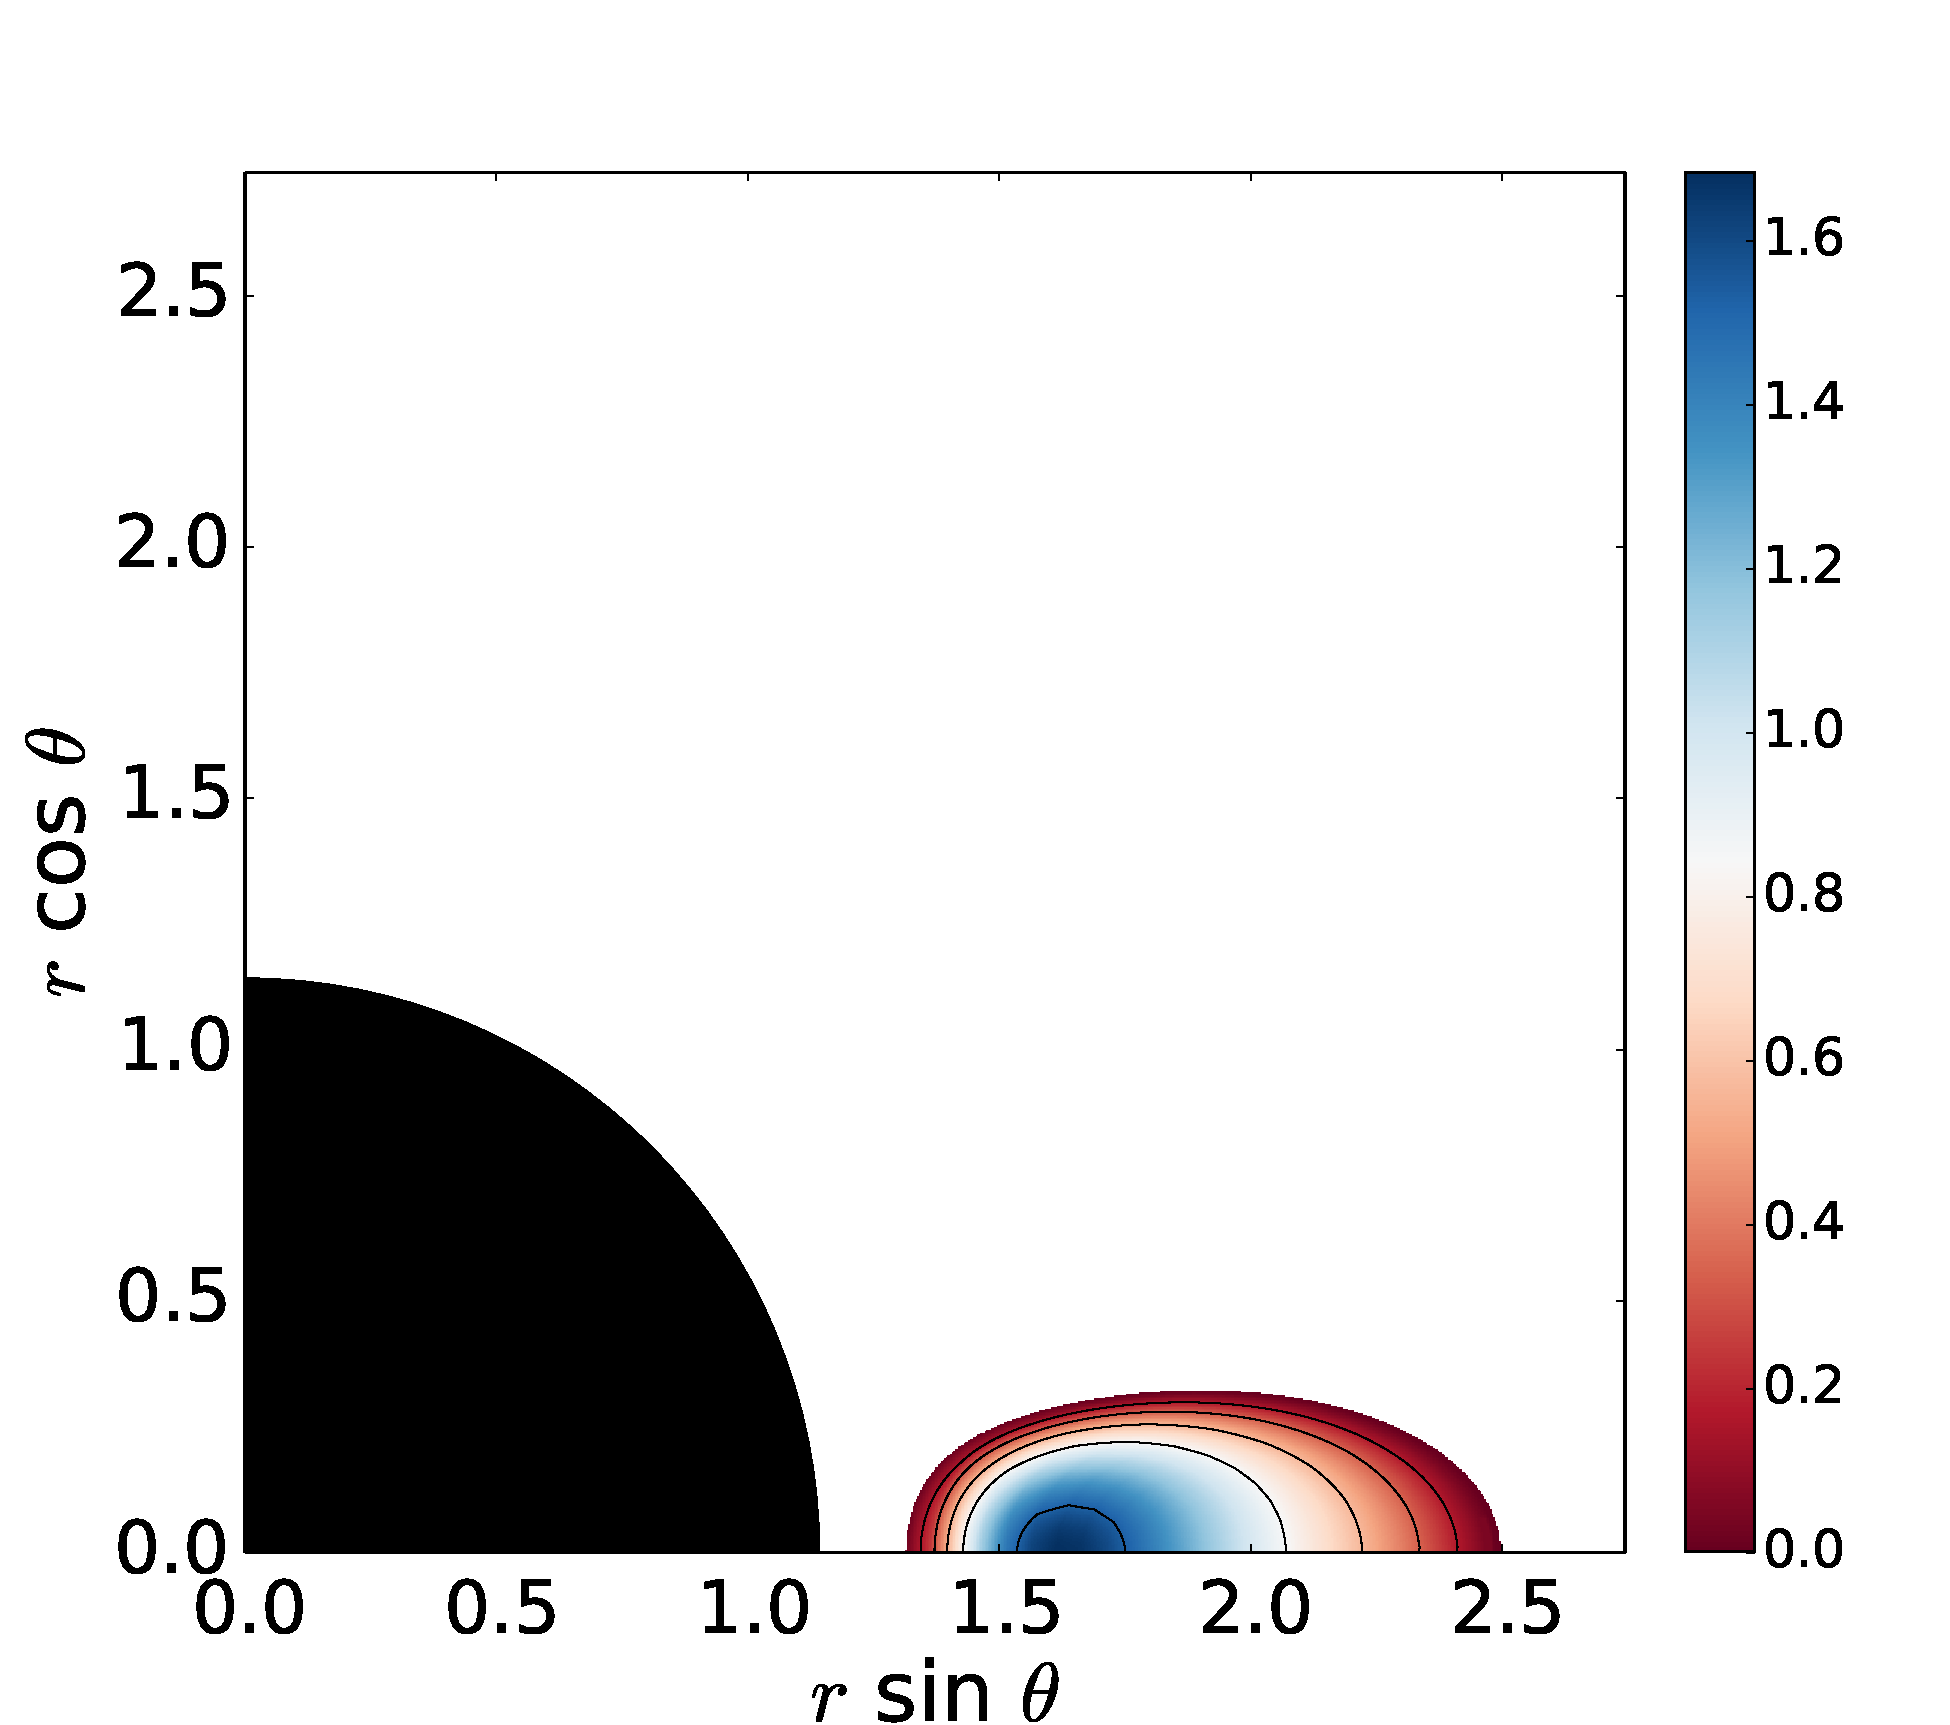
\includegraphics[scale=0.16]{figures/fig2_2_3.pdf}
\\
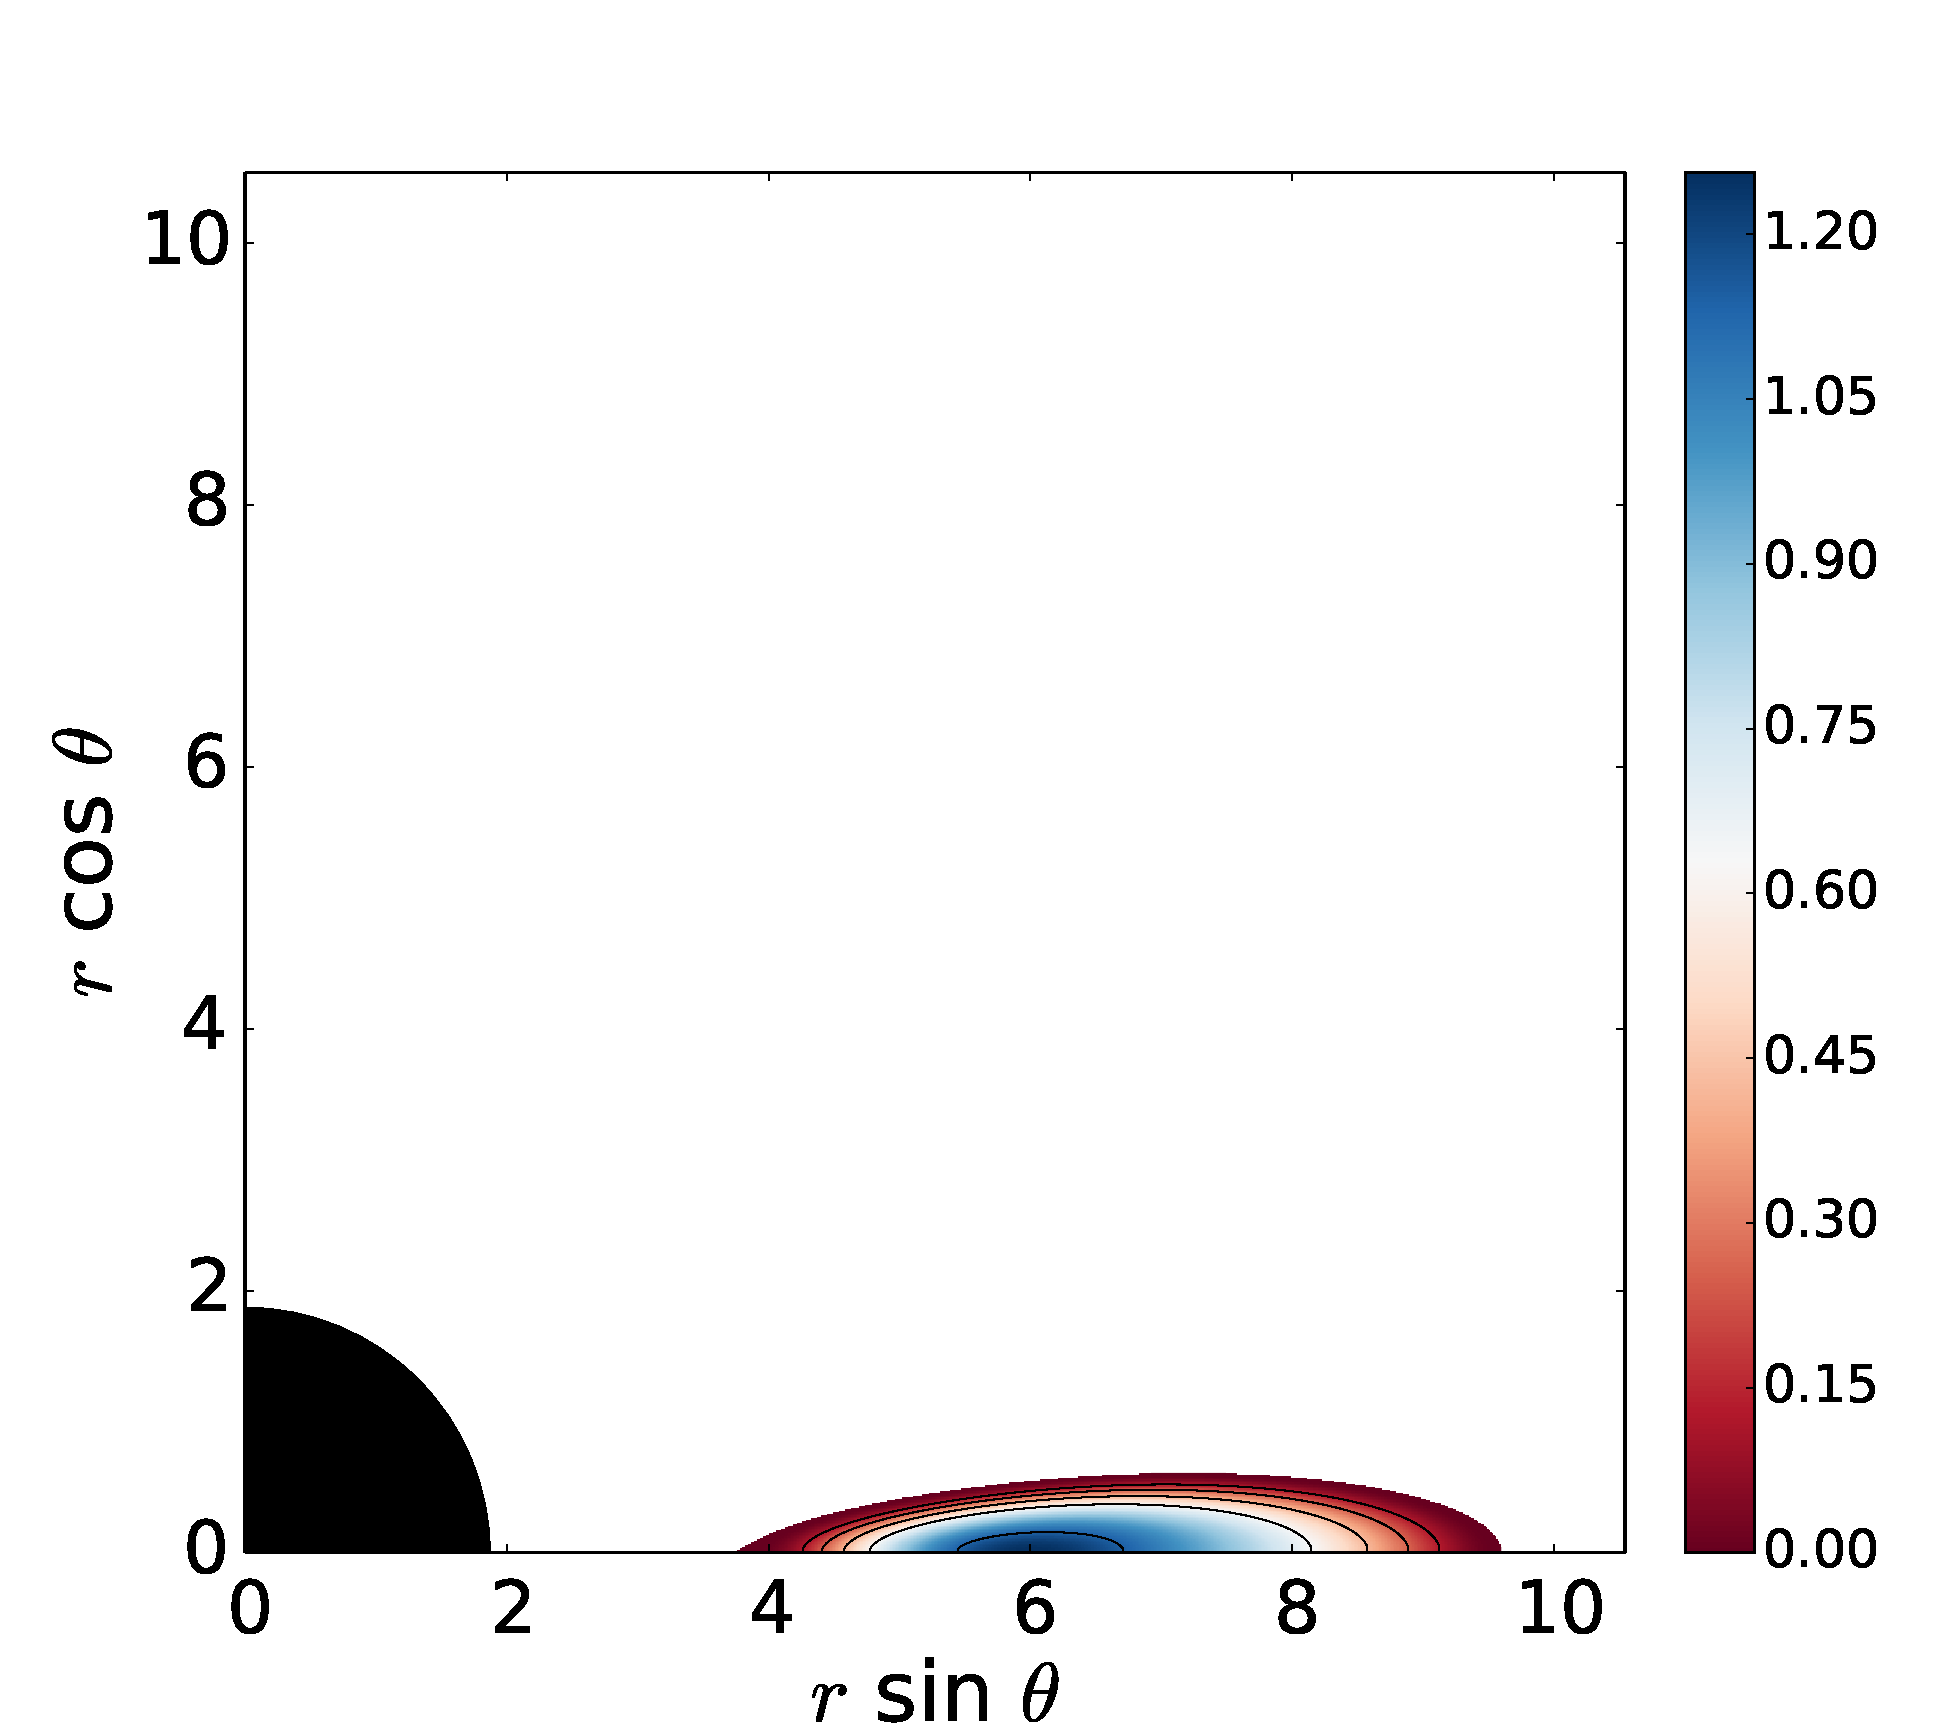
\includegraphics[scale=0.16]{figures/fig2_3_1.pdf}
\hspace{-0.3cm}
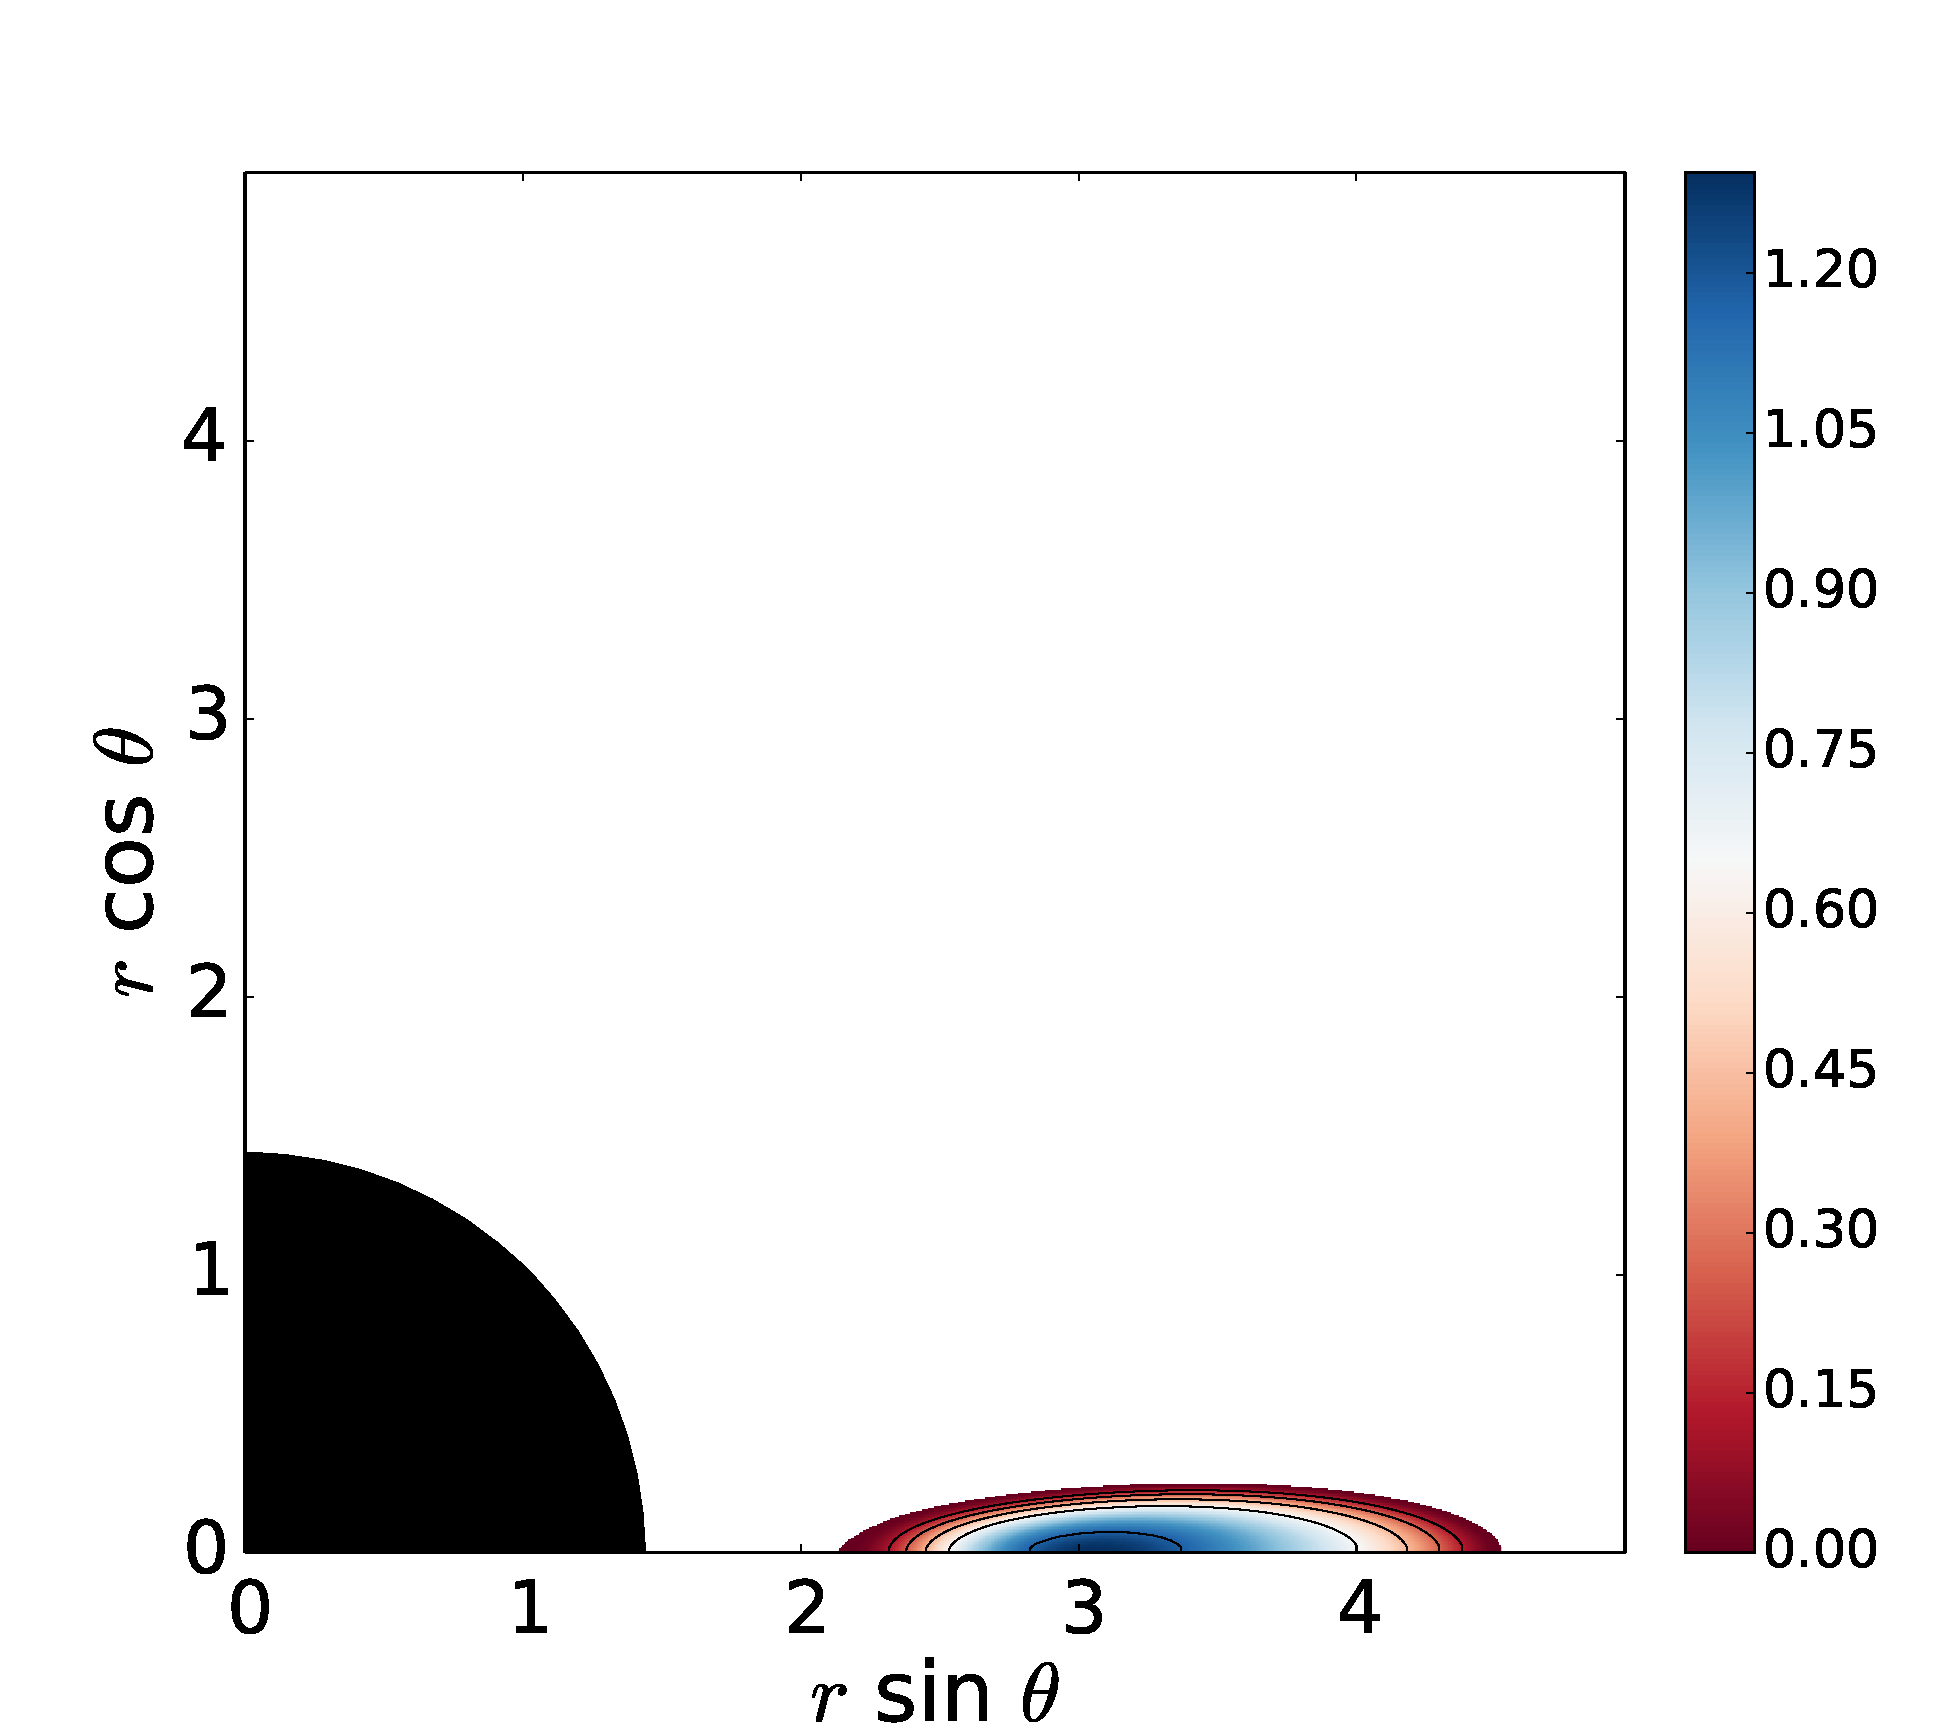
\includegraphics[scale=0.16]{figures/fig2_3_2.pdf}
\hspace{-0.2cm}
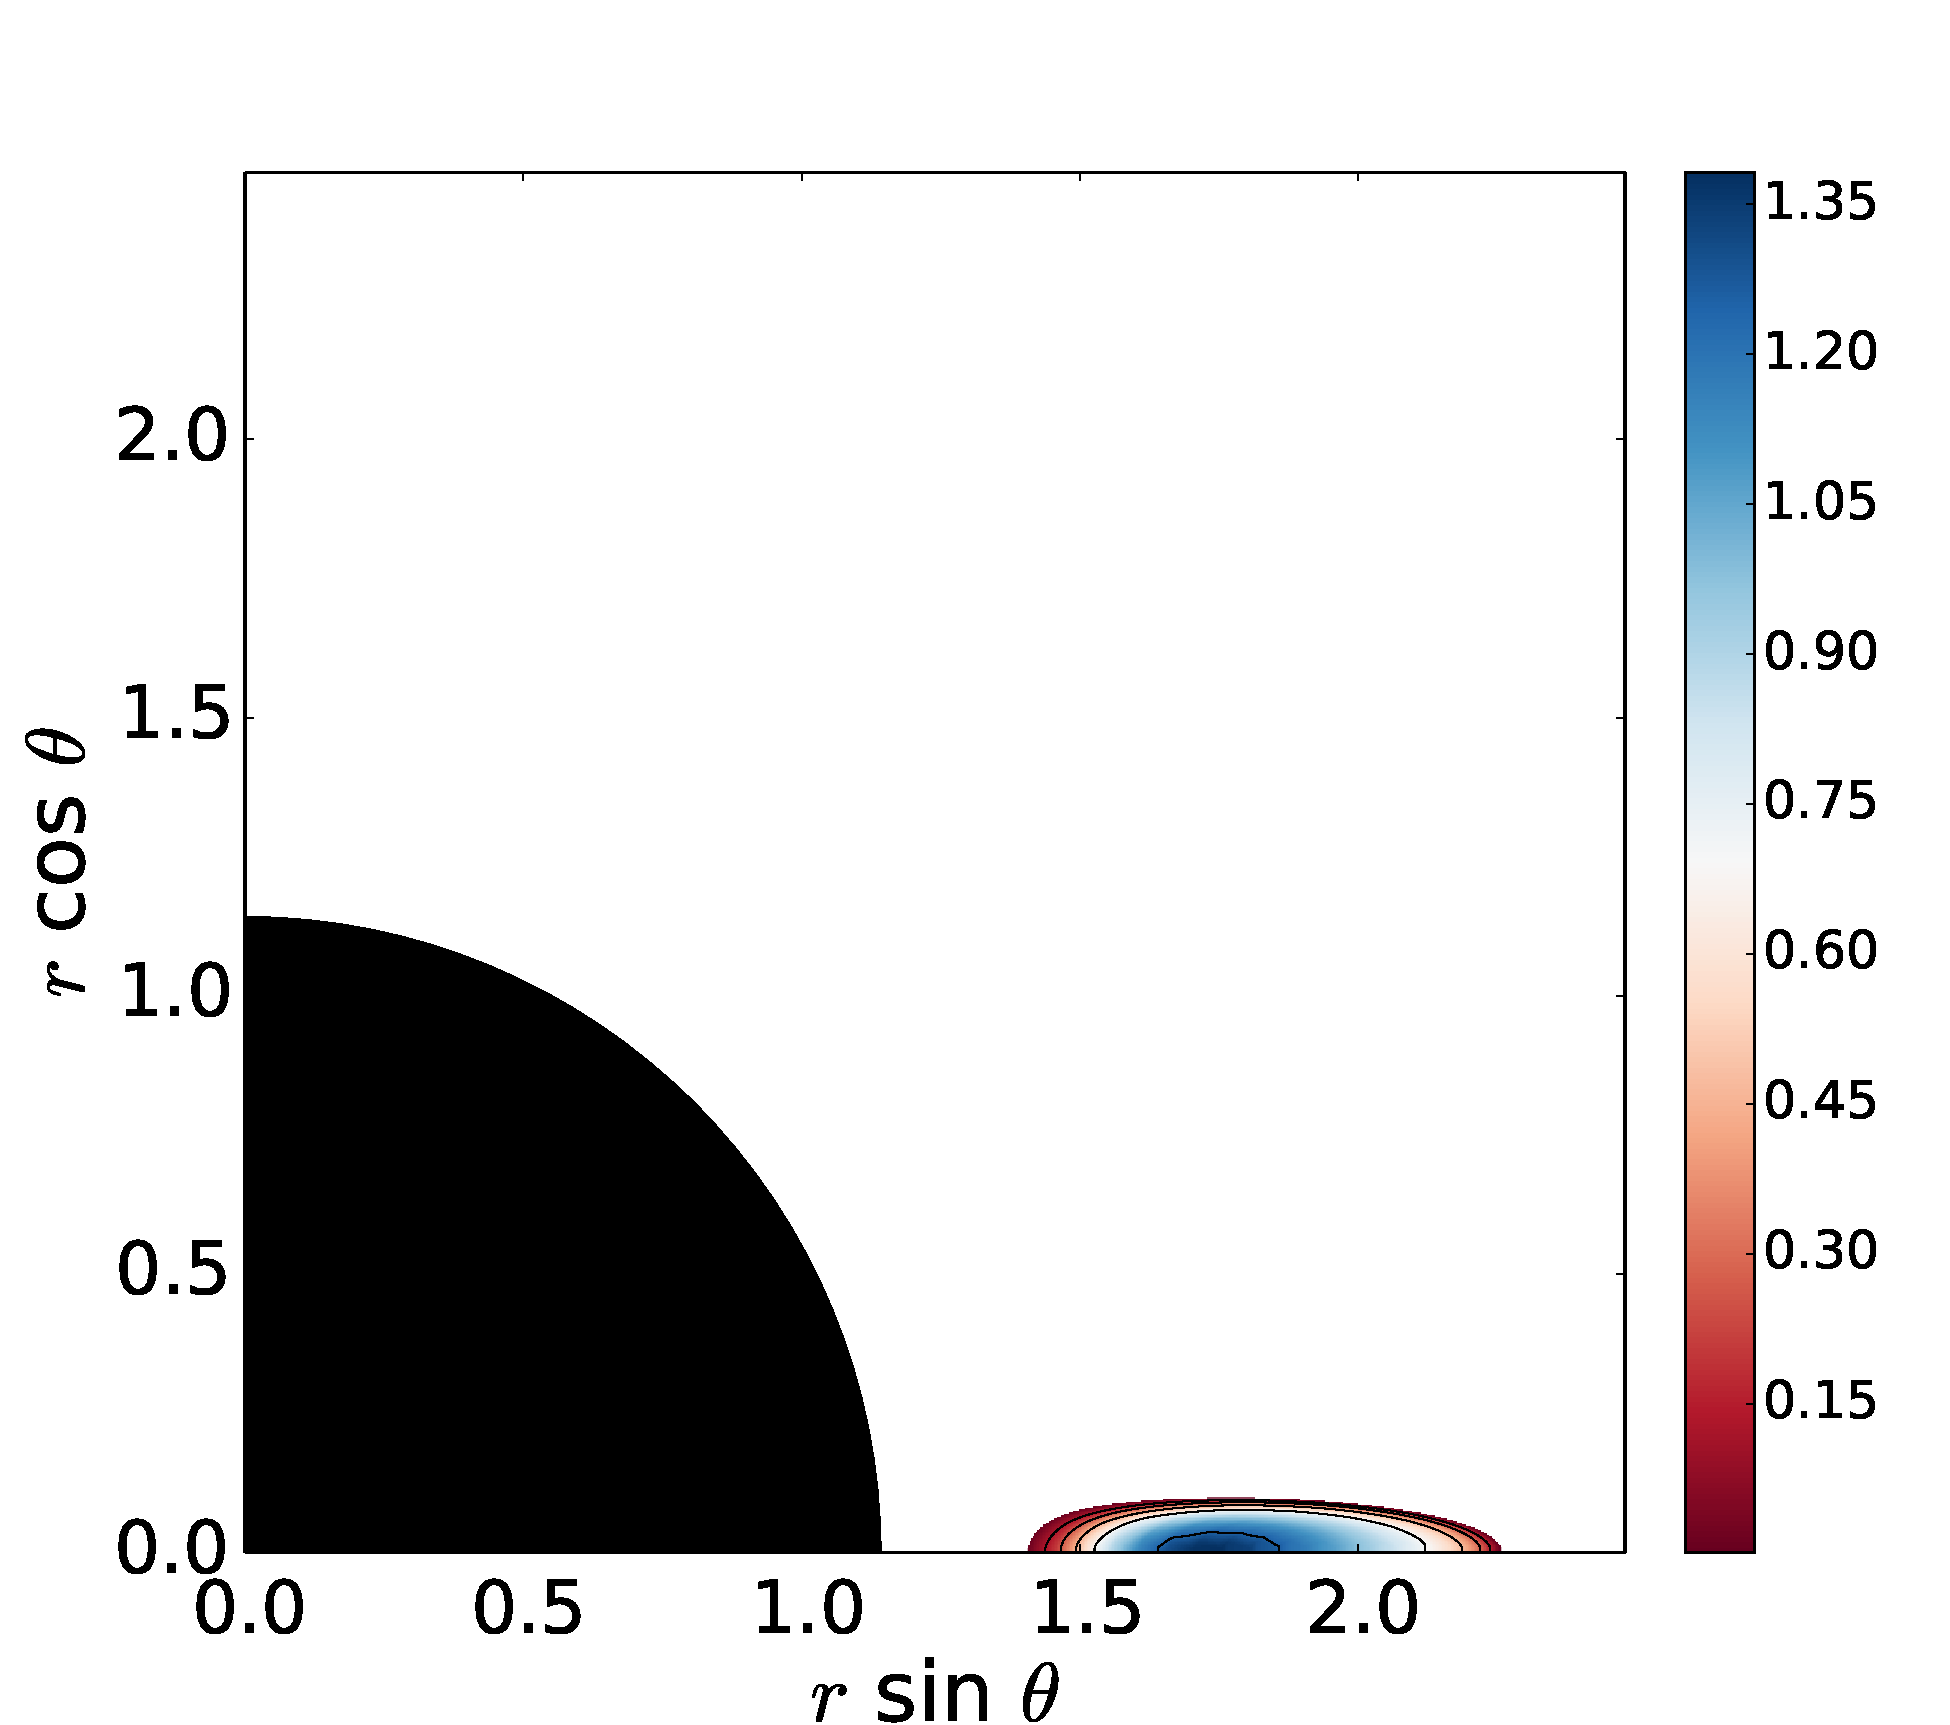
\includegraphics[scale=0.16]{figures/fig2_3_3.pdf}
\\
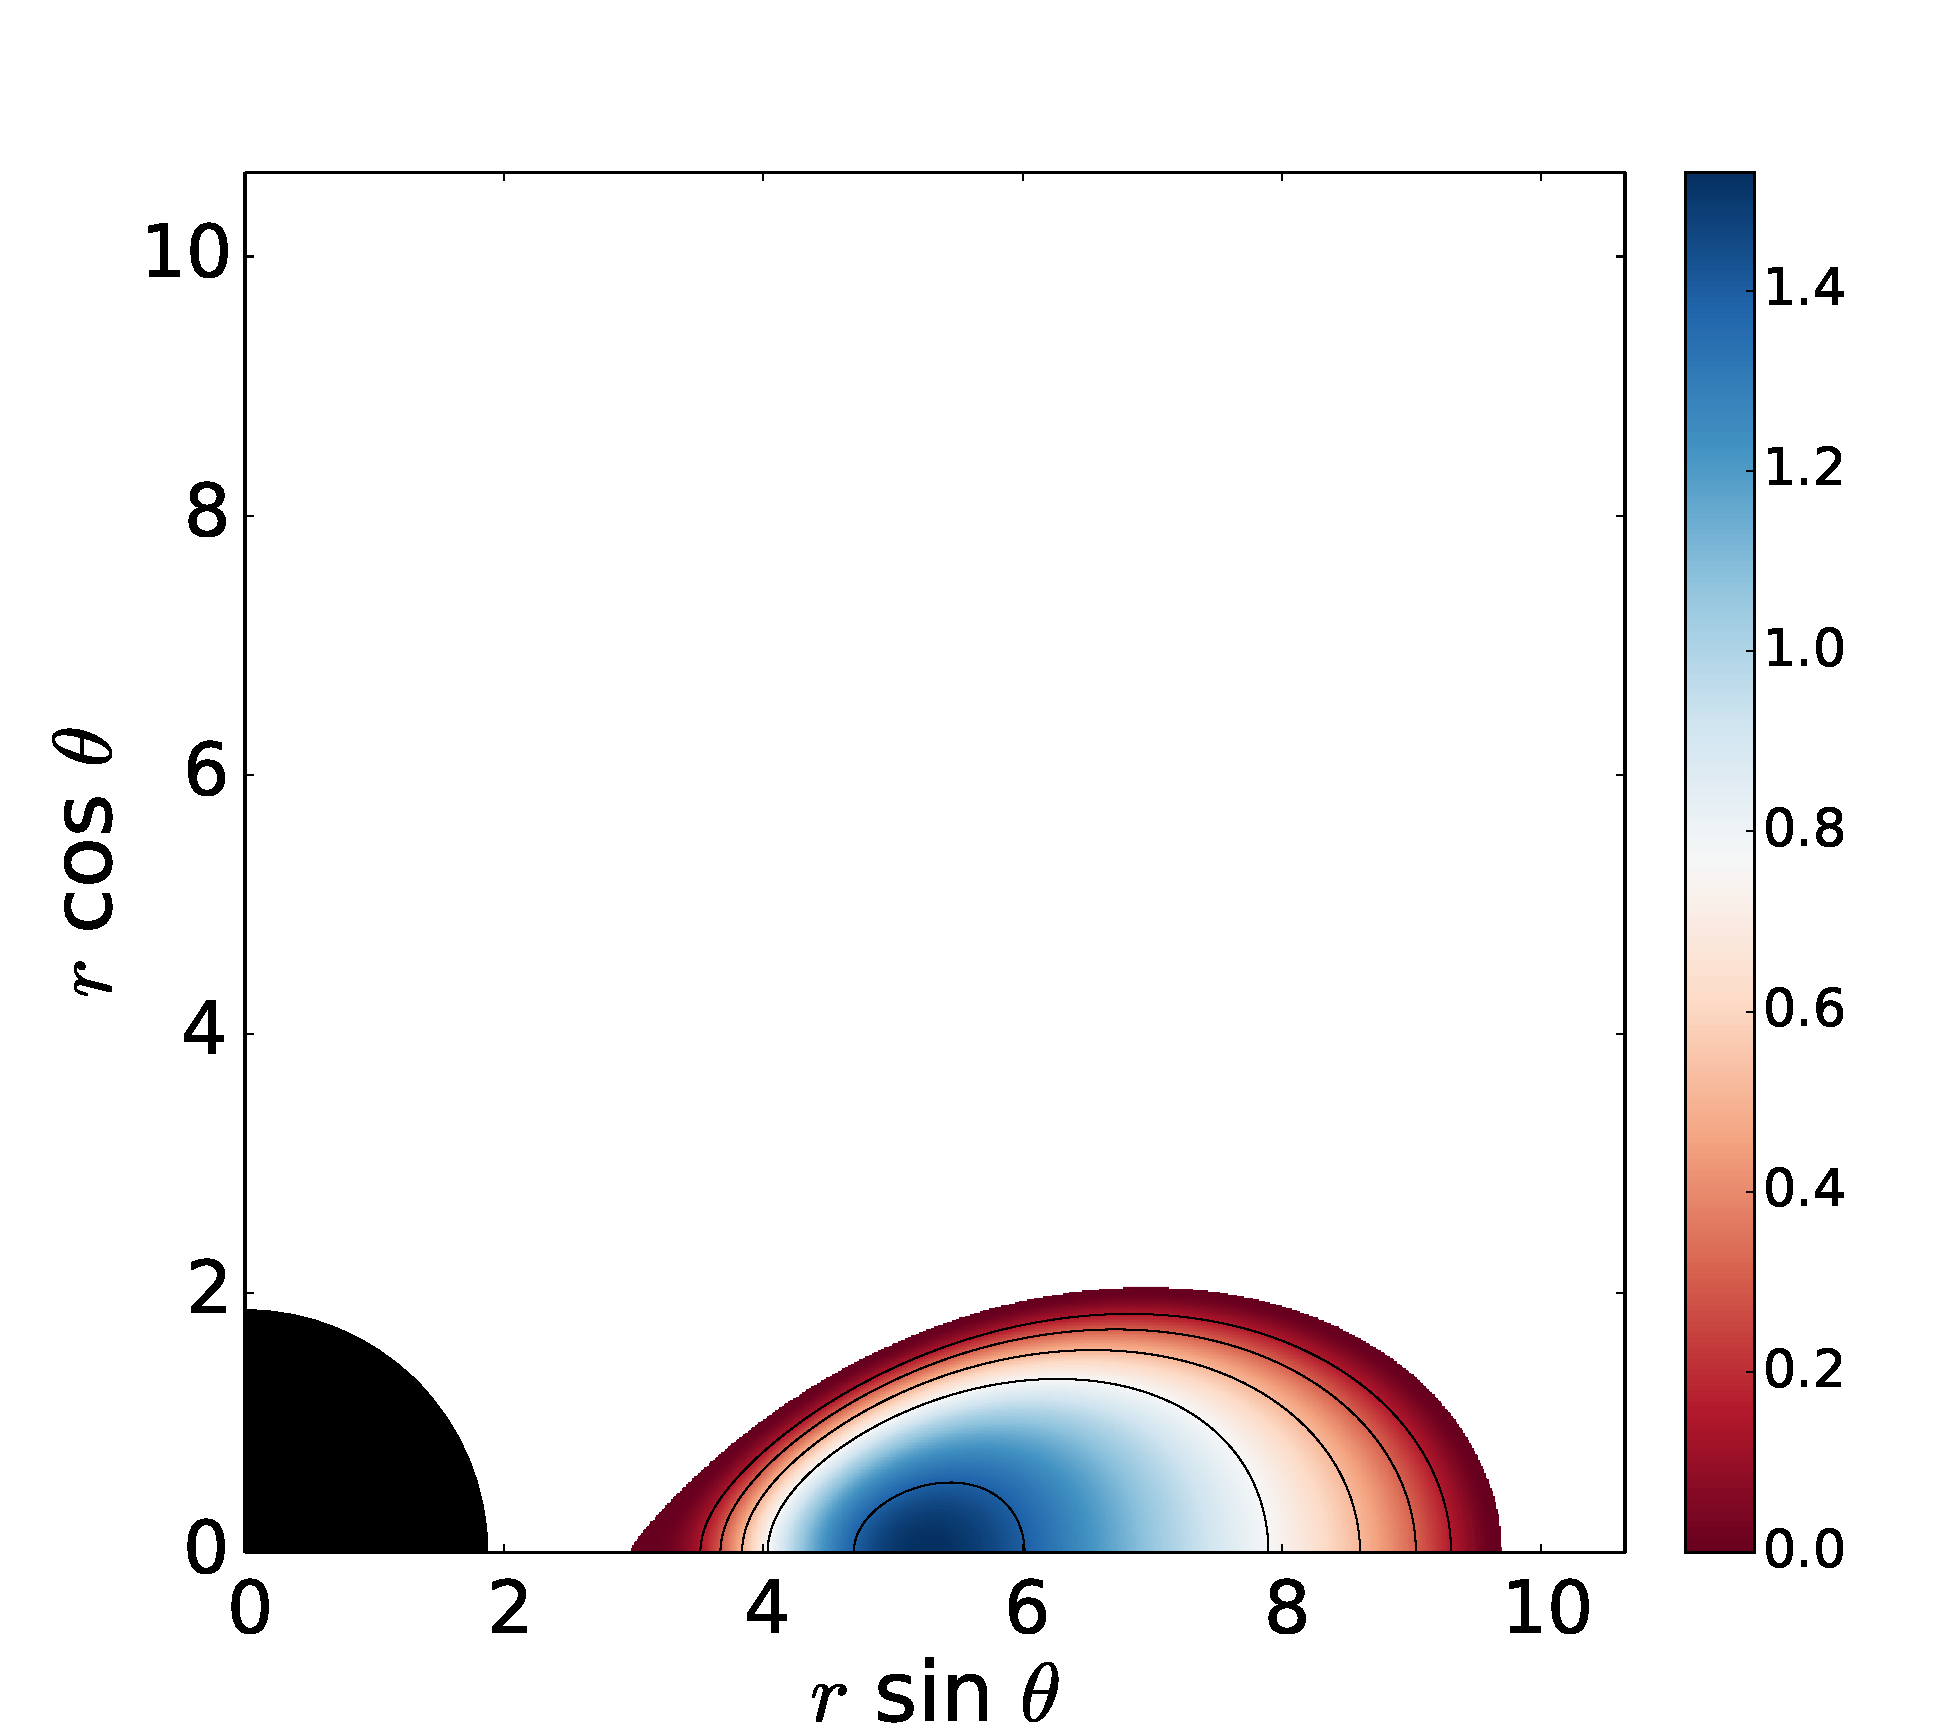
\includegraphics[scale=0.16]{figures/fig2_4_1.pdf}
\hspace{-0.3cm}
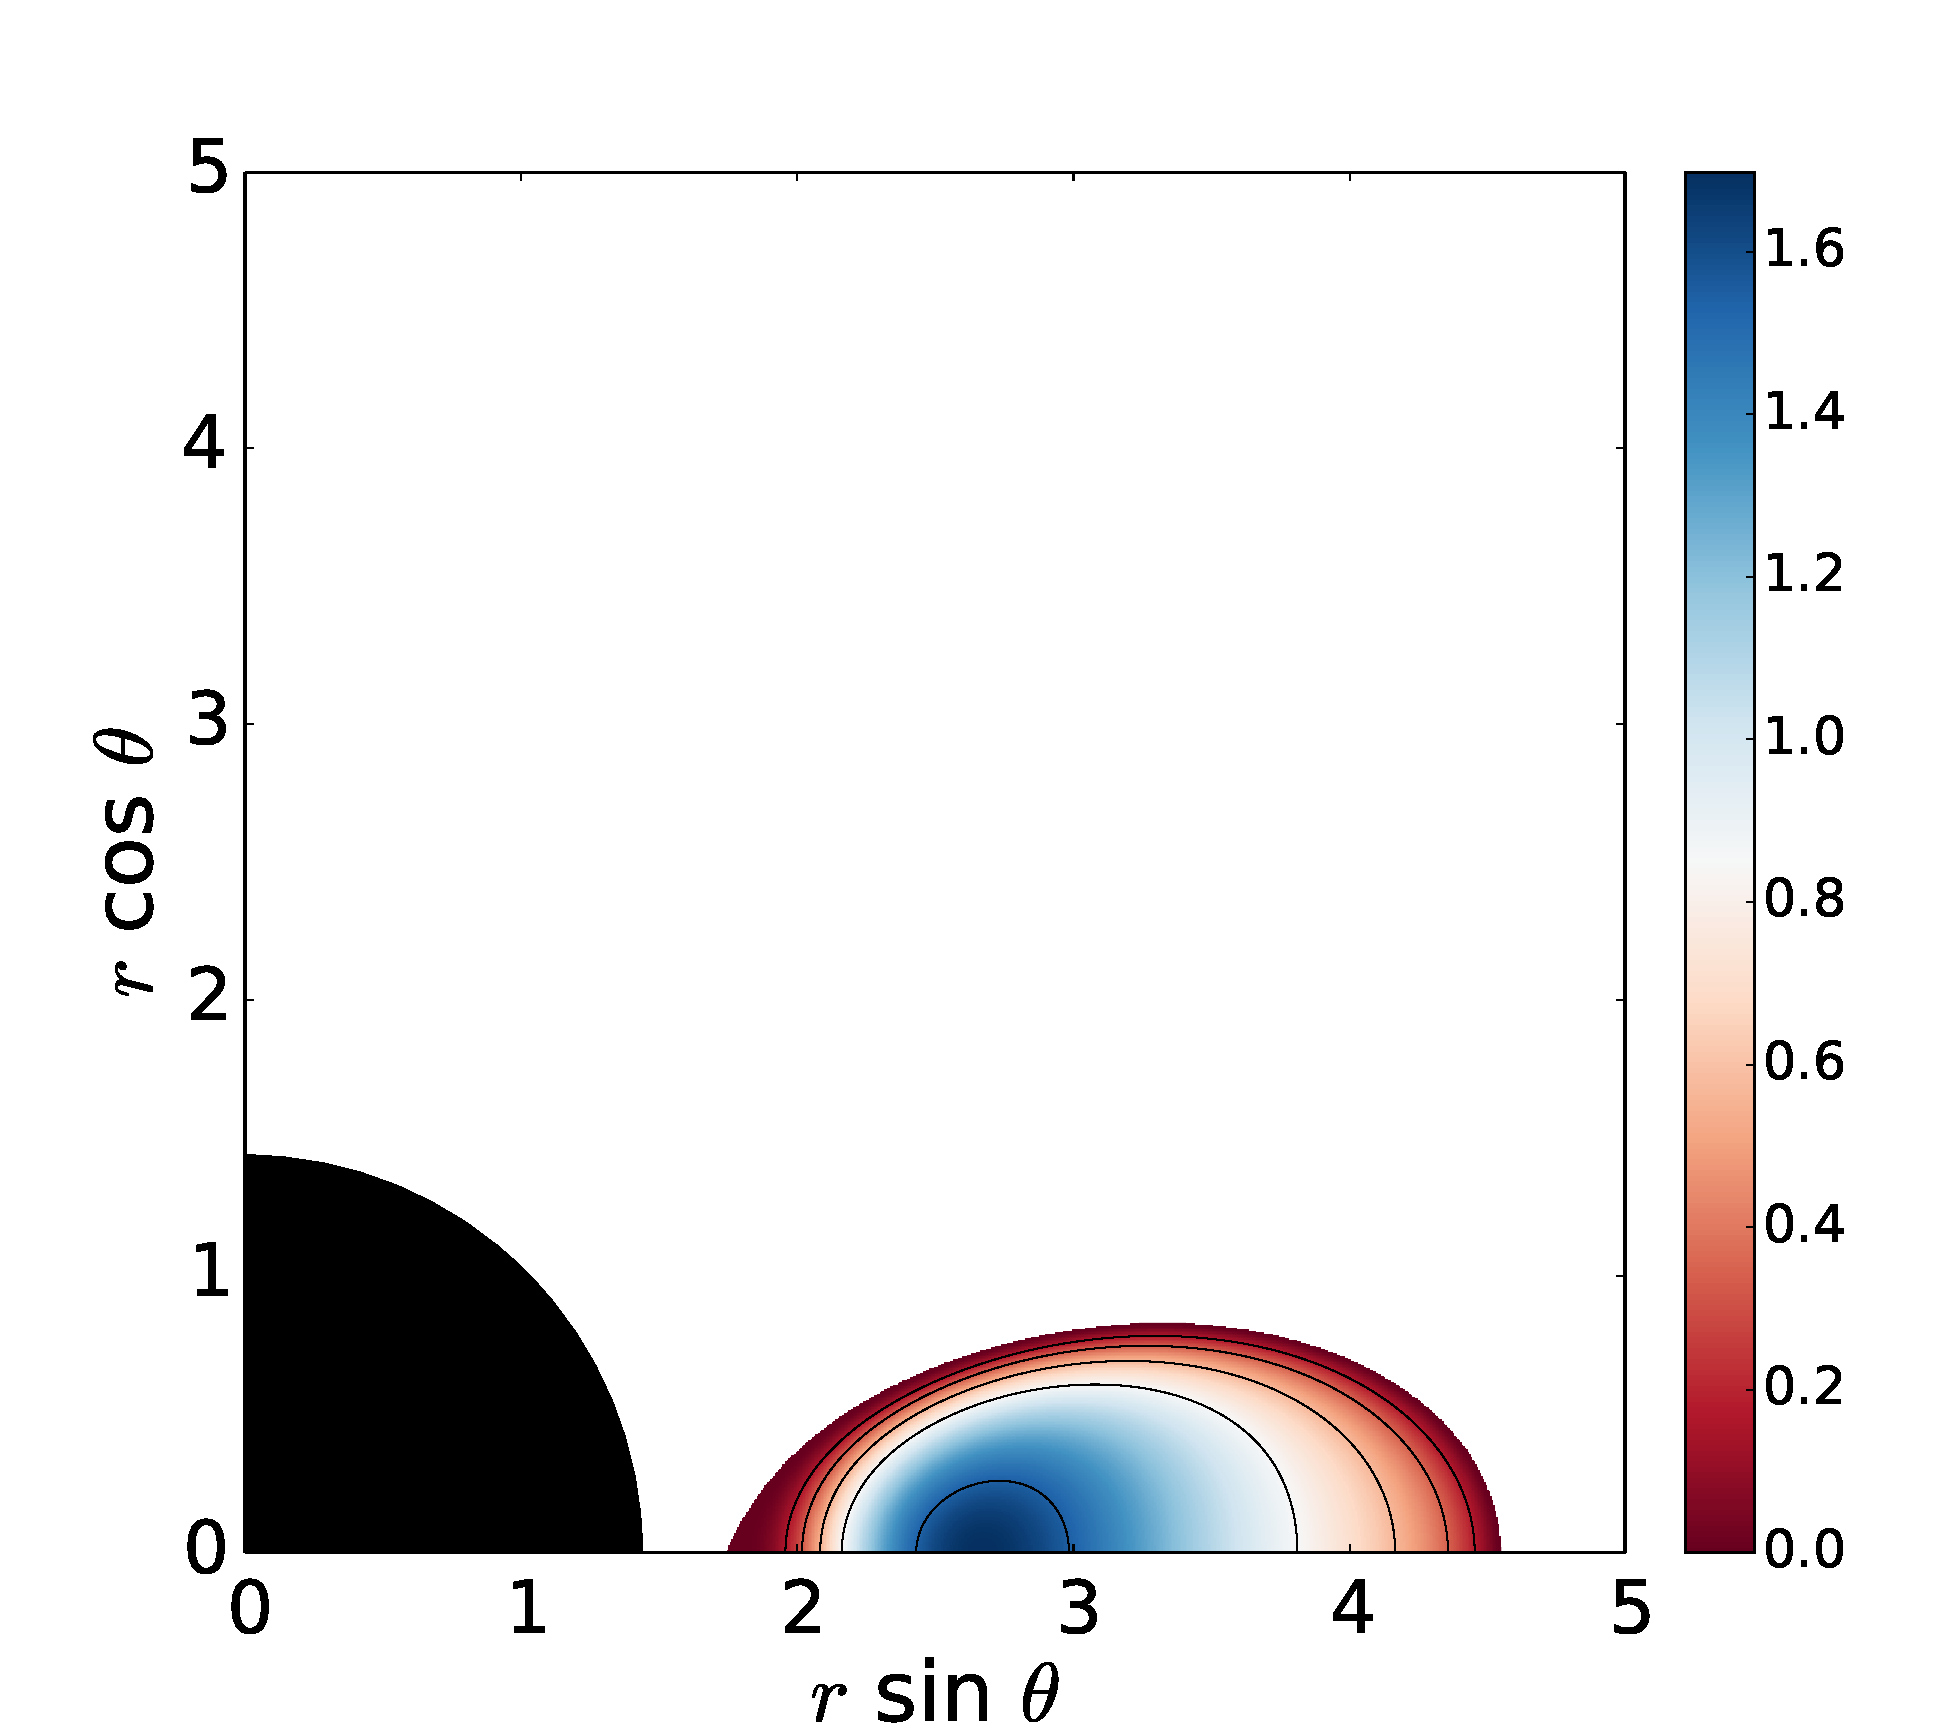
\includegraphics[scale=0.16]{figures/fig2_4_2.pdf}
\hspace{-0.2cm}
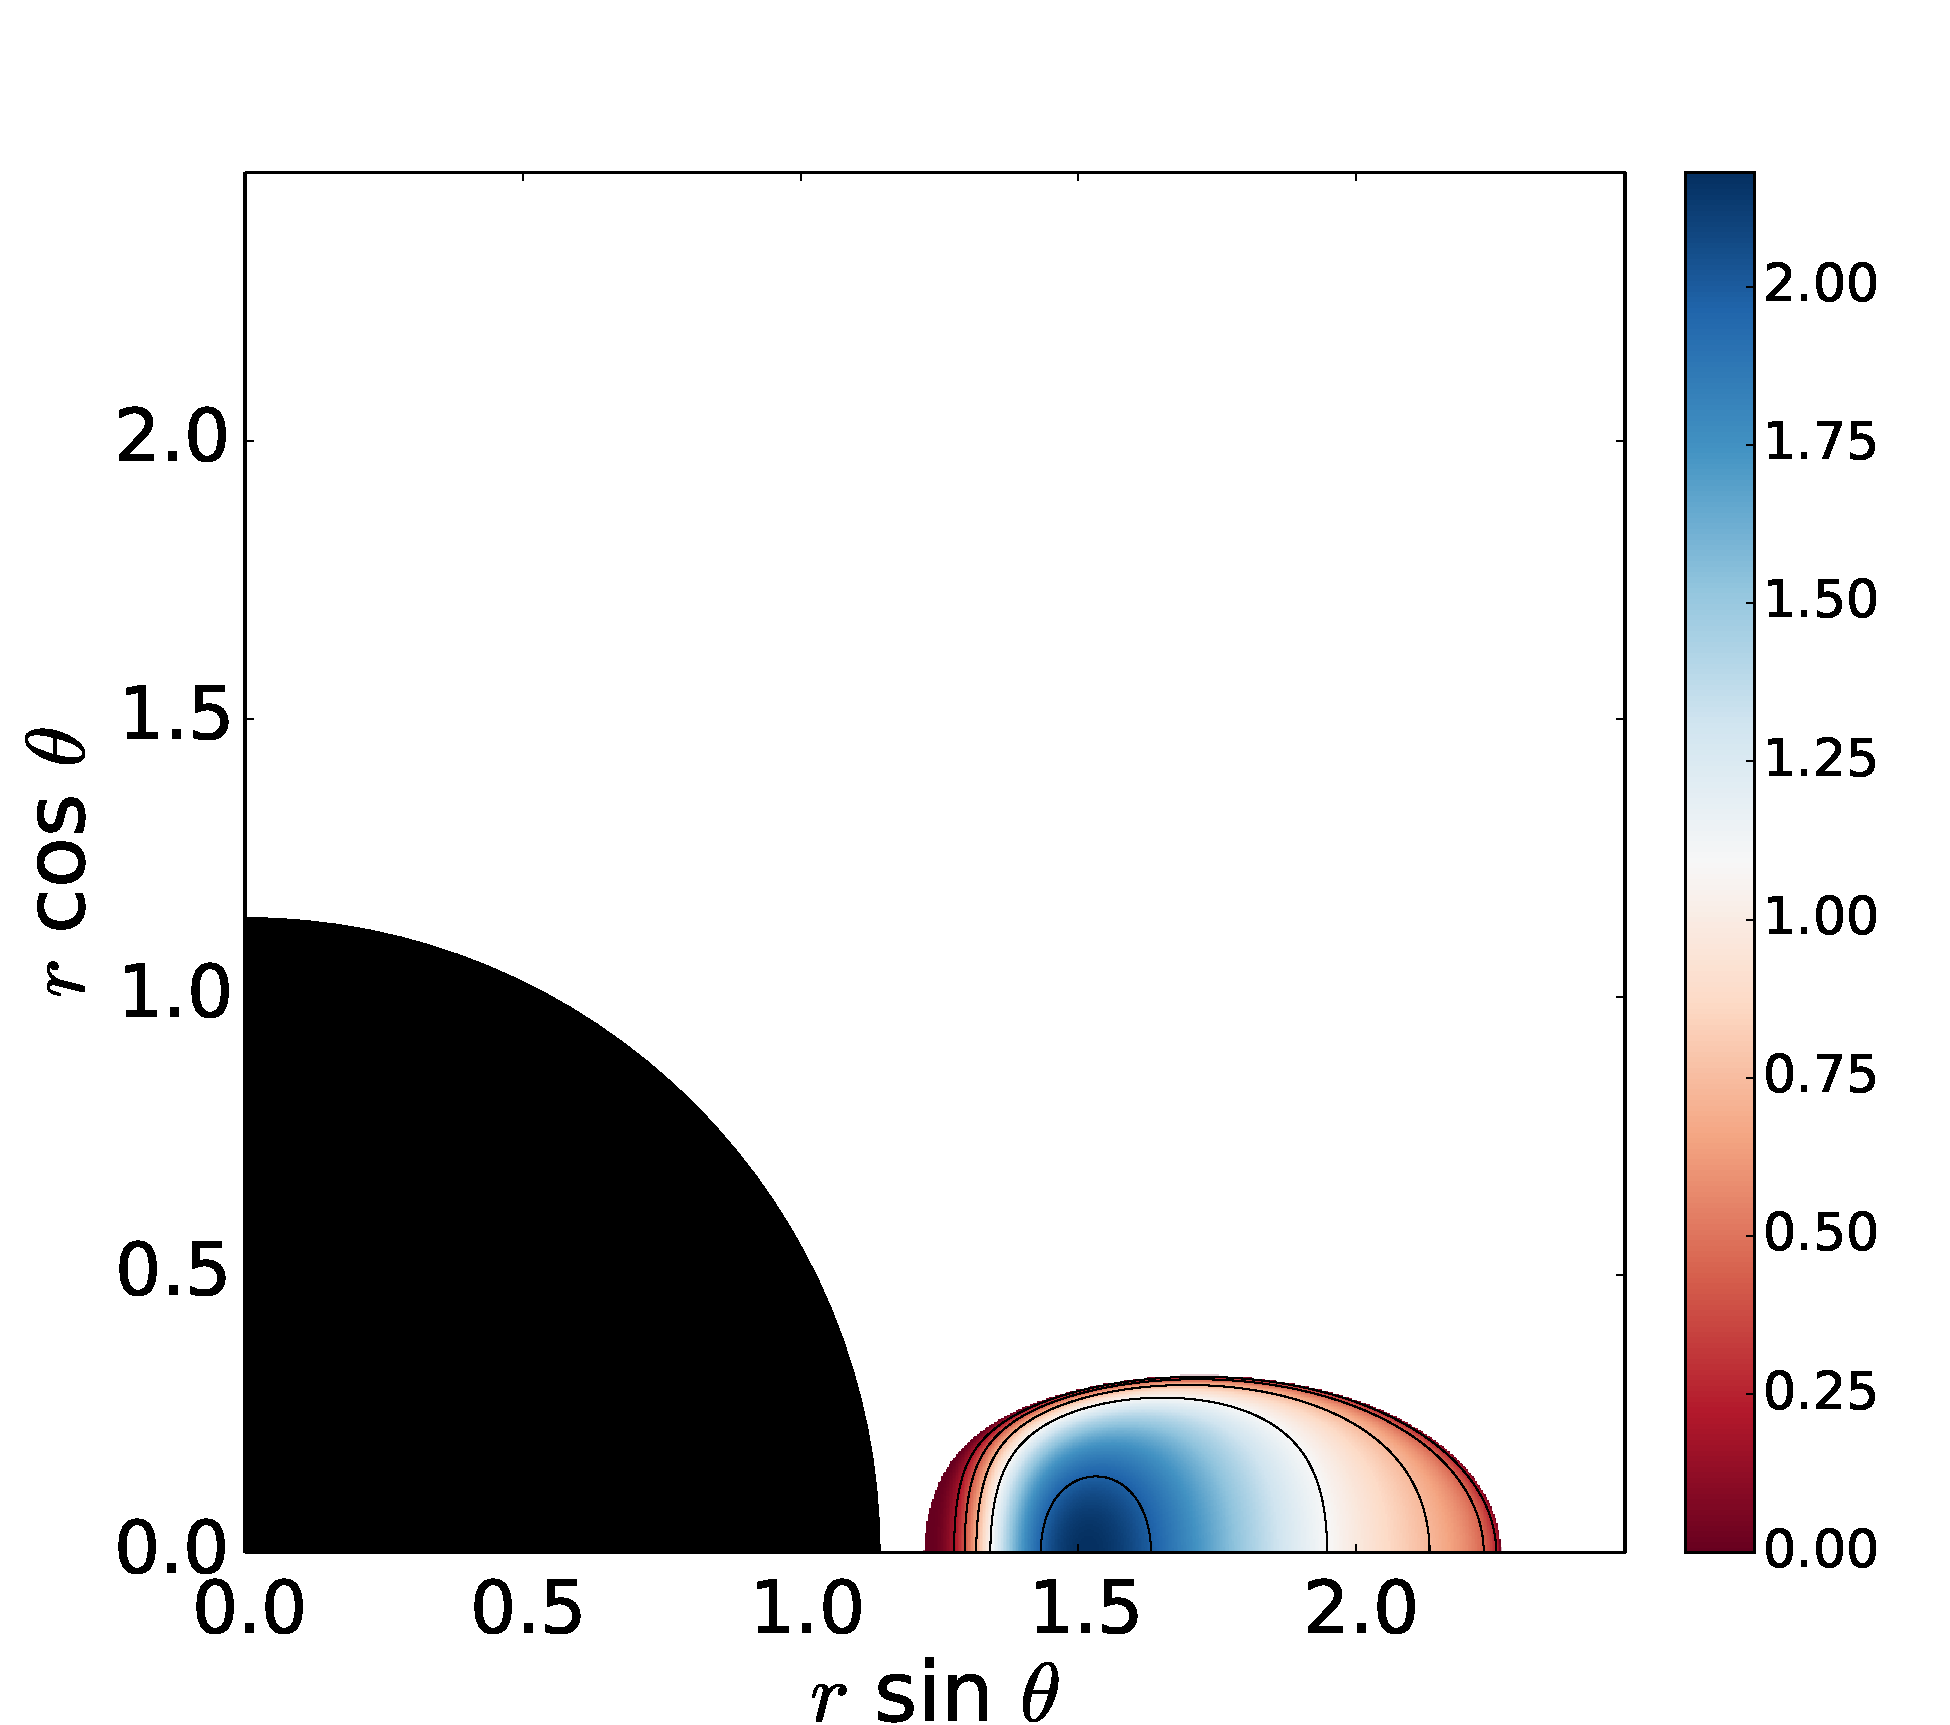
\includegraphics[scale=0.16]{figures/fig2_4_3.pdf}
\\
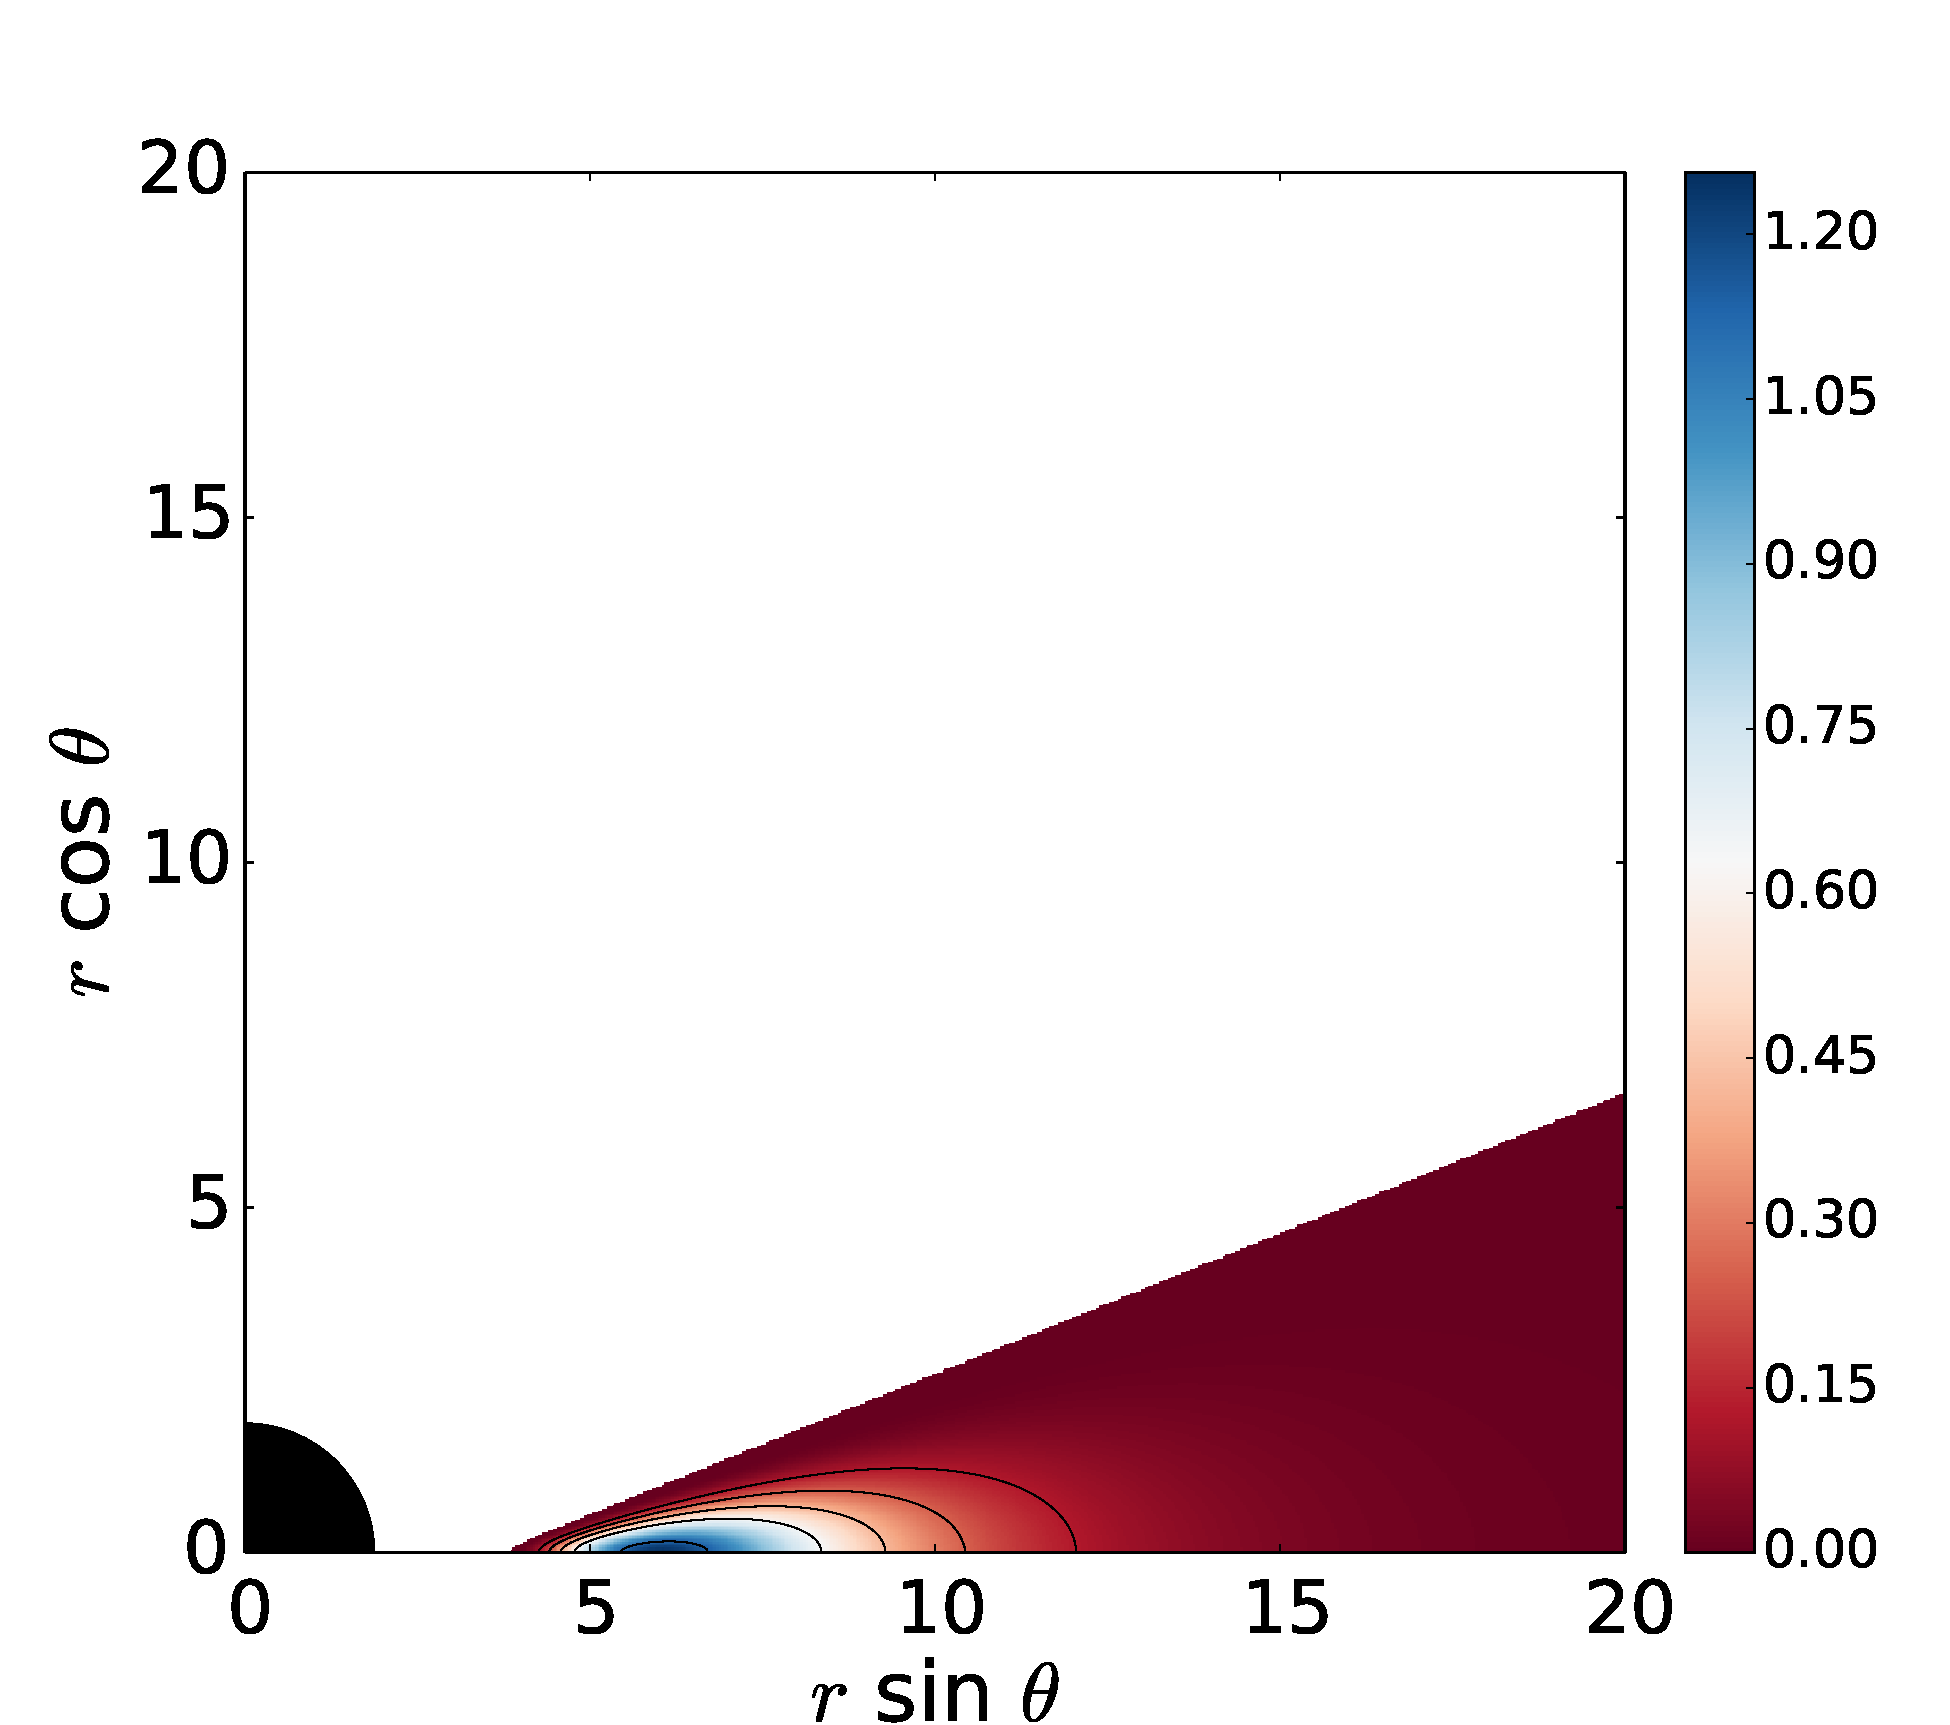
\includegraphics[scale=0.16]{figures/fig2_5_1.pdf}
\hspace{-0.3cm}
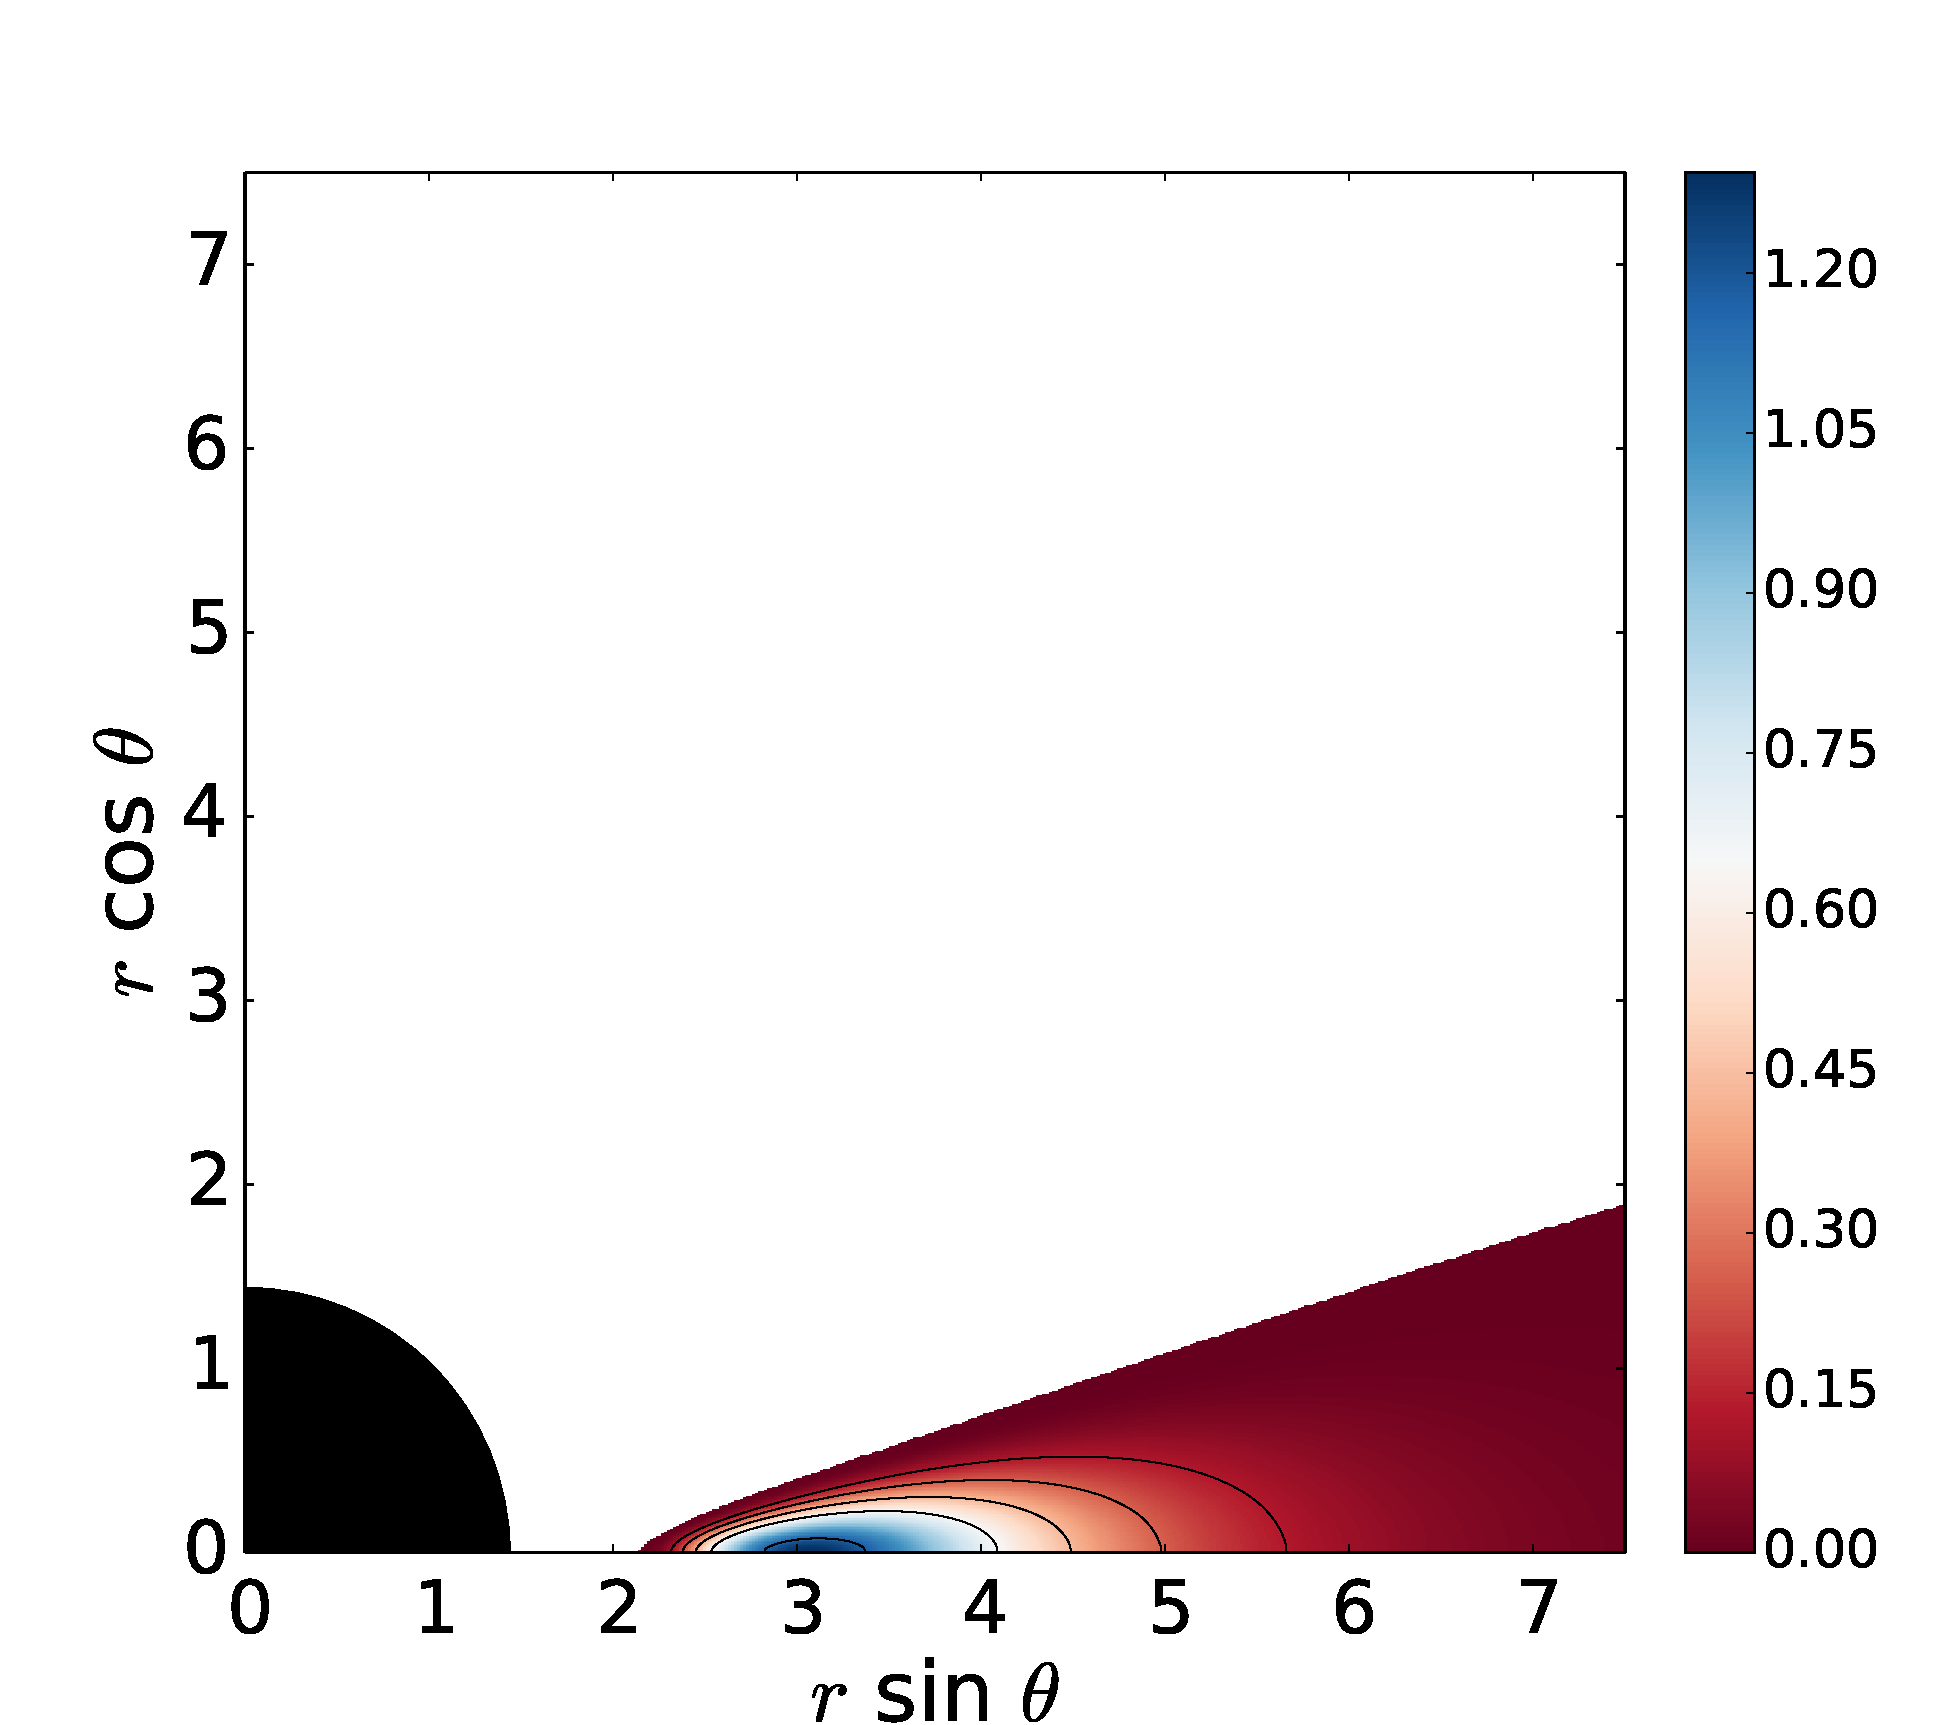
\includegraphics[scale=0.16]{figures/fig2_5_2.pdf}
\hspace{-0.2cm}
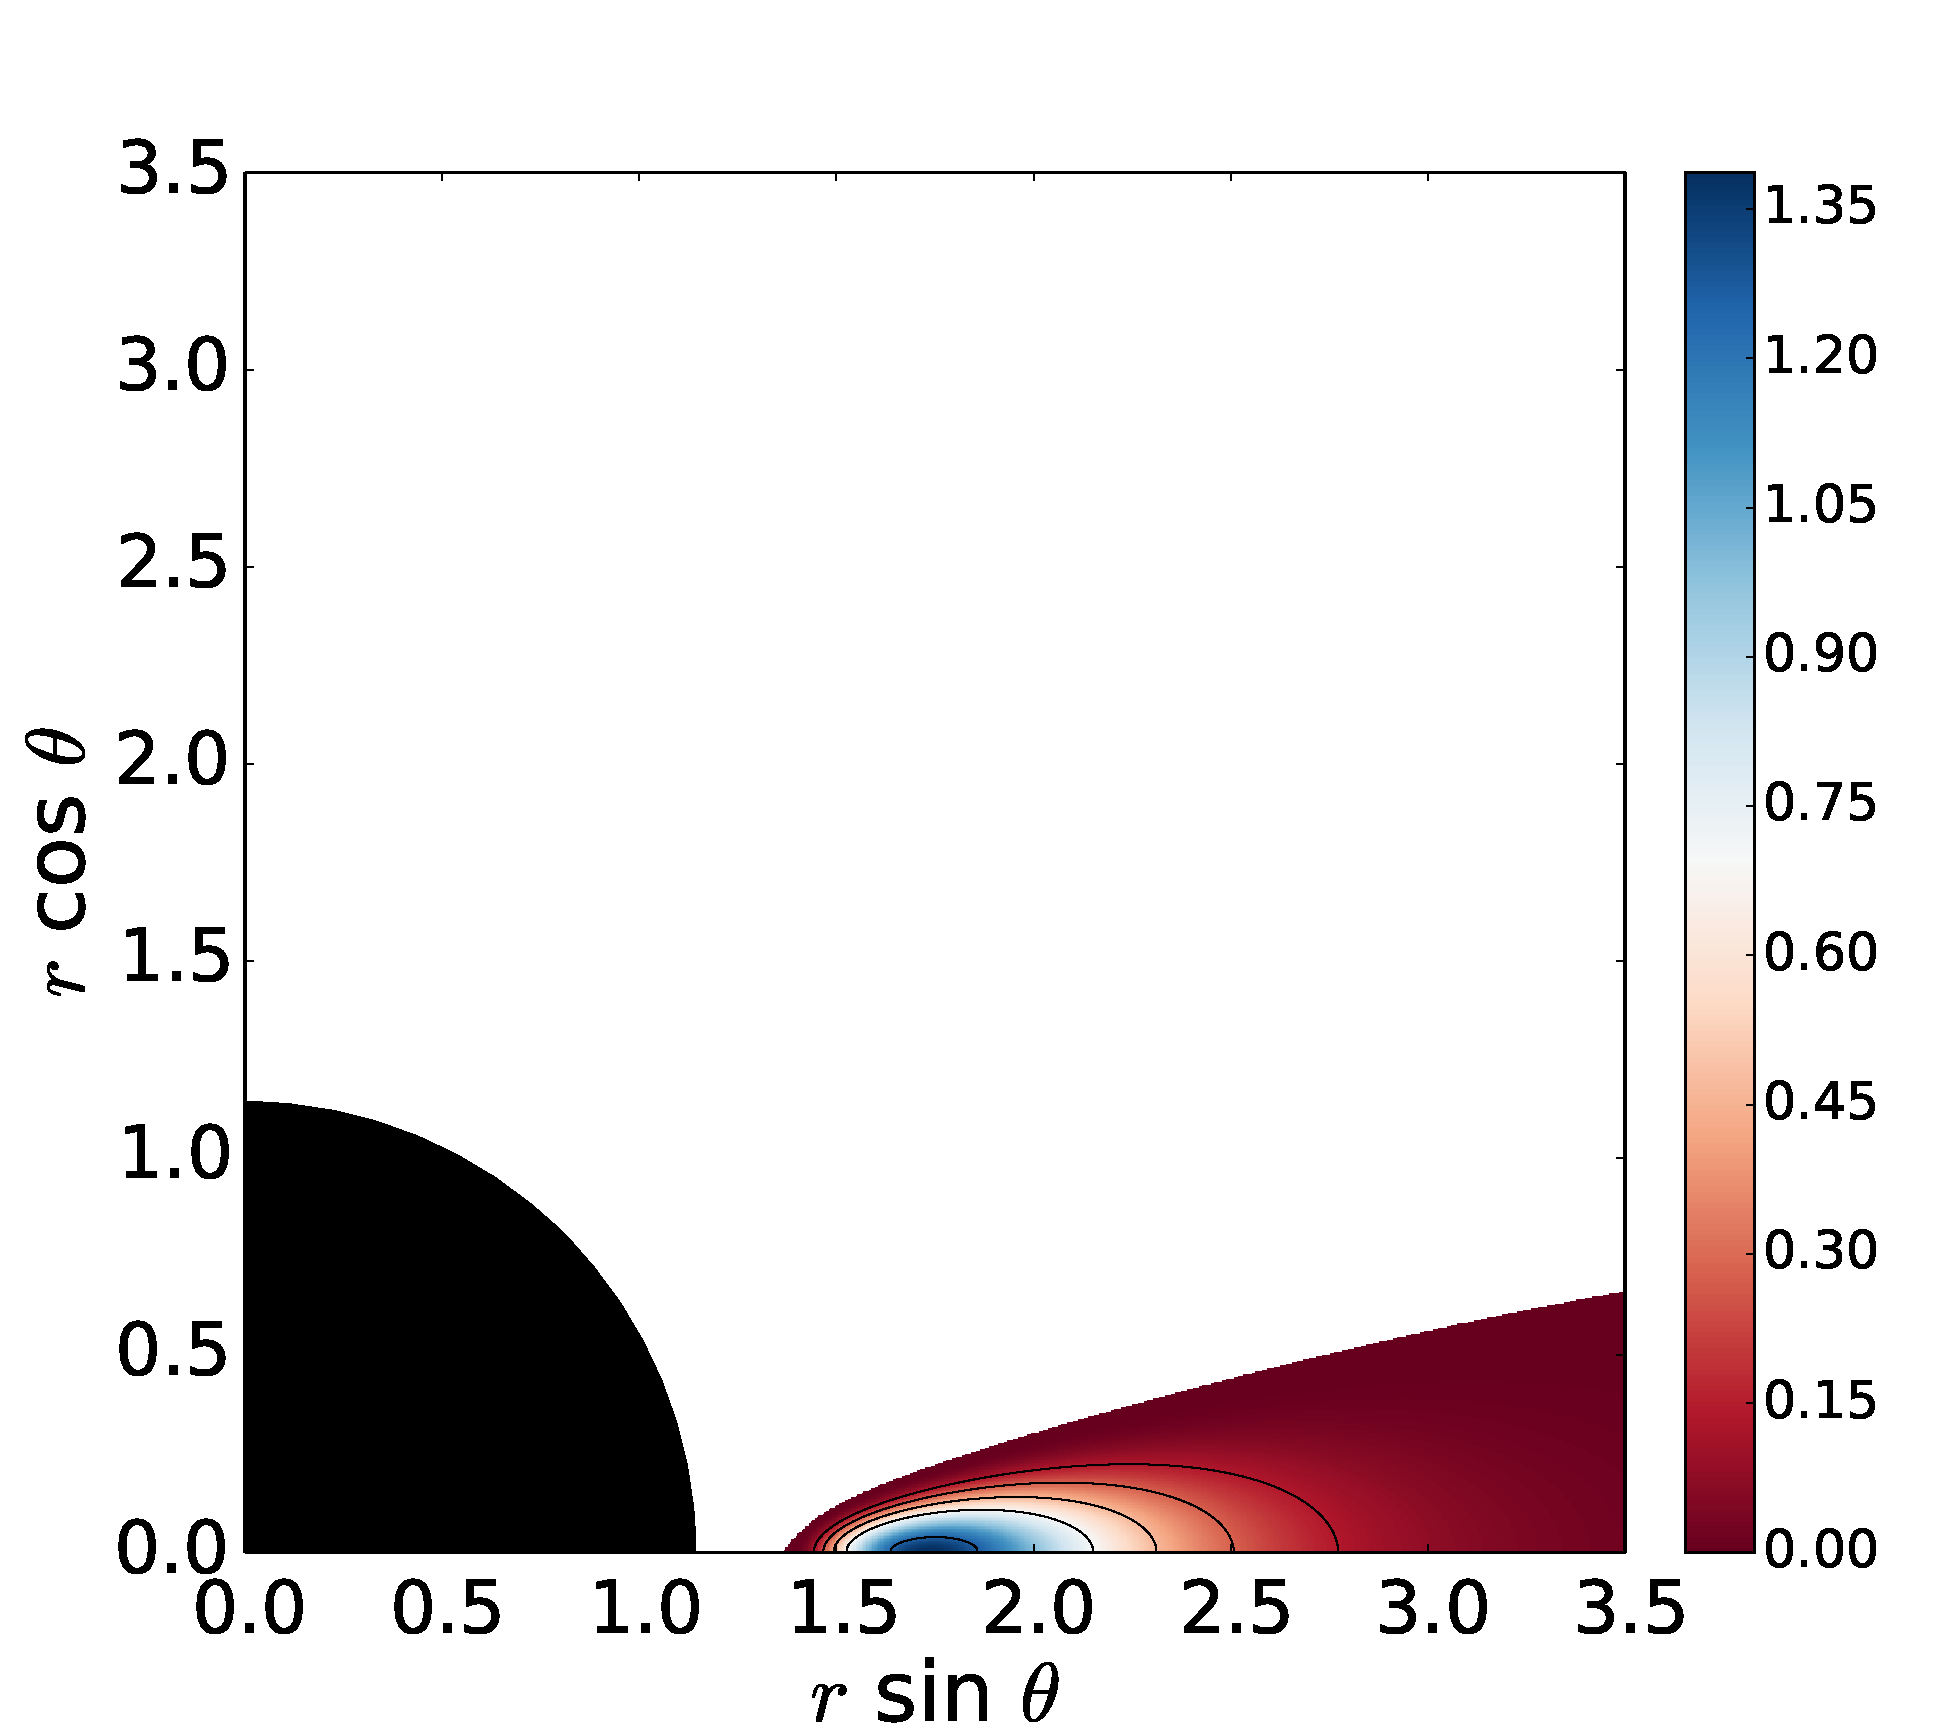
\includegraphics[scale=0.16]{figures/fig2_5_3.pdf}
\caption{Isodensity distributions for a representative sample of our models. From left to right the columns correspond to increasing values of the black hole spin: $a=0.5$, 0.9 and 0.99. From top to bottom the rows correspond to the following parameter combinations: a) $\gamma=\beta=0$; b) $\gamma=\beta=0.5$; c) $\gamma=\beta=0.9$; d) $\gamma=0.9$, $\beta=0$; e) $\gamma=0$, $\beta=0.9$. Note that the spatial scale of the plots differs as it has been chosen to facilitate the visualization of the disks.}
\label{models}
\end{figure*}

\begin{figure*}[t]
\centering
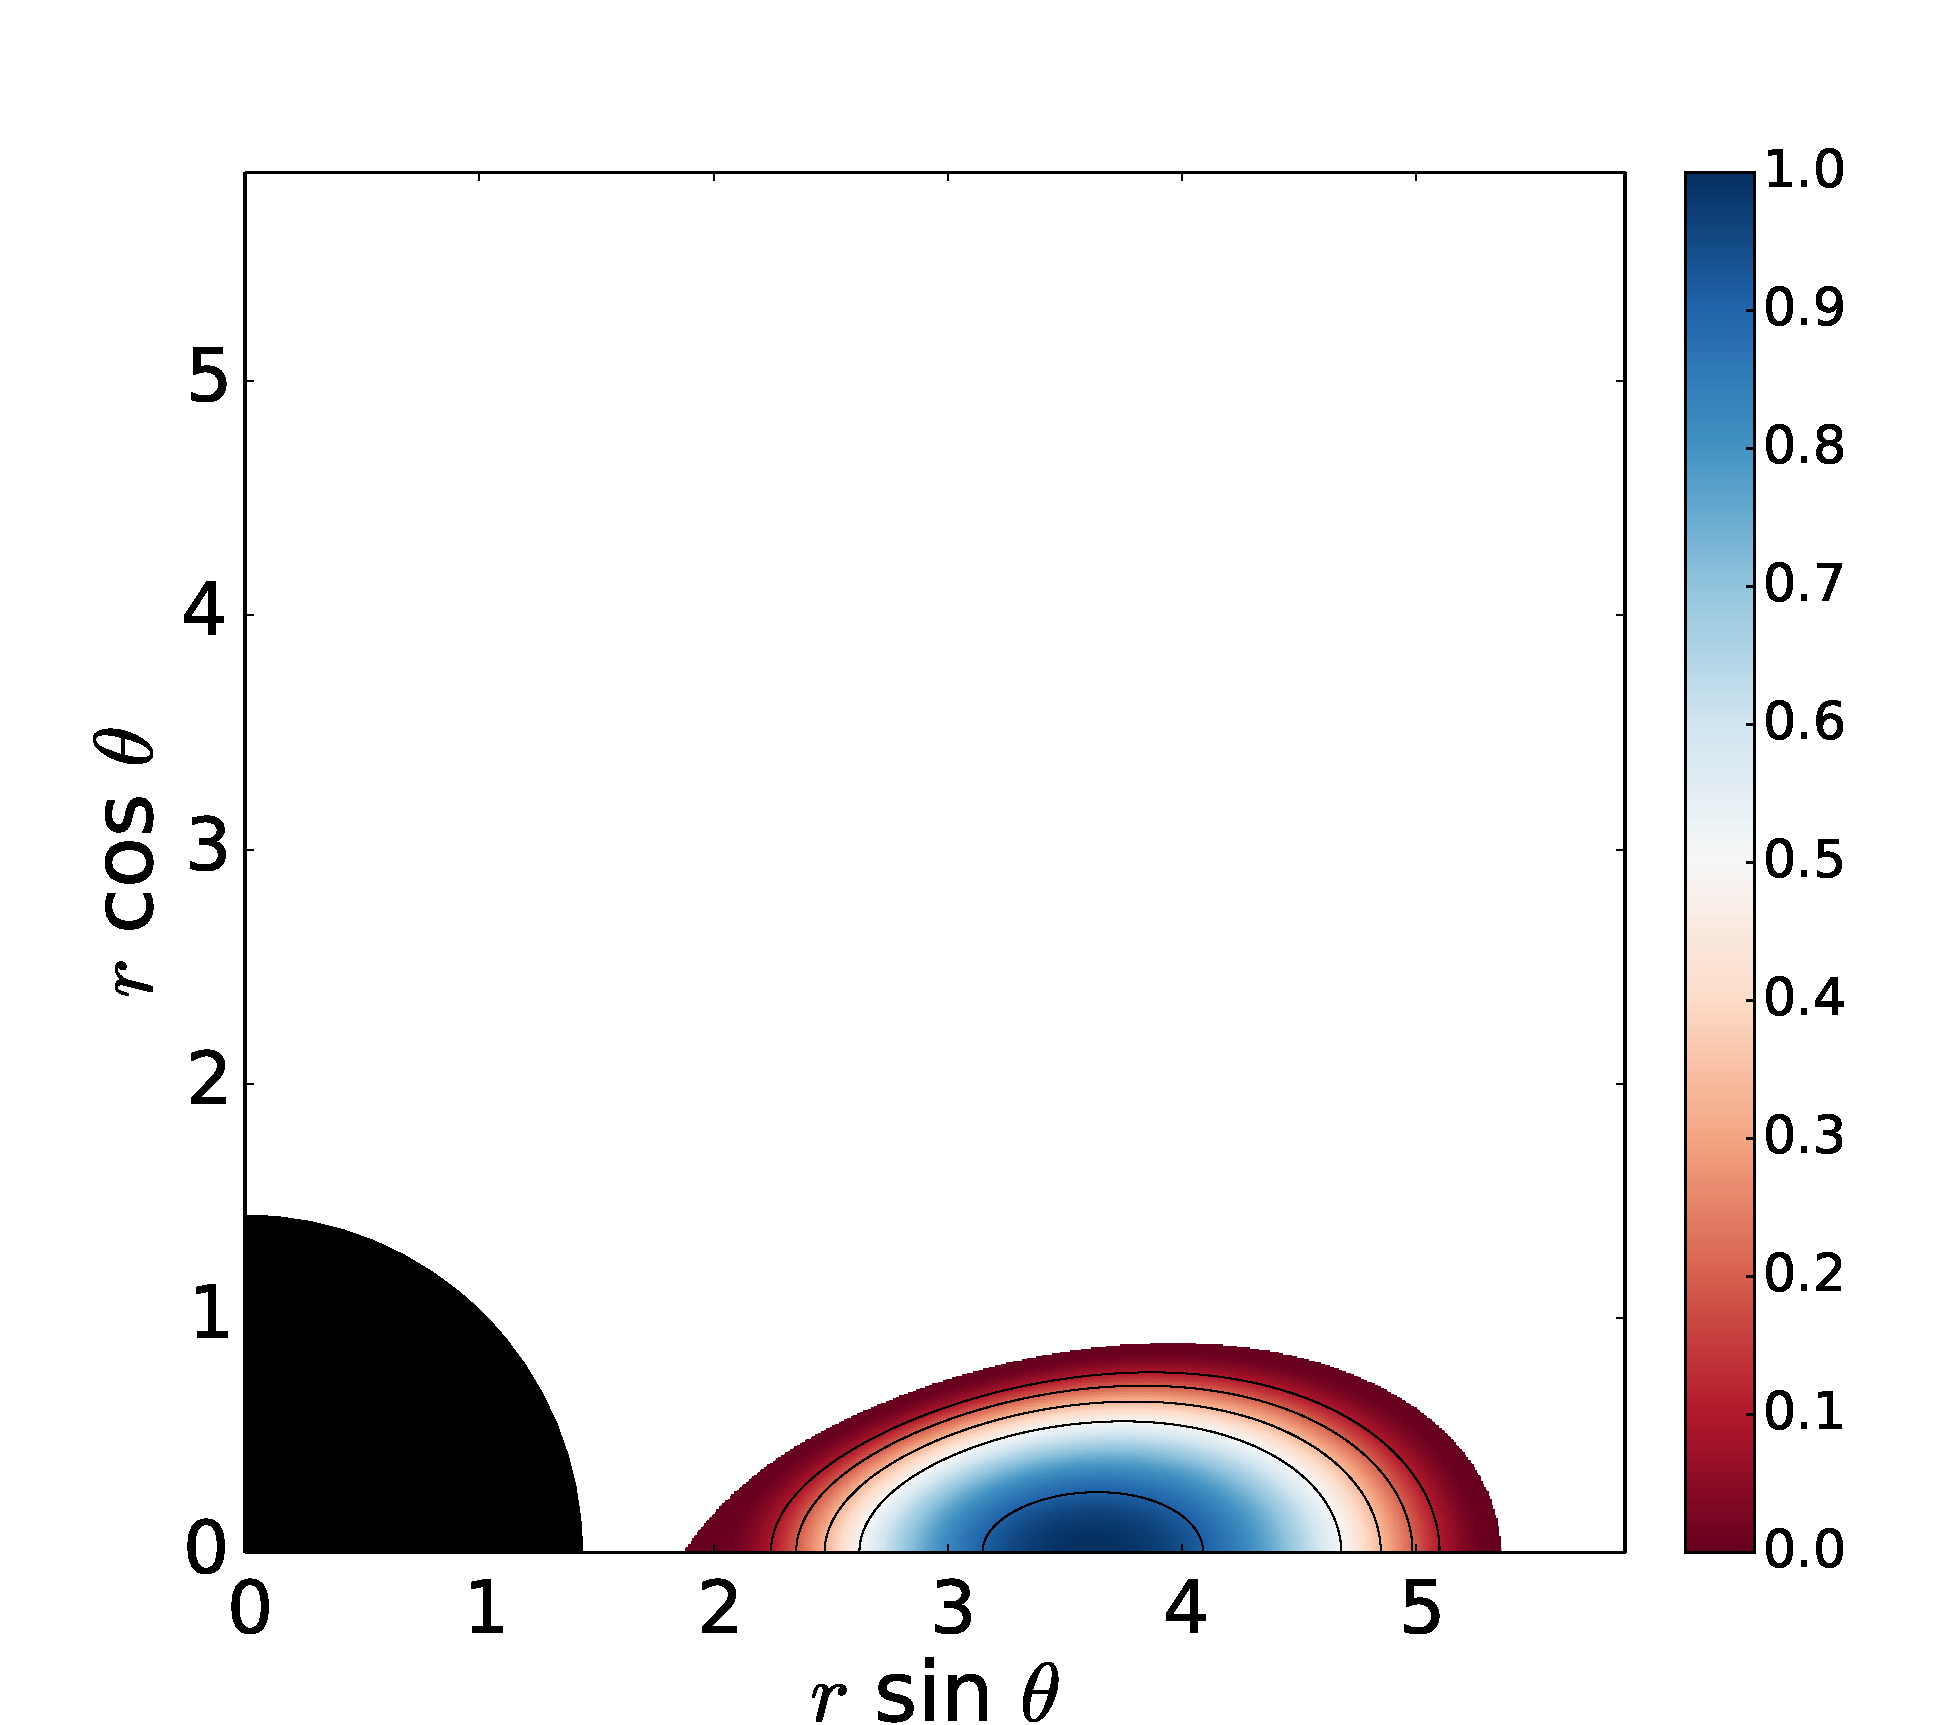
\includegraphics[scale=0.16]{figures/fig3a.pdf}
\hspace{-0.3cm}
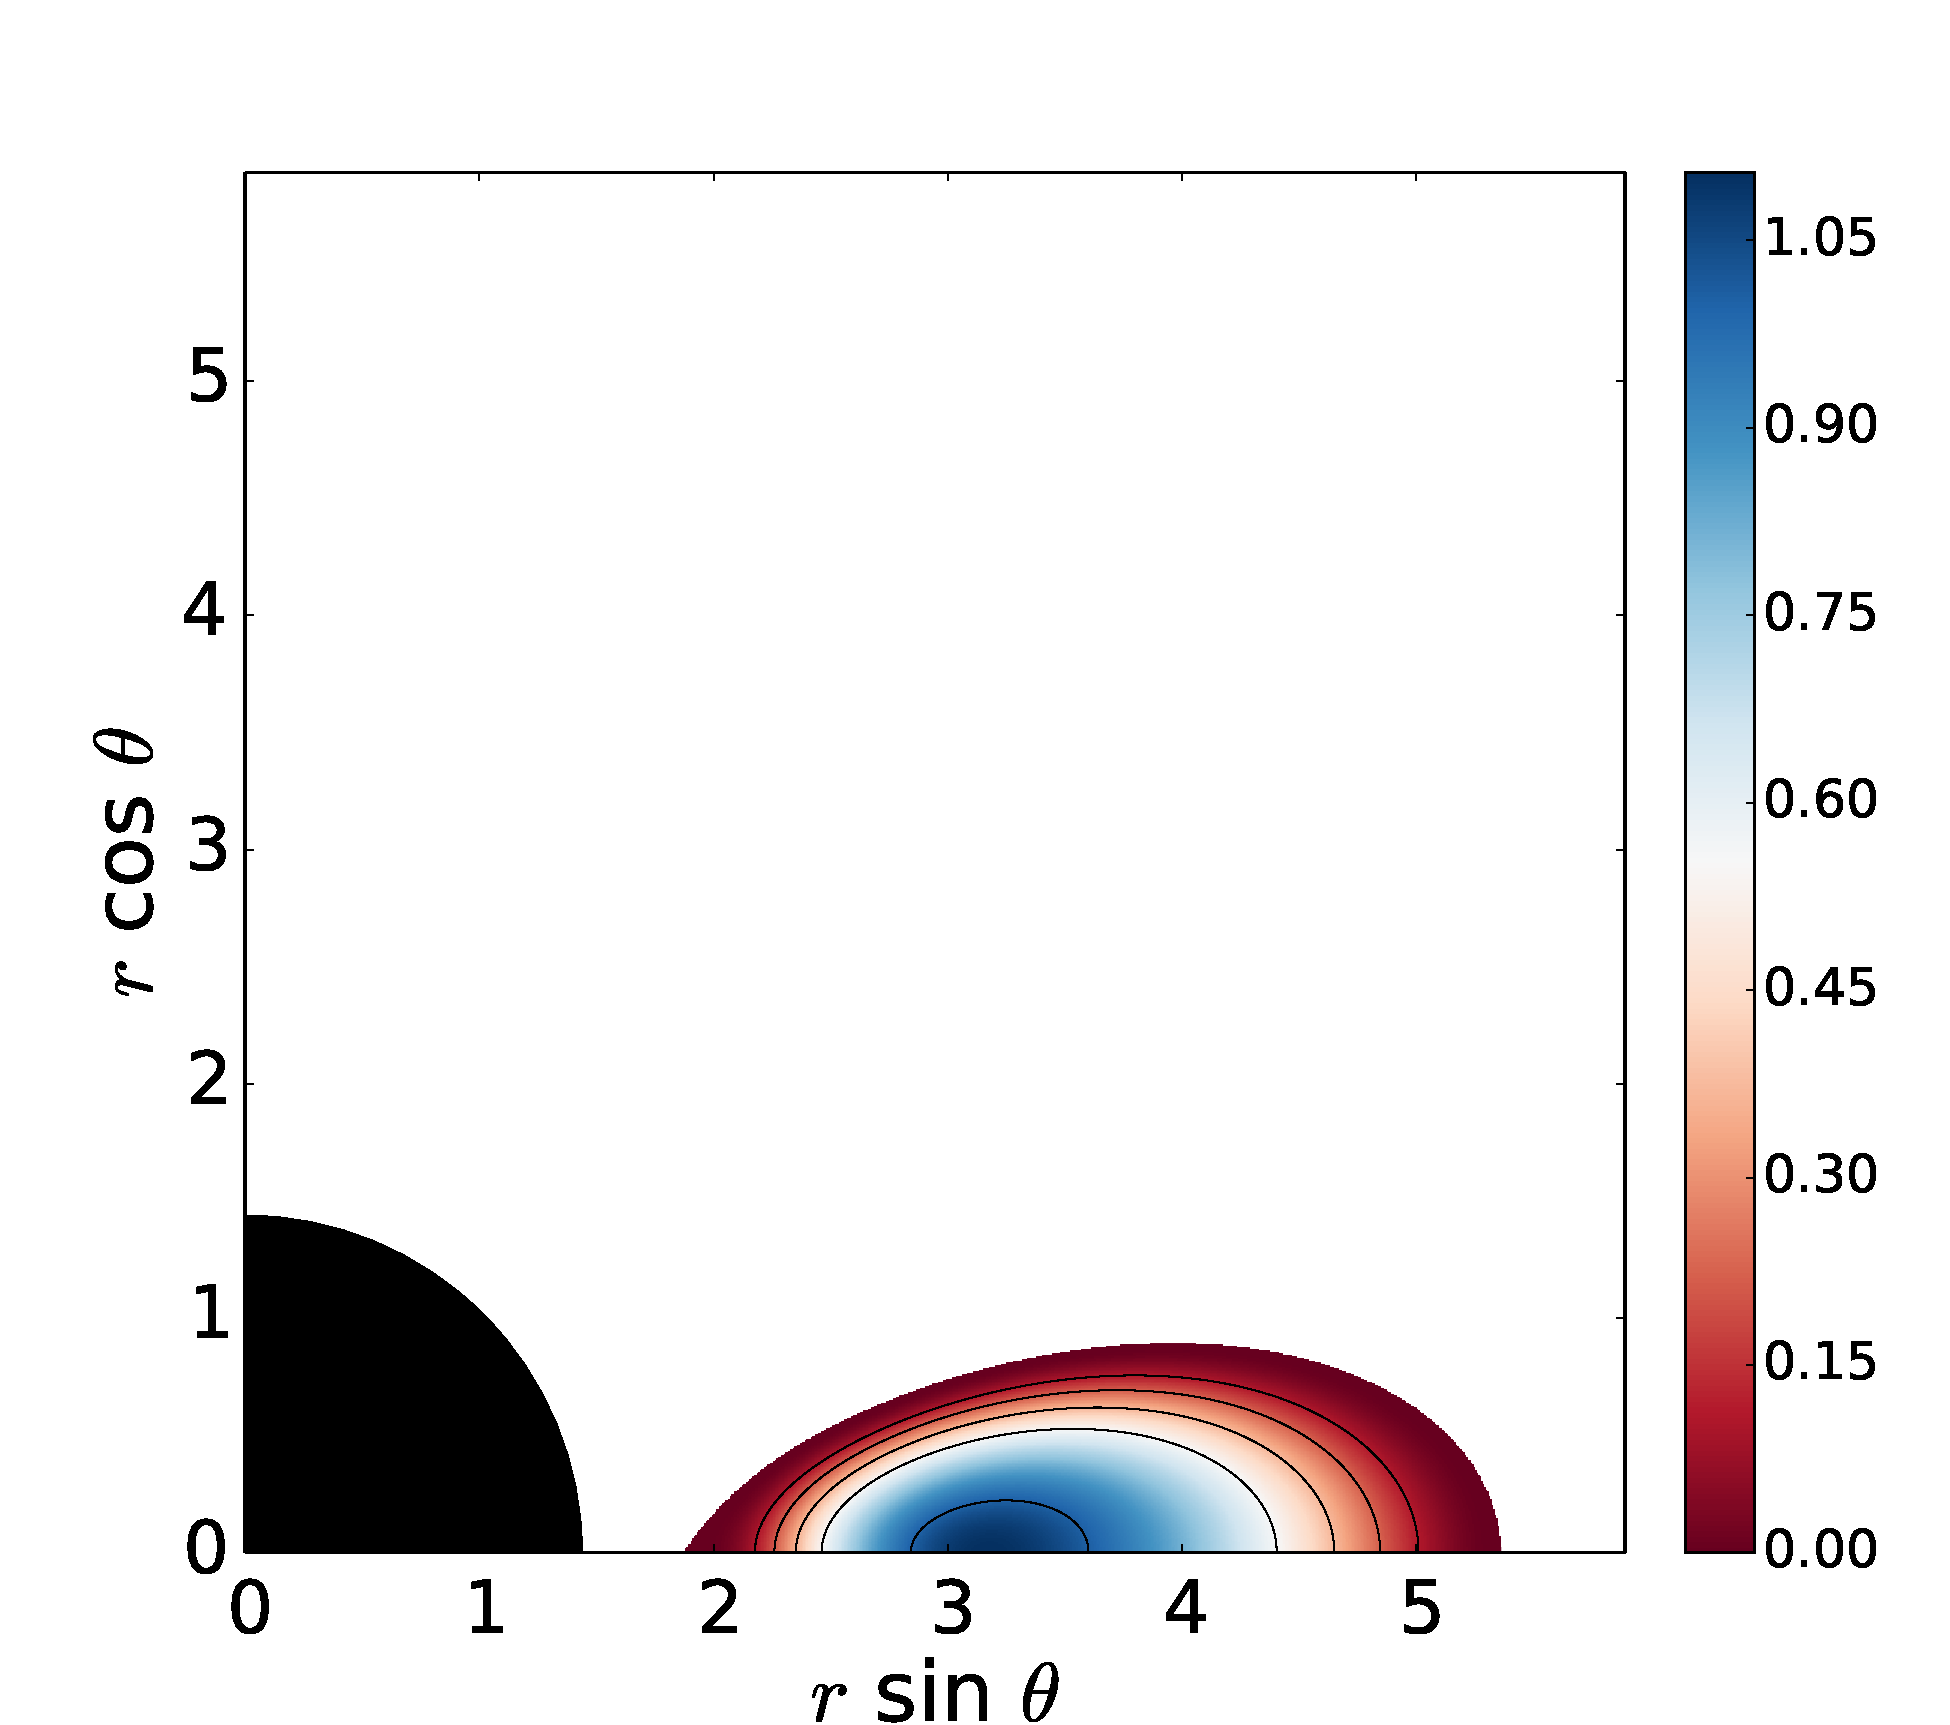
\includegraphics[scale=0.16]{figures/fig3b.pdf}
\hspace{-0.2cm}
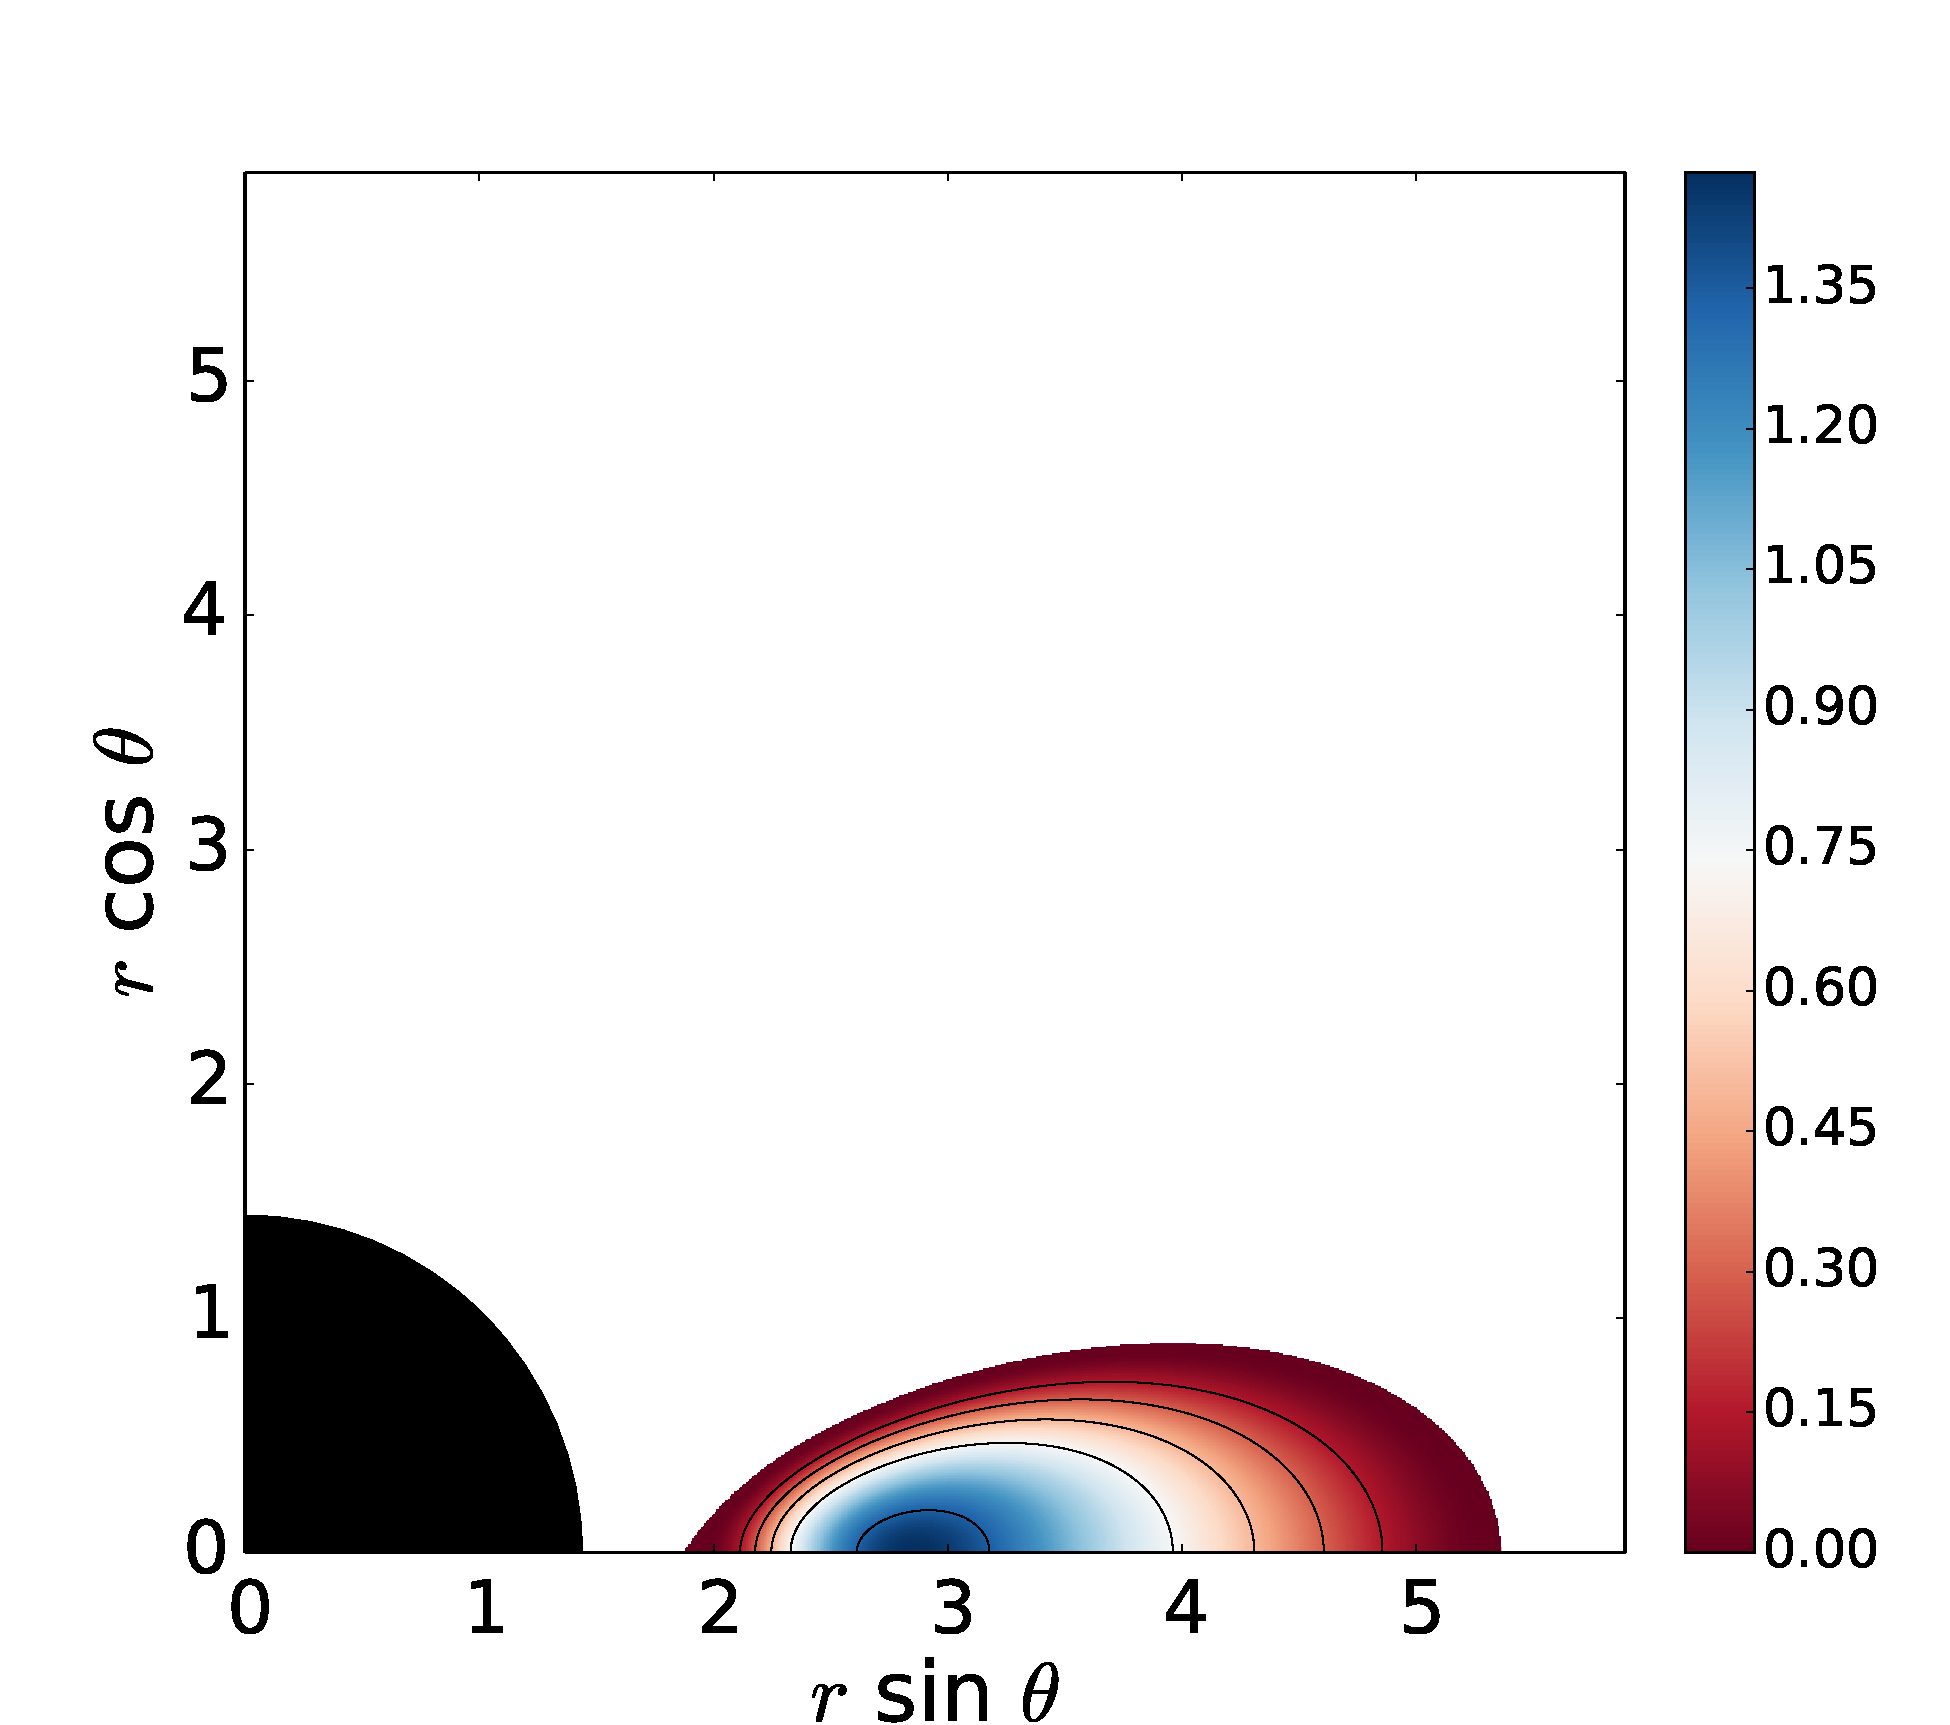
\includegraphics[scale=0.16]{figures/fig3c.pdf}
\caption{Effects of the magnetization in the structure of the disk. From left to right the values are $\beta_{\mathrm{m}_{\mathrm{c}}}
=10^3$, 1, and $10^{-3}$.}
\label{magnetization}%
\end{figure*}

We start by assessing our procedure by first building a disk that can be directly compared with one of the two models in~\citet{Komissarov:2006}. This is shown in Figure~\ref{komissarov}, which corresponds to the same constant specific angular momentum model A presented by~\citet{Komissarov:2006}. The parameters of this model are $a=0.9$, $\beta_{\mathrm{m}_{\mathrm{c}}}=0.1$, and $l=2.8$.
The visual comparison shows that our approach can reproduce those previous results with good agreement. The density distribution in the $(r\sin\theta,r\cos\theta)$ plane shown in the left panel of Fig.~\ref{komissarov} is remarkably similar to that shown in the left panel of Fig.~2 in~\citet{Komissarov:2006}. Not only the morphology of both models is nearly identical but also the range of variation of the density and the location of the disk center agree well in both cases. This can be most clearly seen in the middle and right panels of Fig.~\ref{komissarov} which show, repectively, the angular profile at $r_{\rm c}$ and the radial profile at $\theta=\pi/2$. These two figures can be directly compared with Fig.~3 of~\citet{Komissarov:2006}. It is relevant to mention that very small changes in the inner radius $r_{\mathrm{in}}$ have a significant effect on the maximum value of the density, that explains the small differences between our figures and the ones presented in~\citet{Komissarov:2006}.

\begin{figure}[t]
\centering
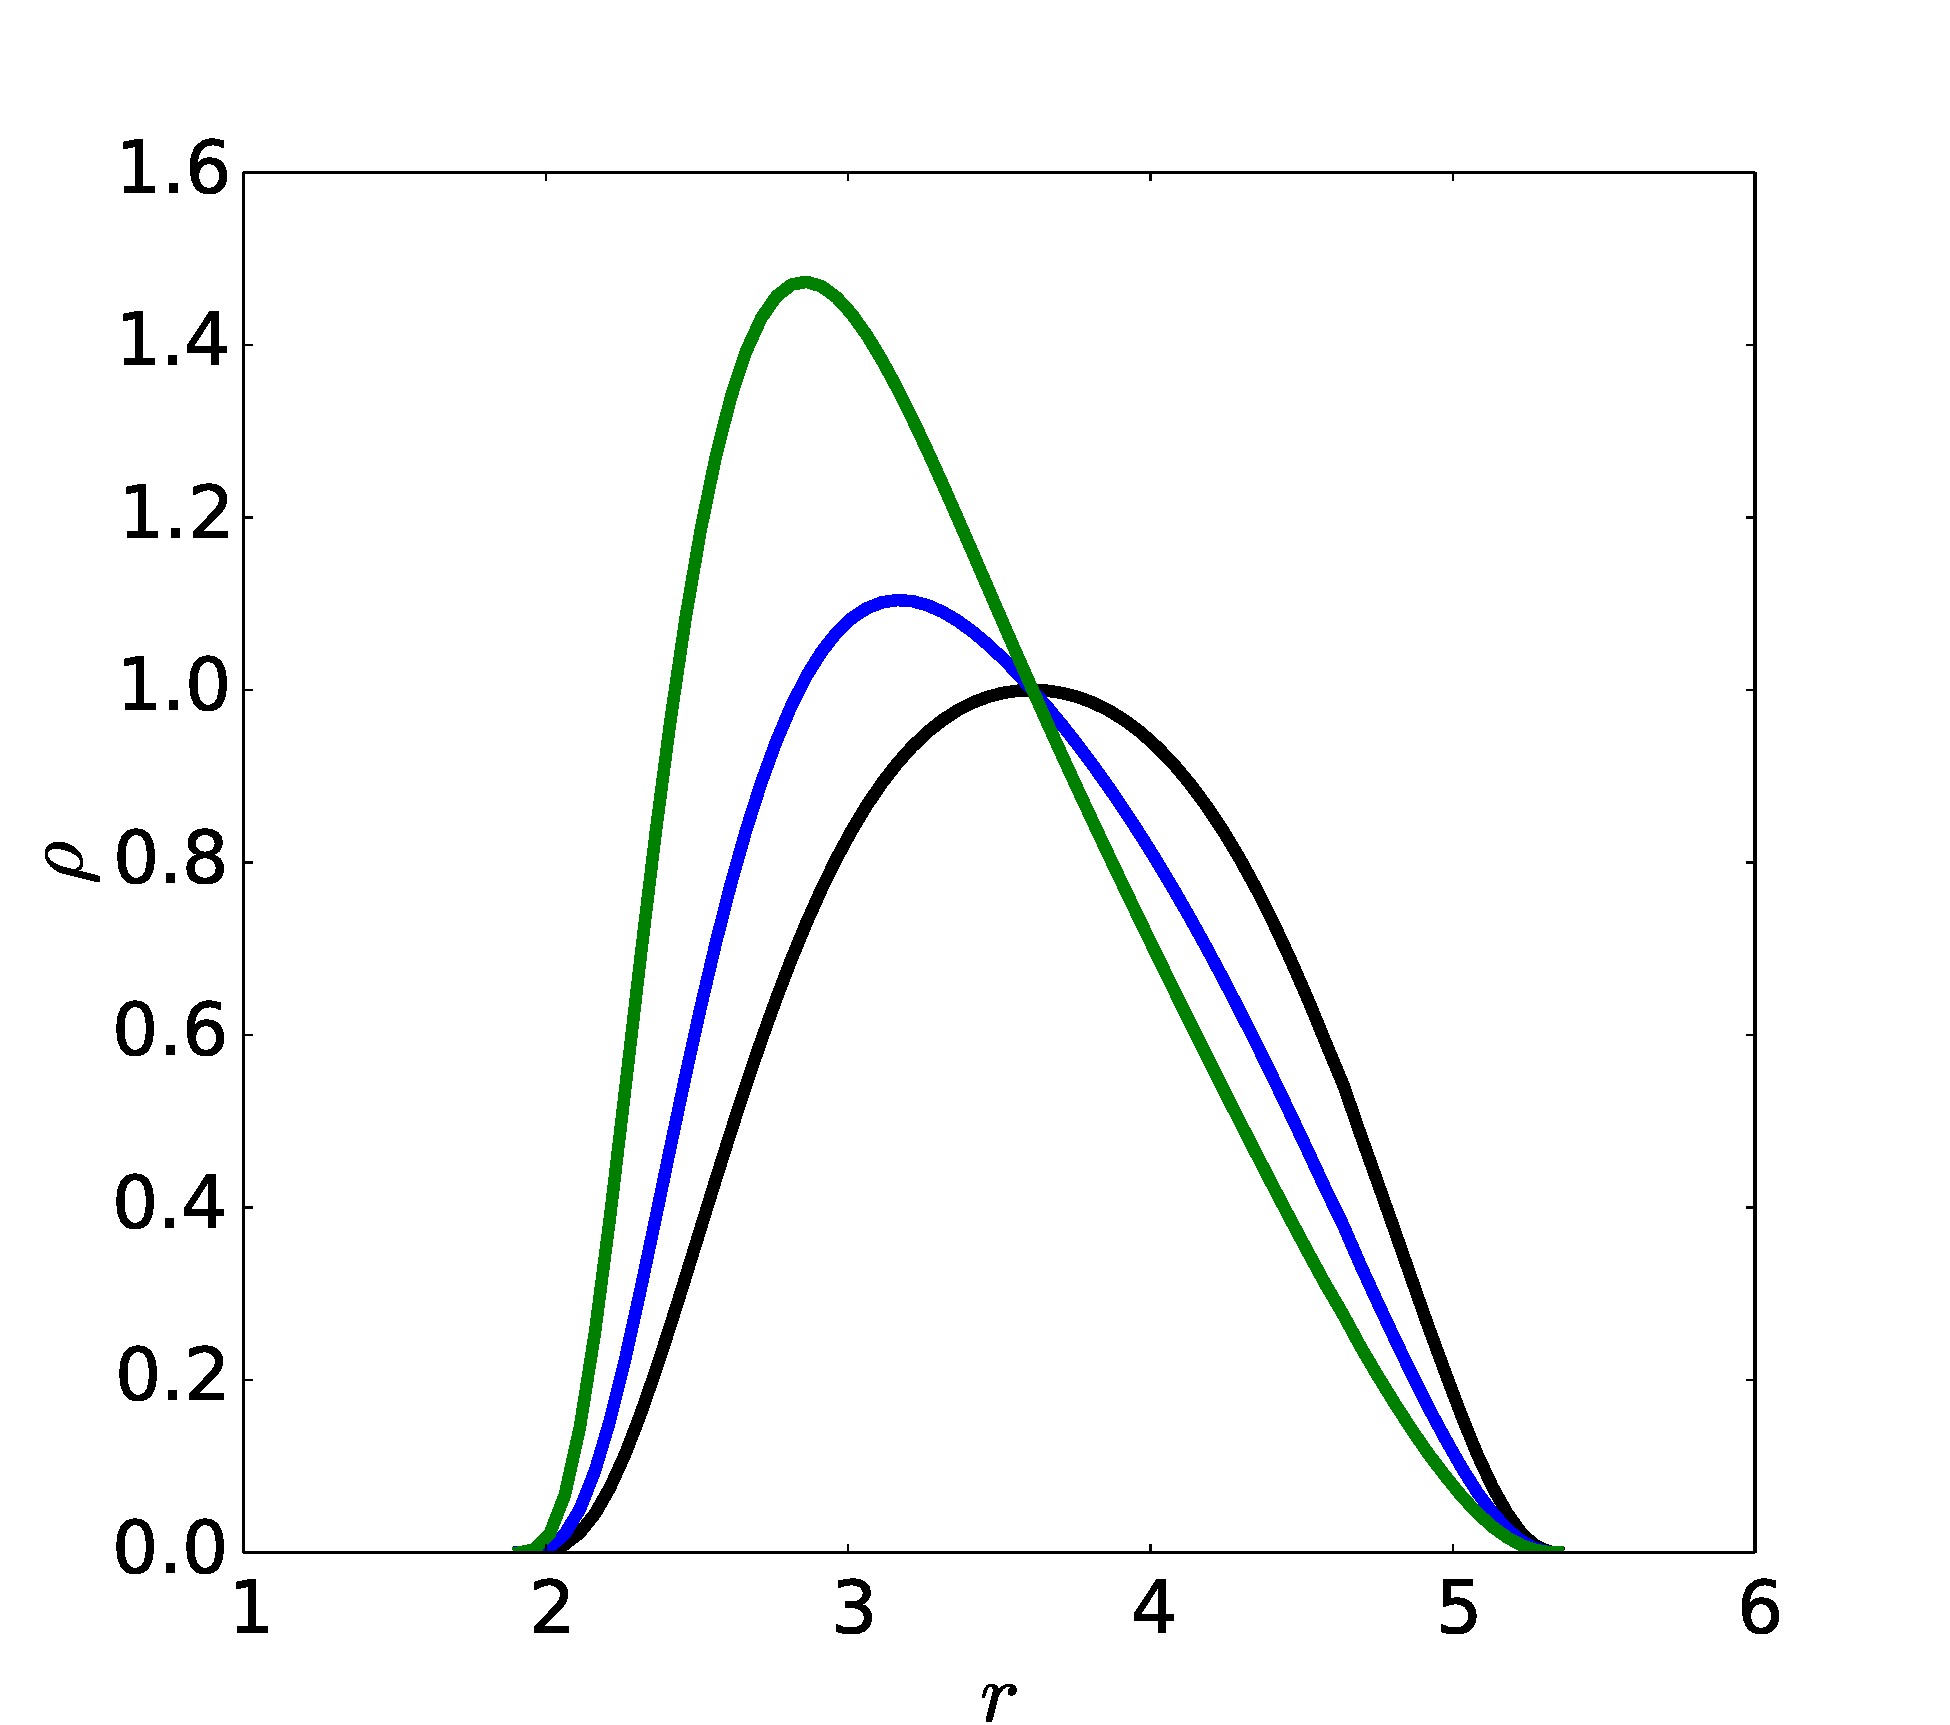
\includegraphics[scale=0.2]{figures/fig4.pdf}
\caption{Radial profiles of the density in the equatorial plane for $\beta=10^3$ (black curve), 1 (blue curve), and $10^{-3}$ (green curve). }
\label{magnetization-profile}
 \end{figure}
 
\begin{figure}[t]
\centering
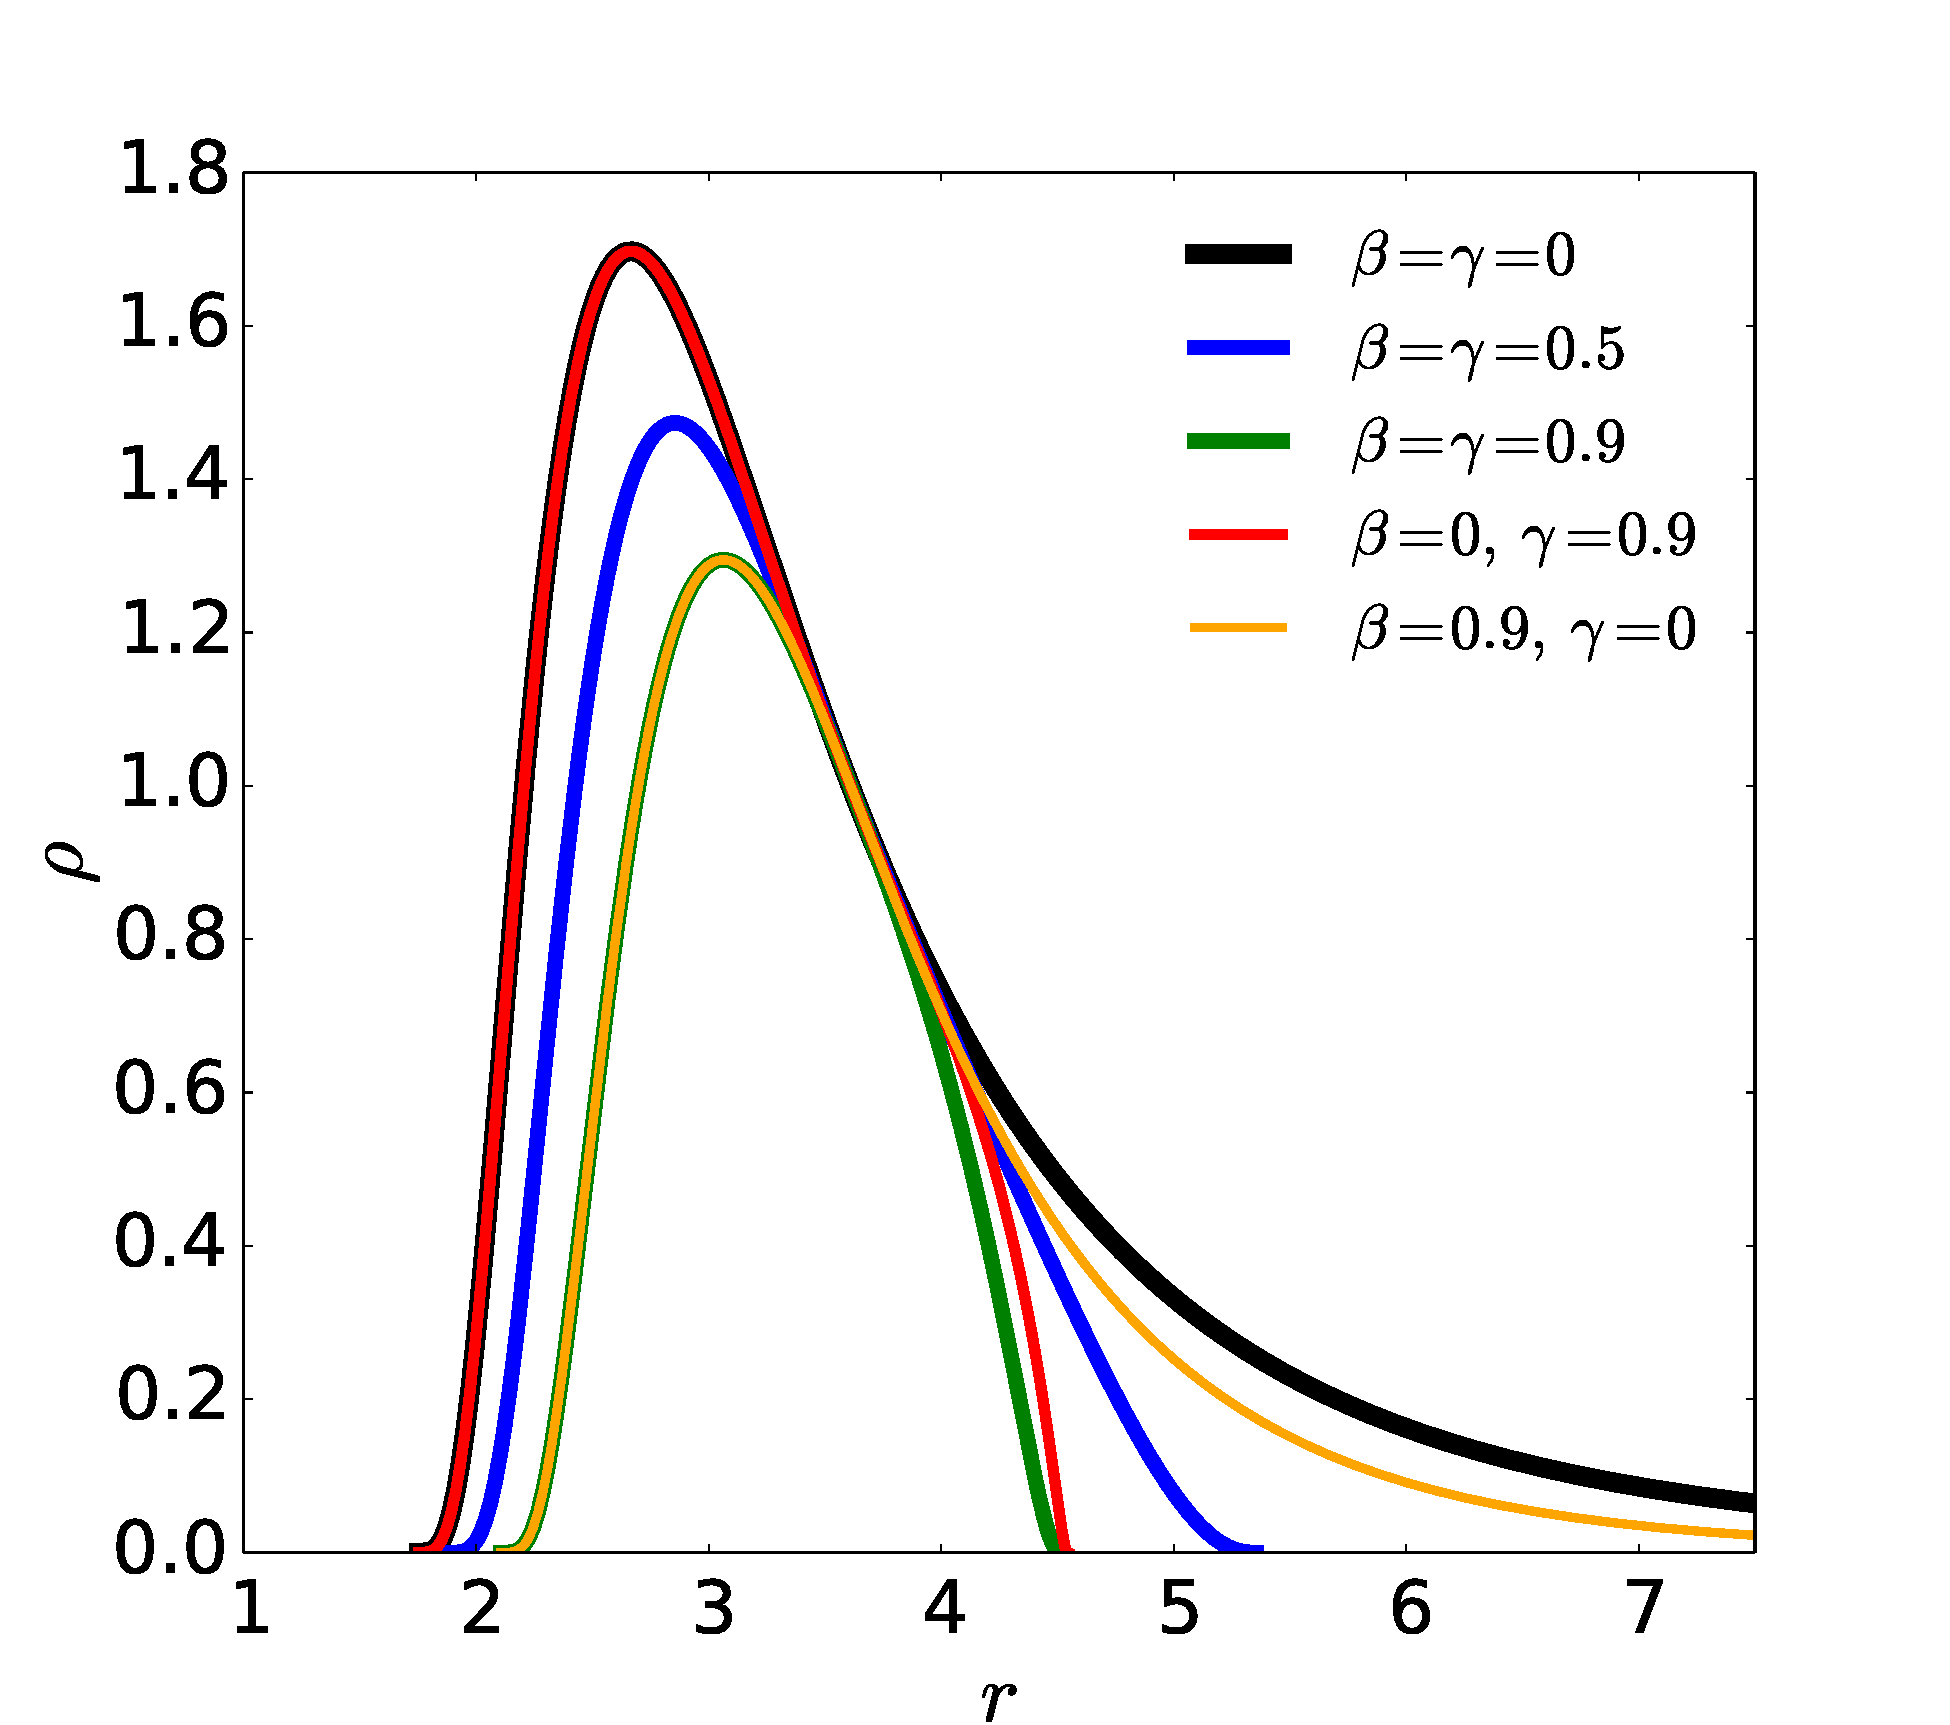
\includegraphics[scale=0.2]{figures/fig5.pdf}
\caption{Radial profiles at the equatorial plane for models with $a=0.9$, $\beta_{\mathrm{m}_{\mathrm{c}}}
=10^{-3}$, and same combination of the $\gamma$ and $\beta$ parameters as in the rows of Fig.~\ref{models} (the specific values are indicated in the legend).}
\label{more-profile}
\end{figure}

\begin{figure*}
\centering
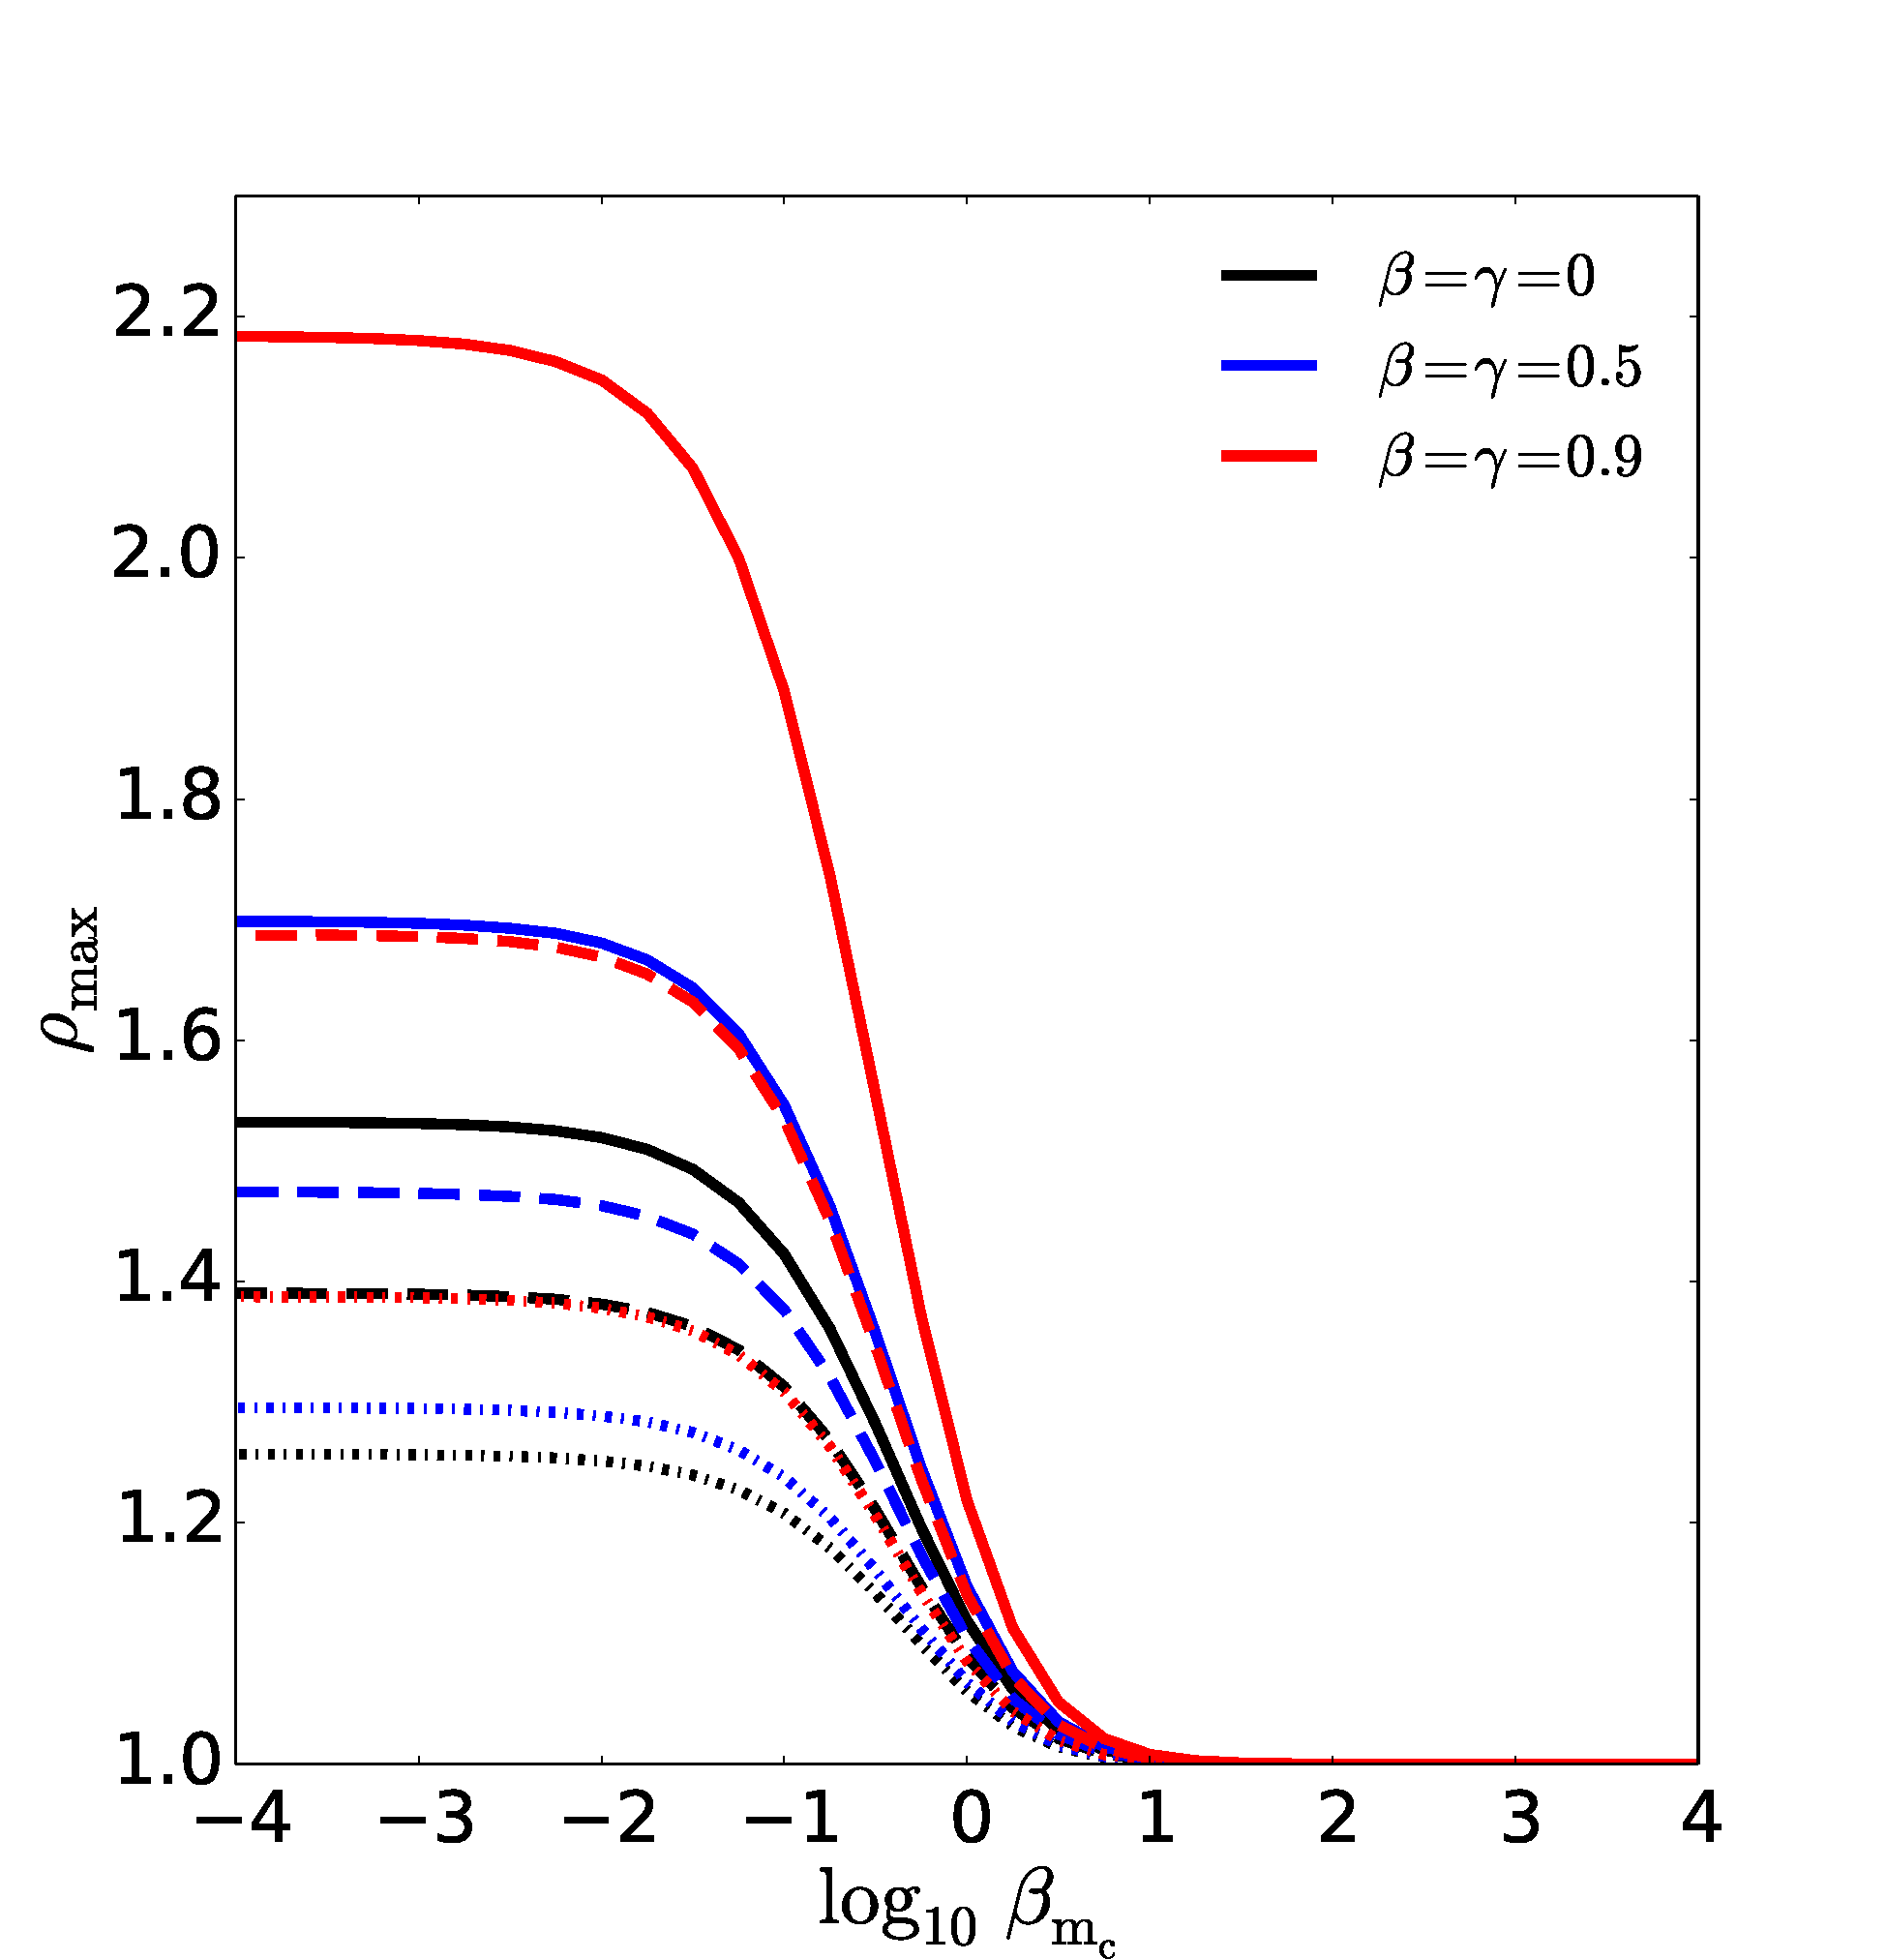
\includegraphics[scale=0.16]{figures/fig6a.pdf}
\hspace{-0.3cm}
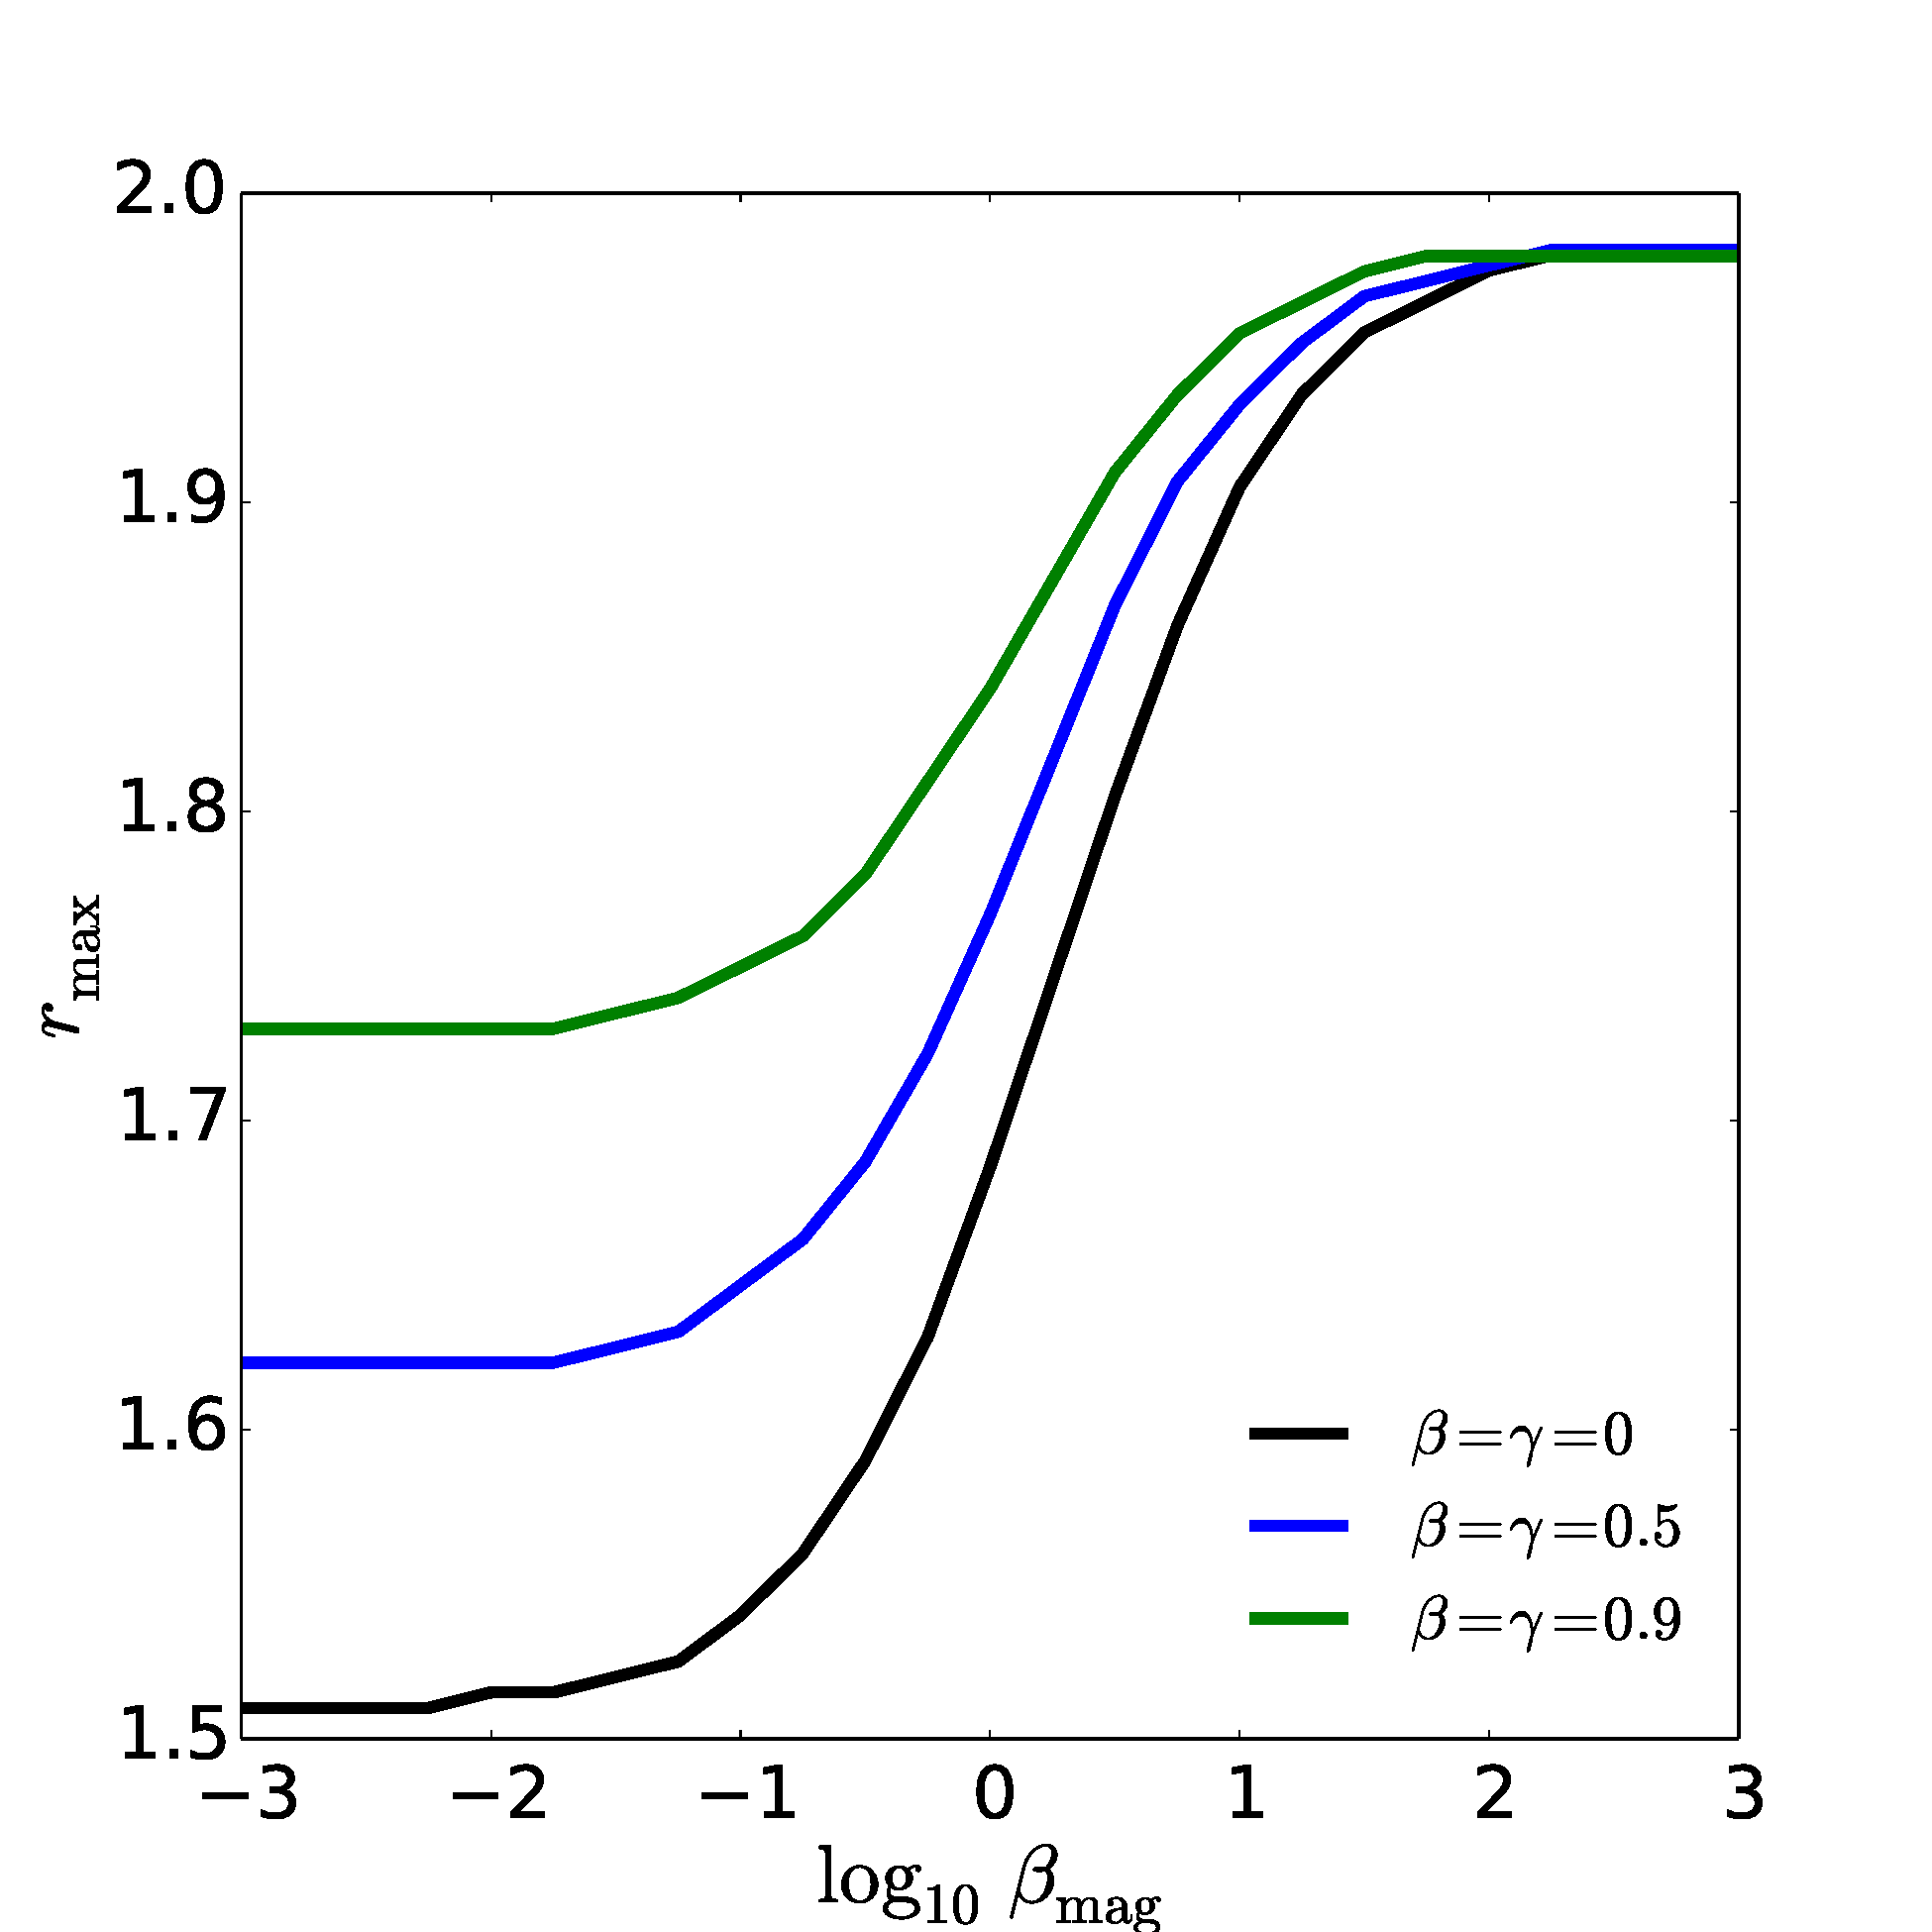
\includegraphics[scale=0.16]{figures/fig6b.pdf}
\hspace{-0.2cm}
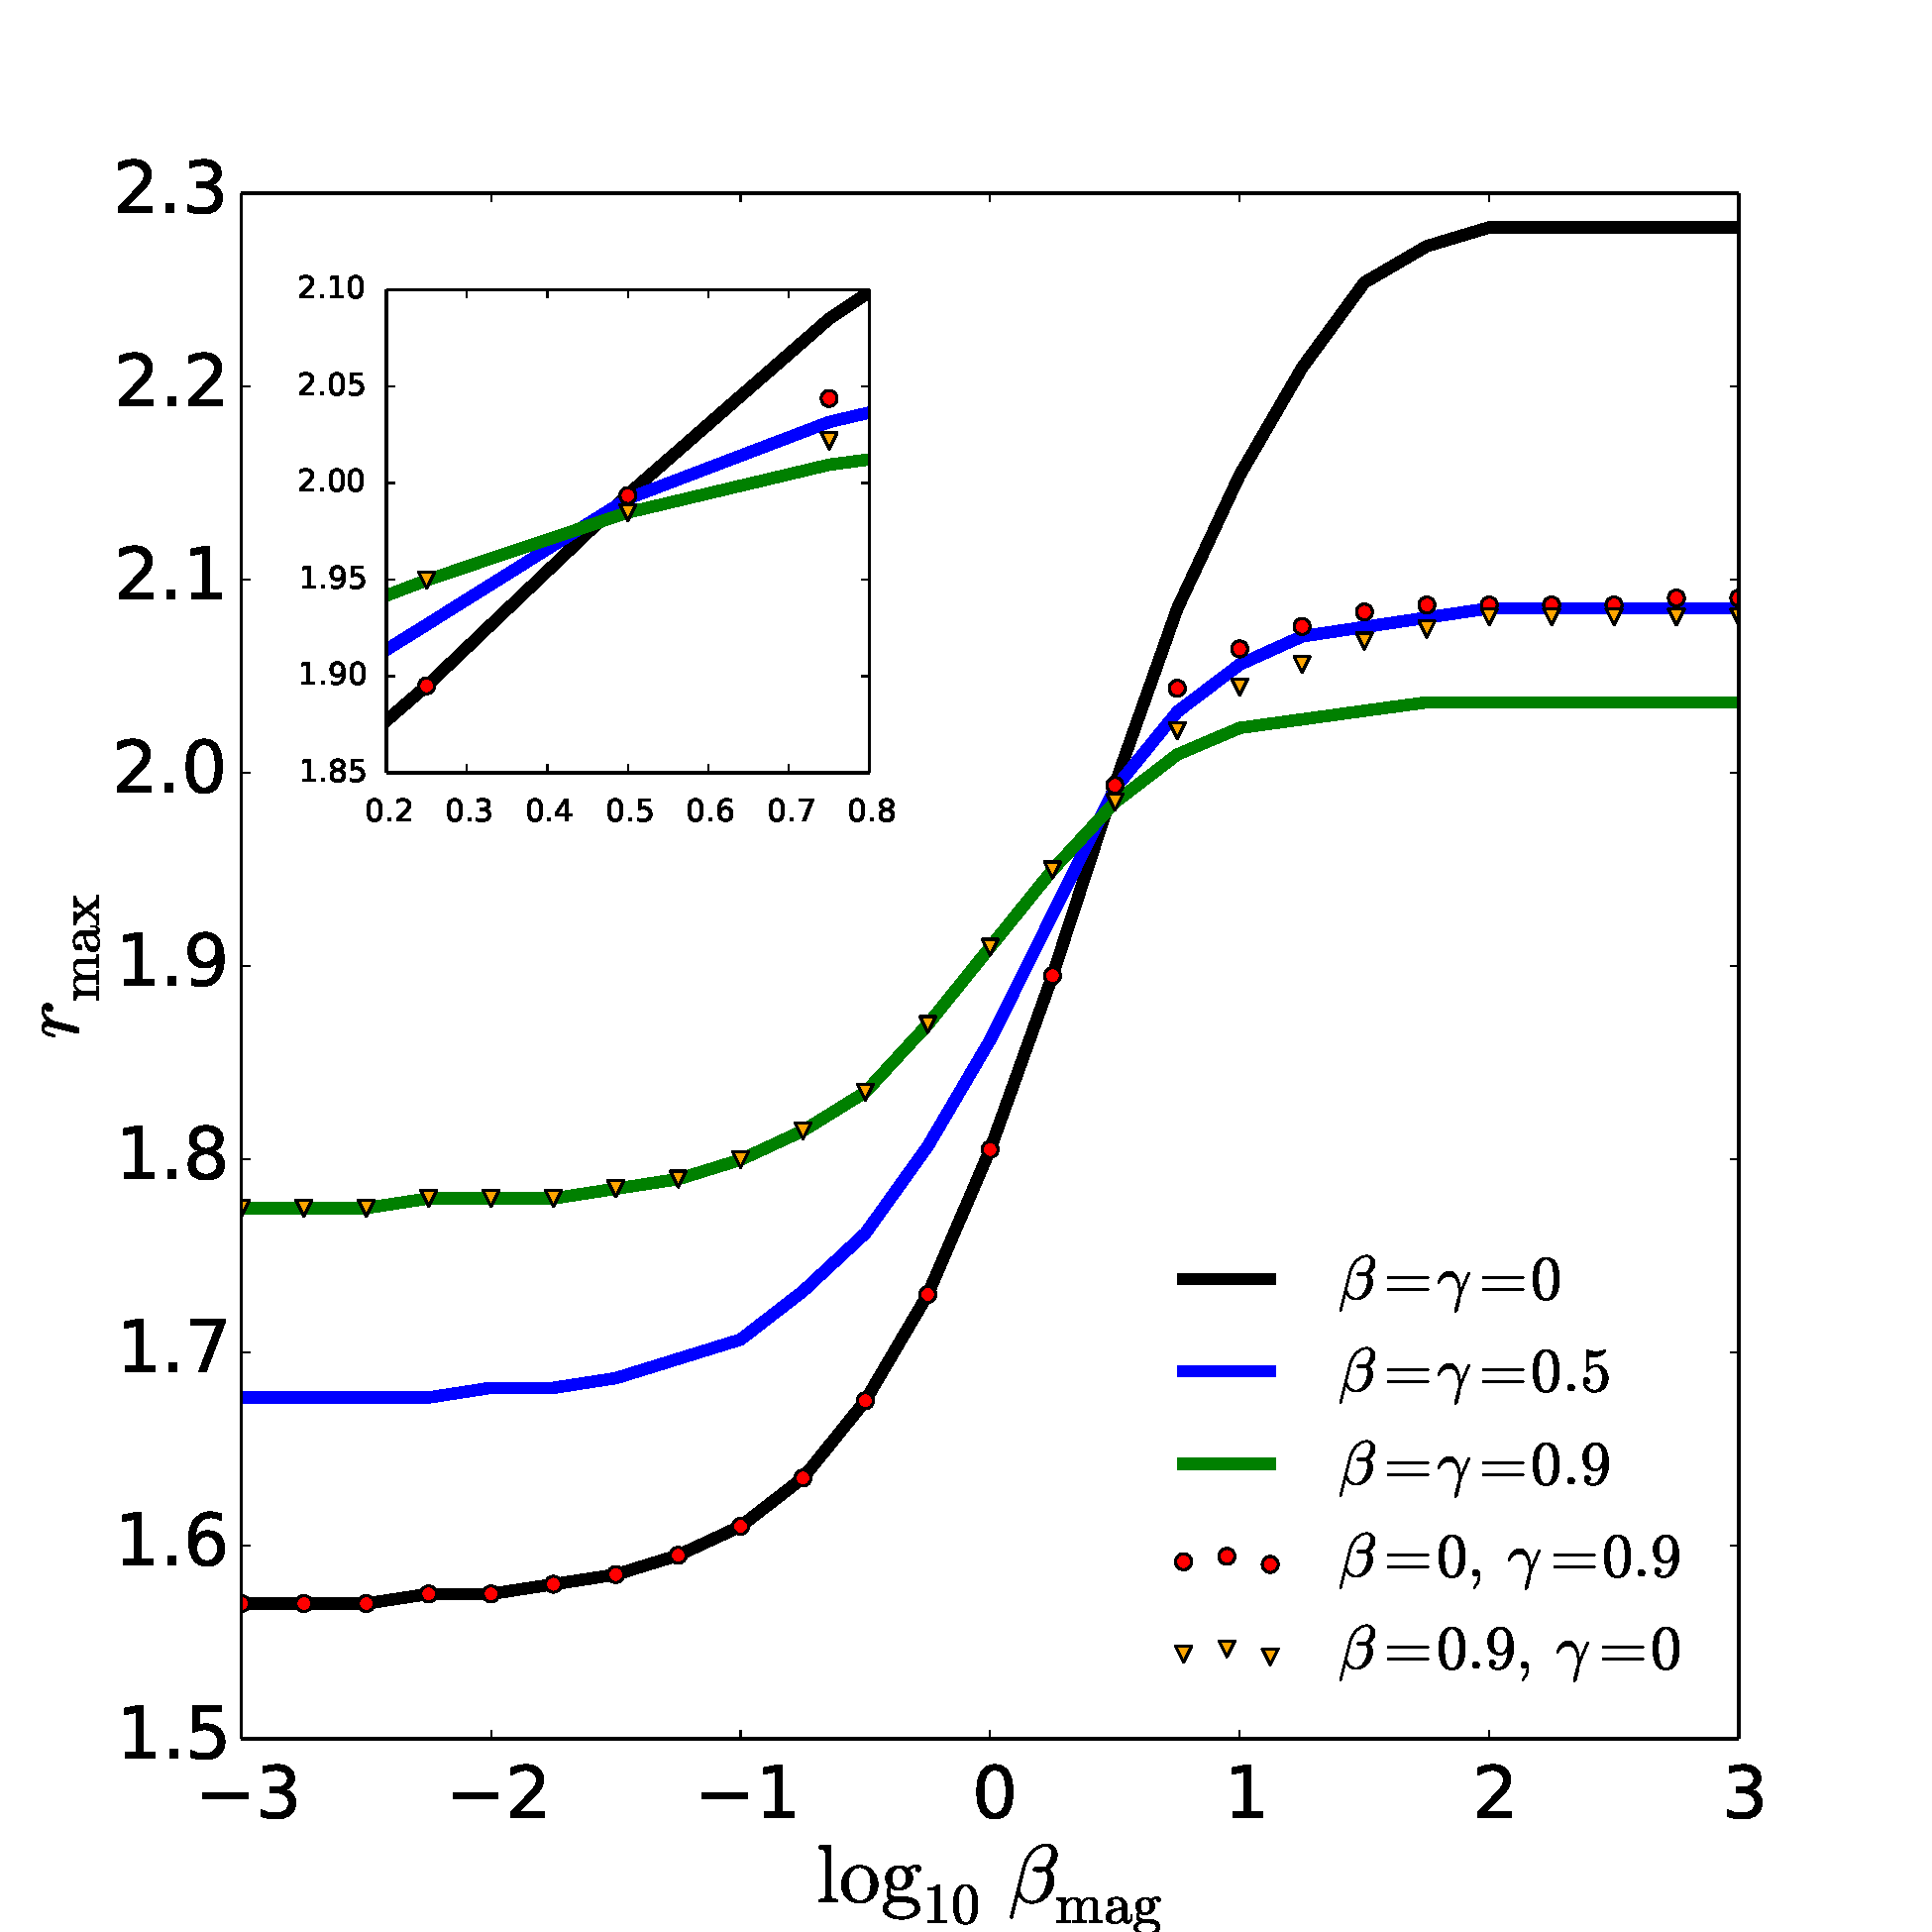
\includegraphics[scale=0.16]{figures/fig6c.pdf}
\caption{The left panel shows the variation of the value for the maximum density with repect to the logarithm of the magnetization parameter. The solid, dashed and dashed lines refer to $a = 0.99$, $0.9$ and $0.5$ respectively and the colour code refers to the models shown in the legend. The middle panel shows the variation of the location of the density maximum (and thermal pressure) with respect to the logarithm of the magnetization parameter for the three models shown in the legend with $a = 0.99$. The right panel shows (also for $a = 0.99$) the variation of the location of the maximum of the magnetic pressure maximum with respect to the logarithm of the magnetization parameter.}
           \label{max-vs-magnetization}%
 \end{figure*}
 
A representative sample of the isodensity surfaces for some of our models appears in Figure~\ref{models}. From left to right the columns of this figure correspond to increasing values of the black hole spin, namely, $a=0.5$, 0.9 and 0.99, while from top to bottom the rows correspond to different combinations of the $\gamma$ and $\beta$ parameters that characterize the ansatz for the angular momentum distribution of~\citet{Qian:2009} (the particular values are indicated in the caption of the figure). The value of the magnetization parameter for all models in this figure is $\beta_{\mathrm{m}_{\mathrm{c}}}
=10^{-3}$. A rapid inspection shows that the structure of the disks noticeable changes when the parameters change. Notice that the spatial scale in all of the plots of this figure has been chosen so as to facilitate the visualization of the disks (which can be fairly small in some cases) and, as such, is different in each plot. A typical Polish doughnut is represented by the model in the top-left panel. As the black hole spin increases, the disks are closer to the black hole and its relative size with respect to the black hole is smaller for all values of $\gamma$ and $\beta$. For $\gamma=0$ the disks are infinite, irrespective of the value of $a$ and $\beta$. As $\gamma$ and $\beta$ increase from 0 to 0.9 (compare the three top rows) the disks become significantly thinner and radially smaller (see also Fig.~\ref{more-profile} below). It is also interesting to note that the maximum value of the density is higher (with respect to the value at the disk center) as the spin increases.

Figure~\ref{magnetization} shows the effects of changing the parameter $\beta_{\mathrm{m}_{\mathrm{c}}}
$ (the magnetization) in the structure of the disks. From left to right the values plotted in each panel are $\beta_{\mathrm{m}_{\mathrm{c}}}
=10^3$, 1, and $10^{-3}$. The model chosen corresponds to $a=0.9$ and $\gamma=\beta=0.5$. The larger the value of $\beta_{\mathrm{m}_{\mathrm{c}}}
$ the less important the effects of the magnetization in the disk structure. Figure~\ref{magnetization} shows that for the kind of magnetic field distribution we are considering, the effects of magnetization are minor. The disk structure remains fairly similar for all values of $\beta_{\mathrm{m}_{\mathrm{c}}}
$ and the only quantitative differences are found in the location of the centre of the disk (which moves inward with decreasing $\beta_{\mathrm{m}_{\mathrm{c}}}
$) and of the range of variation of the isodensity contours (the maximum being slightly larger with decreasing $\beta_{\mathrm{m}_{\mathrm{c}}}
$). This can be more clearly visualized in Figure~\ref{magnetization-profile} which displays the radial profile at the equatorial plane of the density for the same three cases plotted in Fig.~\ref{magnetization}.

Next, we show in Fig.~\ref{more-profile} the corresponding radial profiles at the equatorial plane for the models with black hole spin $a=0.9$. We consider the case $\beta_{\mathrm{m}_{\mathrm{c}}}
=10^{-3}$ (highest magnetization) and the same combination of the $\gamma$ and $\beta$ parameters that we employed in Fig.~\ref{models}. Therefore, this plot depicts the radial profiles of the models occupying the central column of Fig.~\ref{models}. These profiles allow for a clearer quantification of the radial extent of the disks with $\gamma$ and $\beta$. As mentioned in the description of Fig.~\ref{models} as $\gamma$ and $\beta$ increase from 0 to 0.9 (compare black, blue, and green curves) the disks become gradually smaller. At the same time, the radial location of the density maximum increases and the maximum value of the central density (and pressure) decreases. It is worth noticing that the radial profiles of some of the models overlap below a certain radius. More precisely, the black and red curves overlap below $r\sim r_{\mathrm{c}}$ (which corresponds to $\rho \sim 1$) and also the green and orange curves. Also, this figure clearly shows that, besides modifying the thickness of the disk, $\beta$ is the parameter which determines the value of the density (and pressure) maximum. On the other hand, $\gamma$ is only relevant for its radial size.



 
In order to provide a quantitative comparison of the structural differences that appear along the sequence of equilibrium models, we plot in Fig.~\ref{max-vs-magnetization} the variation of the maximum of the density (left panel), the radial location of the maximum of the thermal pressure (middle panel), and the radial location of the maximum of the magnetic pressure (right panel) as a function of the magnetization parameter $\beta_{\mathrm{m}_{\mathrm{c}}}
$. All quantities plotted are measured at the equatorial plane. Let us first consider the left panel. The line type used indicates the value of the black hole spin $a$, namely, a dotted line is for $a=0.5$, a dashed line for $a=0.9$, and a solid line for $a=0.99$. Correspondingly, the colour indicates the value of $\beta$ and $\gamma$ used, namely, red curves correspond to $\gamma=\beta=0$, the blue ones to $\gamma=\beta=0.5$, and the black ones to $\gamma=\beta=0.9$. All curves show the same monotonically decreasing trend with $\beta_{\mathrm{m}_{\mathrm{c}}}
$: for small enough and large enough values of $\beta_{\mathrm{m}_{\mathrm{c}}}
$ the value of the density maximum does not change. However, in the interval $10^{-2}\le \beta_{\mathrm{m}_{\mathrm{c}}}
 \le 10^{2}$, $\rho_{\rm max}$ changes abruptly. The larger the black hole spin the larger the drop in the maximum of the density. For sufficiently large values of $\beta_{\mathrm{m}_{\mathrm{c}}}
$ (small magnetization) the value of $\rho_{\rm max}$ stays constant to the same value irrespective of the black hole rotation.

In the middle panel of Fig.~\ref{max-vs-magnetization} we show the radial location of the maximum of the thermal pressure as a function of $\beta_{\mathrm{m}_{\mathrm{c}}}
$. The black hole spin is $a=0.99$ and the values of $\beta$ and $\gamma$ are indicated in the legend. For all values of $\beta$ and $\gamma$, the maximum of the disk thermal pressure decreases with decreasing $\beta_{\mathrm{m}_{\mathrm{c}}}
$. Below $\beta_{\mathrm{m}_{\mathrm{c}}}
\sim 10^{-3}$ the location of the maximum does not change. The panel also shows that above $\beta_{\mathrm{m}_{\mathrm{c}}}
\sim 10^{3}$ the constant value of $r_{\rm max}$ is the same irrespective of $\beta$ and $\gamma$ as we expected, because for purely hydrodynamic disks, $r_{\mathrm{max}} = r_{\mathrm{c}}$.

The dependence of the location of the maximum of the magnetic pressure with $\beta_{\mathrm{m}_{\mathrm{c}}}
$ is shown in the right panel of Fig.~\ref{max-vs-magnetization}. While the maximum of the magnetic pressure also decreases with decreasing $\beta_{\mathrm{m}_{\mathrm{c}}}
$, the constant value achieved for values above $\beta_{\mathrm{m}_{\mathrm{c}}}
\sim 10^{3}$ does depend on the specific values of $\beta$ and $\gamma$. It must be noted that, for the magnetic pressure, all models seem to cross at roughly the same value of $r_{\rm max}$, as it is more clearly shown in the inset.

It is relevant to add that in the left and middle panels, we do not show the data for the models with $\beta \neq \gamma$ as they coincide with the respective models with the same value of $\beta$. Also, the middle and right panels are only shown for $a=0.99$ because changing the spin parameter of the black hole only yield a change of scale, so if we choose the range of the graph accordingly they are identical irrespective of the value of $a$. 


%%%%%%%%%%%
\section{Conclusions}
\label{conclusions}
%%%%%%%%%%%

In this paper we have presented new sequences of magnetized, non-self-gravitating, equilibrium tori around Kerr black holes by combining two existing approaches~\citep{Komissarov:2006,Qian:2009}. Following~\citet{Qian:2009} the models have been built assuming a form of the angular momentum distribution from which the location and morphology
of surfaces of equal pressure are computed. This ansatz includes as a limiting case the constant angular momentum case originally employed in the construction of thick tori - or Polish doughnuts - and was already used by~\citet{Qian:2009} to build equilibrium sequences of purely hydrodynamical models. Our disks are endowed with a purely toroidal magnetic field, as in the work of~\citet{Komissarov:2006}, which provides the methodology to handle the magnetic terms.

We have discussed the properties of the new models and their dependence on the initial parameters. We have found that the solutions we have built exhibit a saturation-like behaviour for magnetizations over $\beta_{\mathrm{m}_{\mathrm{c}}} \sim 10^{3}$ and below $\beta_{\mathrm{m}_{\mathrm{c}}} \sim 10^{-3}$, so these can be considered as the purely hydrodynamic and MHD limit cases. Also, we have shown the effect of changing of the $\beta$ and $\gamma$ parameters beyond the purely morphological ones in~\citet{Qian:2009}.

In the near future, we plan to extend this work following two paths: i) including the self-gravity of the disks as in the work of~\citet{Stergioulas:2011} and ii) constructing accretions disks around the hairy (both scalar and Proca) black holes described in~\citet{Herdeiro:2014} and~\citet{Herdeiro:2016}.

\begin{acknowledgements}
      Work supported by the Spanish MINECO (grant AYA2015-66899-C2-1-P) and the Generalitat Valenciana (PROMETEOII-2014-069).
\end{acknowledgements}

\bibliographystyle{bibtex/aa}
\bibliography{references}

\end{document}